\documentclass[twoside]{book}

% Packages required by doxygen
\usepackage{fixltx2e}
\usepackage{calc}
\usepackage{doxygen}
\usepackage[export]{adjustbox} % also loads graphicx
\usepackage{graphicx}
\usepackage[utf8]{inputenc}
\usepackage{makeidx}
\usepackage{multicol}
\usepackage{multirow}
\PassOptionsToPackage{warn}{textcomp}
\usepackage{textcomp}
\usepackage[nointegrals]{wasysym}
\usepackage[table]{xcolor}

% NLS support packages
\usepackage[french]{babel}

% Font selection
\usepackage[T1]{fontenc}
\usepackage[scaled=.90]{helvet}
\usepackage{courier}
\usepackage{amssymb}
\usepackage{sectsty}
\renewcommand{\familydefault}{\sfdefault}
\allsectionsfont{%
  \fontseries{bc}\selectfont%
  \color{darkgray}%
}
\renewcommand{\DoxyLabelFont}{%
  \fontseries{bc}\selectfont%
  \color{darkgray}%
}
\newcommand{\+}{\discretionary{\mbox{\scriptsize$\hookleftarrow$}}{}{}}

% Page & text layout
\usepackage{geometry}
\geometry{%
  a4paper,%
  top=2.5cm,%
  bottom=2.5cm,%
  left=2.5cm,%
  right=2.5cm%
}
\tolerance=750
\hfuzz=15pt
\hbadness=750
\setlength{\emergencystretch}{15pt}
\setlength{\parindent}{0cm}
\setlength{\parskip}{3ex plus 2ex minus 2ex}
\makeatletter
\renewcommand{\paragraph}{%
  \@startsection{paragraph}{4}{0ex}{-1.0ex}{1.0ex}{%
    \normalfont\normalsize\bfseries\SS@parafont%
  }%
}
\renewcommand{\subparagraph}{%
  \@startsection{subparagraph}{5}{0ex}{-1.0ex}{1.0ex}{%
    \normalfont\normalsize\bfseries\SS@subparafont%
  }%
}
\makeatother

% Headers & footers
\usepackage{fancyhdr}
\pagestyle{fancyplain}
\fancyhead[LE]{\fancyplain{}{\bfseries\thepage}}
\fancyhead[CE]{\fancyplain{}{}}
\fancyhead[RE]{\fancyplain{}{\bfseries\leftmark}}
\fancyhead[LO]{\fancyplain{}{\bfseries\rightmark}}
\fancyhead[CO]{\fancyplain{}{}}
\fancyhead[RO]{\fancyplain{}{\bfseries\thepage}}
\fancyfoot[LE]{\fancyplain{}{}}
\fancyfoot[CE]{\fancyplain{}{}}
\fancyfoot[RE]{\fancyplain{}{\bfseries\scriptsize Généré par Doxygen }}
\fancyfoot[LO]{\fancyplain{}{\bfseries\scriptsize Généré par Doxygen }}
\fancyfoot[CO]{\fancyplain{}{}}
\fancyfoot[RO]{\fancyplain{}{}}
\renewcommand{\footrulewidth}{0.4pt}
\renewcommand{\chaptermark}[1]{%
  \markboth{#1}{}%
}
\renewcommand{\sectionmark}[1]{%
  \markright{\thesection\ #1}%
}

% Indices & bibliography
\usepackage{natbib}
\usepackage[titles]{tocloft}
\setcounter{tocdepth}{3}
\setcounter{secnumdepth}{5}
\makeindex

% Hyperlinks (required, but should be loaded last)
\usepackage{ifpdf}
\ifpdf
  \usepackage[pdftex,pagebackref=true]{hyperref}
\else
  \usepackage[ps2pdf,pagebackref=true]{hyperref}
\fi
\hypersetup{%
  colorlinks=true,%
  linkcolor=blue,%
  citecolor=blue,%
  unicode%
}

% Custom commands
\newcommand{\clearemptydoublepage}{%
  \newpage{\pagestyle{empty}\cleardoublepage}%
}

\usepackage{caption}
\captionsetup{labelsep=space,justification=centering,font={bf},singlelinecheck=off,skip=4pt,position=top}

%===== C O N T E N T S =====

\begin{document}

% Titlepage & ToC
\hypersetup{pageanchor=false,
             bookmarksnumbered=true,
             pdfencoding=unicode
            }
\pagenumbering{alph}
\begin{titlepage}
\vspace*{7cm}
\begin{center}%
{\Large Poke\+Peip \\[1ex]\large Beta 1.\+0 }\\
\vspace*{1cm}
{\large Généré par Doxygen 1.8.13}\\
\end{center}
\end{titlepage}
\clearemptydoublepage
\pagenumbering{roman}
\tableofcontents
\clearemptydoublepage
\pagenumbering{arabic}
\hypersetup{pageanchor=true}

%--- Begin generated contents ---
\chapter{Index hiérarchique}
\section{Class Hierarchy}
This inheritance list is sorted roughly, but not completely, alphabetically\+:\begin{DoxyCompactList}
\item \contentsline{section}{Aff\+S\+F\+ML}{\pageref{class_aff_s_f_m_l}}{}
\begin{DoxyCompactList}
\item \contentsline{section}{S\+F\+M\+L\+Combat\+IA}{\pageref{class_s_f_m_l_combat_i_a}}{}
\end{DoxyCompactList}
\item \contentsline{section}{Animation}{\pageref{class_animation}}{}
\item \contentsline{section}{Attaque}{\pageref{class_attaque}}{}
\item \contentsline{section}{Combat}{\pageref{class_combat}}{}
\item Drawable\begin{DoxyCompactList}
\item \contentsline{section}{Animated\+Sprite}{\pageref{class_animated_sprite}}{}
\end{DoxyCompactList}
\item \contentsline{section}{Objet}{\pageref{class_objet}}{}
\item \contentsline{section}{Personnage}{\pageref{class_personnage}}{}
\begin{DoxyCompactList}
\item \contentsline{section}{Adversaire}{\pageref{class_adversaire}}{}
\item \contentsline{section}{Joueur}{\pageref{class_joueur}}{}
\end{DoxyCompactList}
\item \contentsline{section}{Pokedex}{\pageref{struct_pokedex}}{}
\item \contentsline{section}{Pokemon}{\pageref{class_pokemon}}{}
\item \contentsline{section}{Sac}{\pageref{class_sac}}{}
\item \contentsline{section}{S\+F\+M\+L\+Charger}{\pageref{class_s_f_m_l_charger}}{}
\item \contentsline{section}{S\+F\+M\+L\+Menu}{\pageref{class_s_f_m_l_menu}}{}
\item \contentsline{section}{S\+F\+M\+L\+Pokedex}{\pageref{class_s_f_m_l_pokedex}}{}
\item Transformable\begin{DoxyCompactList}
\item \contentsline{section}{Animated\+Sprite}{\pageref{class_animated_sprite}}{}
\end{DoxyCompactList}
\end{DoxyCompactList}

\chapter{Index des classes}
\section{Liste des classes}
Liste des classes, structures, unions et interfaces avec une brève description \+:\begin{DoxyCompactList}
\item\contentsline{section}{\hyperlink{class_adversaire}{Adversaire} \\*Classe \hyperlink{class_adversaire}{Adversaire} hérité de la classe \hyperlink{class_personnage}{Personnage} qui gère un adversaire et qui contient son nombre de défaites,de victoires,son niveau et son argent }{\pageref{class_adversaire}}{}
\item\contentsline{section}{\hyperlink{class_attaque}{Attaque} \\*La classe représentant les Attaques des \hyperlink{class_pokemon}{Pokemon} }{\pageref{class_attaque}}{}
\item\contentsline{section}{\hyperlink{class_combat}{Combat} \\*La classe gérant le combat }{\pageref{class_combat}}{}
\item\contentsline{section}{\hyperlink{class_joueur}{Joueur} \\*Classe \hyperlink{class_joueur}{Joueur} hérité de la classe \hyperlink{class_personnage}{Personnage} qui gère un joueur et qui contient son nombre de défaites,de victoires,son niveau et son argent }{\pageref{class_joueur}}{}
\item\contentsline{section}{\hyperlink{class_objet}{Objet} \\*Classe \hyperlink{class_objet}{Objet} qui gère un objet et qui contient son type d\textquotesingle{}objet,son nom,sa description et sa quantité }{\pageref{class_objet}}{}
\item\contentsline{section}{\hyperlink{class_personnage}{Personnage} \\*Classe \hyperlink{class_personnage}{Personnage} qui gère un personnage et qui contient son nom, son équipe pokémon et son sac }{\pageref{class_personnage}}{}
\item\contentsline{section}{\hyperlink{class_pokemon}{Pokemon} }{\pageref{class_pokemon}}{}
\item\contentsline{section}{\hyperlink{class_sac}{Sac} }{\pageref{class_sac}}{}
\item\contentsline{section}{\hyperlink{class_s_f_m_l_charger}{S\+F\+M\+L\+Charger} \\*Classe \hyperlink{class_s_f_m_l_charger}{S\+F\+M\+L\+Charger} qui gère l\textquotesingle{}affichage du chargement des joueurs }{\pageref{class_s_f_m_l_charger}}{}
\item\contentsline{section}{\hyperlink{class_s_f_m_l_combat}{S\+F\+M\+L\+Combat} \\*La classe gérant la partie I\+HM du combat }{\pageref{class_s_f_m_l_combat}}{}
\item\contentsline{section}{\hyperlink{class_s_f_m_l_menu}{S\+F\+M\+L\+Menu} \\*La classe gérant le principale affichage graphique }{\pageref{class_s_f_m_l_menu}}{}
\item\contentsline{section}{\hyperlink{class_s_f_m_l_pokedex}{S\+F\+M\+L\+Pokedex} \\*La classe gérant le principale affichage graphique }{\pageref{class_s_f_m_l_pokedex}}{}
\end{DoxyCompactList}

\chapter{Index des fichiers}
\section{Liste des fichiers}
Liste de tous les fichiers documentés avec une brève description \+:\begin{DoxyCompactList}
\item\contentsline{section}{/home/corentin/\+Documents/lifap4/src/\+Attaque/\hyperlink{_attaque_8cpp}{Attaque.\+cpp} \\*Fichier d\textquotesingle{}implémentation de la classe \hyperlink{_attaque_8cpp}{Attaque.\+cpp} }{\pageref{_attaque_8cpp}}{}
\item\contentsline{section}{/home/corentin/\+Documents/lifap4/src/\+Attaque/\hyperlink{_attaque_8h}{Attaque.\+h} \\*Documentation du module \hyperlink{class_attaque}{Attaque}. Le module \hyperlink{class_attaque}{Attaque} représente les attaques qui seront utilisés par les \hyperlink{class_pokemon}{Pokemon} durant leur combat }{\pageref{_attaque_8h}}{}
\item\contentsline{section}{/home/corentin/\+Documents/lifap4/src/\+Combat/\hyperlink{_combat_8cpp}{Combat.\+cpp} \\*Fichier d\textquotesingle{}implémentation de la classe \hyperlink{_combat_8cpp}{Combat.\+cpp} }{\pageref{_combat_8cpp}}{}
\item\contentsline{section}{/home/corentin/\+Documents/lifap4/src/\+Combat/\hyperlink{_combat_8h}{Combat.\+h} \\*Documentation du module \hyperlink{class_combat}{Combat}. Le module \hyperlink{class_combat}{Combat} représente un combat entre deux joueurs, et chaque joueur combat avec une équipe de 6 \hyperlink{class_pokemon}{Pokemon} }{\pageref{_combat_8h}}{}
\item\contentsline{section}{/home/corentin/\+Documents/lifap4/src/\+Objet/\hyperlink{_objet_8cpp}{Objet.\+cpp} \\*Fichier d\textquotesingle{}implémentation de la classe \hyperlink{class_objet}{Objet} }{\pageref{_objet_8cpp}}{}
\item\contentsline{section}{/home/corentin/\+Documents/lifap4/src/\+Objet/\hyperlink{_objet_8h}{Objet.\+h} \\*Module gérant un objet dans le jeu Poke\+P\+E\+IP }{\pageref{_objet_8h}}{}
\item\contentsline{section}{/home/corentin/\+Documents/lifap4/src/\+Personnage/\hyperlink{_personnage_8cpp}{Personnage.\+cpp} \\*Fichier d\textquotesingle{}implémentation de la classe \hyperlink{class_personnage}{Personnage} }{\pageref{_personnage_8cpp}}{}
\item\contentsline{section}{/home/corentin/\+Documents/lifap4/src/\+Personnage/\hyperlink{_personnage_8h}{Personnage.\+h} \\*Module gérant un \hyperlink{class_personnage}{Personnage} dans Poke\+P\+E\+IP }{\pageref{_personnage_8h}}{}
\item\contentsline{section}{/home/corentin/\+Documents/lifap4/src/\+Pokemon/\hyperlink{_pokemon_8cpp}{Pokemon.\+cpp} \\*Fichier d\textquotesingle{}implémentation de la classe \hyperlink{class_pokemon}{Pokemon} }{\pageref{_pokemon_8cpp}}{}
\item\contentsline{section}{/home/corentin/\+Documents/lifap4/src/\+Pokemon/\hyperlink{_pokemon_8h}{Pokemon.\+h} \\*Classe \hyperlink{class_pokemon}{Pokemon} qui gère un pokémon et qui contient son type d\textquotesingle{}objet,son nom,sa description et sa quantité }{\pageref{_pokemon_8h}}{}
\item\contentsline{section}{/home/corentin/\+Documents/lifap4/src/\+Sac/\hyperlink{_sac_8cpp}{Sac.\+cpp} \\*Fichier d\textquotesingle{}implémentation de la classe \hyperlink{class_sac}{Sac} }{\pageref{_sac_8cpp}}{}
\item\contentsline{section}{/home/corentin/\+Documents/lifap4/src/\+Sac/{\bfseries Sac.\+h} }{\pageref{_sac_8h}}{}
\item\contentsline{section}{/home/corentin/\+Documents/lifap4/src/\+S\+F\+M\+L\+Charger/\hyperlink{_s_f_m_l_charger_8cpp}{S\+F\+M\+L\+Charger.\+cpp} \\*Fichier d\textquotesingle{}implémentation de la classe \hyperlink{_s_f_m_l_charger_8cpp}{S\+F\+M\+L\+Charger.\+cpp} }{\pageref{_s_f_m_l_charger_8cpp}}{}
\item\contentsline{section}{/home/corentin/\+Documents/lifap4/src/\+S\+F\+M\+L\+Charger/{\bfseries S\+F\+M\+L\+Charger.\+h} }{\pageref{_s_f_m_l_charger_8h}}{}
\item\contentsline{section}{/home/corentin/\+Documents/lifap4/src/\+S\+F\+M\+L\+Combat/\hyperlink{_s_f_m_l_8cpp}{S\+F\+M\+L.\+cpp} \\*Fichier d\textquotesingle{}implémentation de la classe \hyperlink{_s_f_m_l_8cpp}{S\+F\+M\+L.\+cpp} }{\pageref{_s_f_m_l_8cpp}}{}
\item\contentsline{section}{/home/corentin/\+Documents/lifap4/src/\+S\+F\+M\+L\+Combat/\hyperlink{_s_f_m_l_8h}{S\+F\+M\+L.\+h} \\*Documentation du module \hyperlink{_s_f_m_l_8cpp}{S\+F\+M\+L.\+cpp} }{\pageref{_s_f_m_l_8h}}{}
\item\contentsline{section}{/home/corentin/\+Documents/lifap4/src/\+S\+F\+M\+L\+Menu/\hyperlink{_s_f_m_l_menu_8cpp}{S\+F\+M\+L\+Menu.\+cpp} \\*Fichier d\textquotesingle{}implémentation de la classe \hyperlink{_s_f_m_l_menu_8cpp}{S\+F\+M\+L\+Menu.\+cpp} }{\pageref{_s_f_m_l_menu_8cpp}}{}
\item\contentsline{section}{/home/corentin/\+Documents/lifap4/src/\+S\+F\+M\+L\+Menu/\hyperlink{_s_f_m_l_menu_8h}{S\+F\+M\+L\+Menu.\+h} \\*Documentation du module \hyperlink{class_s_f_m_l_menu}{S\+F\+M\+L\+Menu} }{\pageref{_s_f_m_l_menu_8h}}{}
\item\contentsline{section}{/home/corentin/\+Documents/lifap4/src/\+S\+F\+M\+L\+Pokedex/\hyperlink{_s_f_m_l_pokedex_8cpp}{S\+F\+M\+L\+Pokedex.\+cpp} \\*Fichier d\textquotesingle{}implémentation de la classe \hyperlink{_s_f_m_l_pokedex_8cpp}{S\+F\+M\+L\+Pokedex.\+cpp} }{\pageref{_s_f_m_l_pokedex_8cpp}}{}
\item\contentsline{section}{/home/corentin/\+Documents/lifap4/src/\+S\+F\+M\+L\+Pokedex/\hyperlink{_s_f_m_l_pokedex_8h}{S\+F\+M\+L\+Pokedex.\+h} \\*Documentation du module \hyperlink{class_s_f_m_l_pokedex}{S\+F\+M\+L\+Pokedex} }{\pageref{_s_f_m_l_pokedex_8h}}{}
\end{DoxyCompactList}

\chapter{Documentation des classes}
\hypertarget{class_adversaire}{}\section{Adversaire Class Reference}
\label{class_adversaire}\index{Adversaire@{Adversaire}}


Inheritance diagram for Adversaire\+:
\nopagebreak
\begin{figure}[H]
\begin{center}
\leavevmode
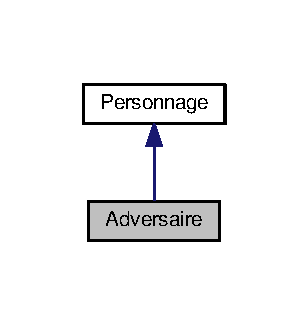
\includegraphics[width=148pt]{class_adversaire__inherit__graph}
\end{center}
\end{figure}


Collaboration diagram for Adversaire\+:
\nopagebreak
\begin{figure}[H]
\begin{center}
\leavevmode
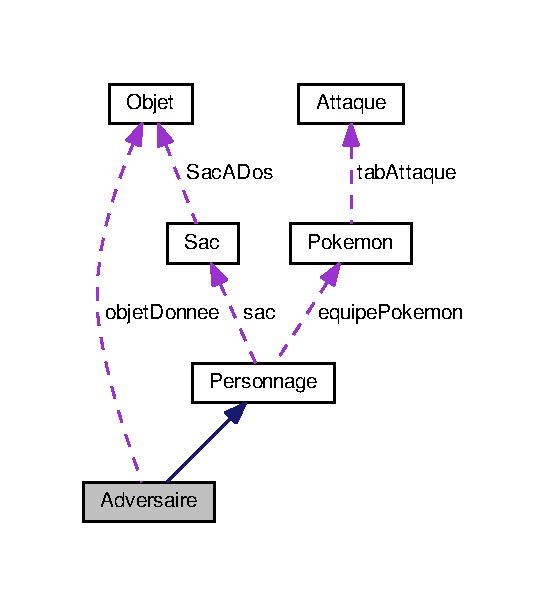
\includegraphics[width=148pt]{class_adversaire__coll__graph}
\end{center}
\end{figure}
\subsection*{Public Member Functions}
\begin{DoxyCompactItemize}
\item 
\mbox{\Hypertarget{class_adversaire_acc1711c4359e7d5be90f46f247bc773c}\label{class_adversaire_acc1711c4359e7d5be90f46f247bc773c}} 
{\bfseries Adversaire} (const std\+::string \&n, const std\+::string \&d, char s)
\item 
\mbox{\Hypertarget{class_adversaire_a8b95db33d9233f0edcc2d870cc2242c3}\label{class_adversaire_a8b95db33d9233f0edcc2d870cc2242c3}} 
unsigned int {\bfseries get\+Argent\+Donnee} () const
\item 
\mbox{\Hypertarget{class_adversaire_a9938730269f971643fcd039efcfa0010}\label{class_adversaire_a9938730269f971643fcd039efcfa0010}} 
\hyperlink{class_objet}{Objet} {\bfseries get\+Objet\+Donne} () const
\item 
\mbox{\Hypertarget{class_adversaire_ab8371ffdc0fc9a934212e05fbf3fedc2}\label{class_adversaire_ab8371ffdc0fc9a934212e05fbf3fedc2}} 
void {\bfseries set\+Argent\+Donnee} (unsigned int i)
\item 
\mbox{\Hypertarget{class_adversaire_a96bed950b5172bbda0a2ddab2b1ff68c}\label{class_adversaire_a96bed950b5172bbda0a2ddab2b1ff68c}} 
void {\bfseries set\+Objet\+Donne} (const \hyperlink{class_objet}{Objet} \&o)
\item 
\mbox{\Hypertarget{class_adversaire_ac0a12a8a849f87161ccc844cee731374}\label{class_adversaire_ac0a12a8a849f87161ccc844cee731374}} 
void {\bfseries detruire\+Objet} ()
\item 
\mbox{\Hypertarget{class_adversaire_a5540f25c07c308dcc31328501a980c1c}\label{class_adversaire_a5540f25c07c308dcc31328501a980c1c}} 
void {\bfseries charger\+Adversaire} (unsigned int niveau)
\end{DoxyCompactItemize}


The documentation for this class was generated from the following files\+:\begin{DoxyCompactItemize}
\item 
/home/corentin/\+Documents/lifap4/src/\+Personnage/Personnage.\+h\item 
/home/corentin/\+Documents/lifap4/src/\+Personnage/Personnage.\+cpp\end{DoxyCompactItemize}

\hypertarget{class_attaque}{}\section{Attaque Class Reference}
\label{class_attaque}\index{Attaque@{Attaque}}
\subsection*{Public Member Functions}
\begin{DoxyCompactItemize}
\item 
\mbox{\Hypertarget{class_attaque_a0d06199581234d41d63a842b3efa3716}\label{class_attaque_a0d06199581234d41d63a842b3efa3716}} 
{\bfseries Attaque} (const std\+::string \&nom\+Attaque, const Type \&t, unsigned int pp, unsigned int Puissance, unsigned int Precision, const Effet\+Attaque \&eA, std \+::string desc, const Type\+Attaque \&tA)
\item 
\mbox{\Hypertarget{class_attaque_a6e0b308dd1d9ddab688378e2630cb597}\label{class_attaque_a6e0b308dd1d9ddab688378e2630cb597}} 
void {\bfseries set\+Nb\+PP} (unsigned int nb)
\item 
\mbox{\Hypertarget{class_attaque_a15bcb3d5d9add6357427cfb399e5584a}\label{class_attaque_a15bcb3d5d9add6357427cfb399e5584a}} 
void {\bfseries set\+Nom} (std\+::string nom)
\item 
\mbox{\Hypertarget{class_attaque_a92ae062d505e82c80621069dc6a917d1}\label{class_attaque_a92ae062d505e82c80621069dc6a917d1}} 
unsigned int {\bfseries get\+Puissance} () const
\item 
\mbox{\Hypertarget{class_attaque_ada8c22f0becc001b46e6a7f2da00a1ef}\label{class_attaque_ada8c22f0becc001b46e6a7f2da00a1ef}} 
unsigned int {\bfseries get\+Precision} () const
\item 
\mbox{\Hypertarget{class_attaque_aa2e4cf0577df21c32295b757bc6e0dc5}\label{class_attaque_aa2e4cf0577df21c32295b757bc6e0dc5}} 
std \+::string {\bfseries get\+Description} () const
\item 
\mbox{\Hypertarget{class_attaque_a1776bbc505173b30dc6577a806228a78}\label{class_attaque_a1776bbc505173b30dc6577a806228a78}} 
Effet\+Attaque {\bfseries get\+Effet} () const
\item 
\mbox{\Hypertarget{class_attaque_aa95b1e494a9c24dfd28c585e46cd1eb8}\label{class_attaque_aa95b1e494a9c24dfd28c585e46cd1eb8}} 
unsigned int {\bfseries get\+Nb\+PP} () const
\item 
\mbox{\Hypertarget{class_attaque_a651deeca5e47dd04929bd1c9d013c86e}\label{class_attaque_a651deeca5e47dd04929bd1c9d013c86e}} 
unsigned int {\bfseries get\+Nb\+P\+P\+Max} () const
\item 
\mbox{\Hypertarget{class_attaque_acb25c596d5b90b2330d3188749bc130d}\label{class_attaque_acb25c596d5b90b2330d3188749bc130d}} 
Type\+Attaque {\bfseries get\+Type\+Attaque} () const
\item 
\mbox{\Hypertarget{class_attaque_a2d3e865f856f681f79934680b25ac372}\label{class_attaque_a2d3e865f856f681f79934680b25ac372}} 
std \+::string {\bfseries get\+Nom} () const
\item 
\mbox{\Hypertarget{class_attaque_af43d72ec9abad98f04e21e245cece692}\label{class_attaque_af43d72ec9abad98f04e21e245cece692}} 
Type {\bfseries get\+Type} () const
\item 
\mbox{\Hypertarget{class_attaque_ab1ddce65c74895578f145763b7ae98ef}\label{class_attaque_ab1ddce65c74895578f145763b7ae98ef}} 
void {\bfseries rentrer\+Attaque\+Fichier} (const std \+::string \&fichier)
\item 
\mbox{\Hypertarget{class_attaque_a8017dbfbf4af62e113d27d093a2786c6}\label{class_attaque_a8017dbfbf4af62e113d27d093a2786c6}} 
void {\bfseries test\+Regression} ()
\item 
\mbox{\Hypertarget{class_attaque_ad6320c58f467865c778aae13c75c558f}\label{class_attaque_ad6320c58f467865c778aae13c75c558f}} 
void {\bfseries baisser\+Nb\+PP} ()
\item 
\mbox{\Hypertarget{class_attaque_a21b14fe41db692f8e38aa1821a3519b9}\label{class_attaque_a21b14fe41db692f8e38aa1821a3519b9}} 
\hyperlink{class_attaque}{Attaque} \& {\bfseries operator=} (const \hyperlink{class_attaque}{Attaque} \&attaque)
\end{DoxyCompactItemize}


The documentation for this class was generated from the following files\+:\begin{DoxyCompactItemize}
\item 
/home/corentin/\+Documents/lifap4/src/\+Attaque/Attaque.\+h\item 
/home/corentin/\+Documents/lifap4/src/\+Attaque/Attaque.\+cpp\end{DoxyCompactItemize}

\hypertarget{class_combat}{}\section{Combat Class Reference}
\label{class_combat}\index{Combat@{Combat}}
\subsection*{Public Member Functions}
\begin{DoxyCompactItemize}
\item 
\mbox{\Hypertarget{class_combat_af420be03c806ef847c0542ab0d7223f9}\label{class_combat_af420be03c806ef847c0542ab0d7223f9}} 
{\bfseries Combat} (\hyperlink{class_joueur}{Joueur} \&perso, \hyperlink{class_adversaire}{Adversaire} \&dress)
\item 
\mbox{\Hypertarget{class_combat_a6f3c9e5df27cfb30359dcb0425a45f6d}\label{class_combat_a6f3c9e5df27cfb30359dcb0425a45f6d}} 
\hyperlink{class_pokemon}{Pokemon} {\bfseries get\+Poke\+Perso} () const
\item 
\mbox{\Hypertarget{class_combat_aa06e658e7fb4ab91174ba4d832588bae}\label{class_combat_aa06e658e7fb4ab91174ba4d832588bae}} 
\hyperlink{class_pokemon}{Pokemon} {\bfseries get\+Poke\+Adversaire} () const
\item 
\mbox{\Hypertarget{class_combat_a9a44a83a9c1fe5d67f0b620dab547e56}\label{class_combat_a9a44a83a9c1fe5d67f0b620dab547e56}} 
\hyperlink{class_pokemon}{Pokemon} $\ast$ {\bfseries get\+Poke\+Perso\+Ref} ()
\item 
\mbox{\Hypertarget{class_combat_a4f02e335d825eb98b64d5410a590b9f8}\label{class_combat_a4f02e335d825eb98b64d5410a590b9f8}} 
\hyperlink{class_pokemon}{Pokemon} $\ast$ {\bfseries get\+Poke\+Adversaire\+Ref} ()
\item 
\mbox{\Hypertarget{class_combat_a3784ddbca993b5ad0fb0d4dd382f919a}\label{class_combat_a3784ddbca993b5ad0fb0d4dd382f919a}} 
\hyperlink{class_joueur}{Joueur} {\bfseries get\+Joueur} () const
\item 
\mbox{\Hypertarget{class_combat_a018644148fc62da9c8abfafc166713c4}\label{class_combat_a018644148fc62da9c8abfafc166713c4}} 
\hyperlink{class_adversaire}{Adversaire} {\bfseries get\+Adversaire} () const
\item 
\mbox{\Hypertarget{class_combat_af72bd31264a8cdeeb3f3f8c30c727d33}\label{class_combat_af72bd31264a8cdeeb3f3f8c30c727d33}} 
\hyperlink{class_joueur}{Joueur} $\ast$ {\bfseries get\+Joueur\+Ref} ()
\item 
\mbox{\Hypertarget{class_combat_a59088f5725884e9c363ad72a946c82ef}\label{class_combat_a59088f5725884e9c363ad72a946c82ef}} 
\hyperlink{class_adversaire}{Adversaire} $\ast$ {\bfseries get\+Adversaire\+Ref} ()
\item 
\mbox{\Hypertarget{class_combat_ac02efb89c200ba49e86bb74fdc7dba21}\label{class_combat_ac02efb89c200ba49e86bb74fdc7dba21}} 
int {\bfseries get\+Joueur\+Gagnant} ()
\item 
\mbox{\Hypertarget{class_combat_aed2119127fb9b7ed023dd481927c27aa}\label{class_combat_aed2119127fb9b7ed023dd481927c27aa}} 
int {\bfseries get\+Qui\+Joue} () const
\item 
\mbox{\Hypertarget{class_combat_a292caf86cb2c8ecbf9ecd055e6a028c0}\label{class_combat_a292caf86cb2c8ecbf9ecd055e6a028c0}} 
void {\bfseries set\+Qui\+Joue} (unsigned int i)
\item 
\mbox{\Hypertarget{class_combat_a7ff4ea33e3bafa37fd8f5a0754955b4f}\label{class_combat_a7ff4ea33e3bafa37fd8f5a0754955b4f}} 
void {\bfseries set\+J1} (\hyperlink{class_joueur}{Joueur} \&joueur)
\item 
\mbox{\Hypertarget{class_combat_a2093b3be4975b62aa546d54f108834f3}\label{class_combat_a2093b3be4975b62aa546d54f108834f3}} 
void {\bfseries set\+J2} (\hyperlink{class_adversaire}{Adversaire} \&adversaire)
\item 
\mbox{\Hypertarget{class_combat_a567eab49812ecbd2d694e8cf064e800a}\label{class_combat_a567eab49812ecbd2d694e8cf064e800a}} 
void {\bfseries changer\+De\+Pokemon} (unsigned int i)
\item 
\mbox{\Hypertarget{class_combat_a2848c91d76a09943dd5effb1904f1937}\label{class_combat_a2848c91d76a09943dd5effb1904f1937}} 
void {\bfseries changer\+Qui\+Joue} ()
\item 
\mbox{\Hypertarget{class_combat_a735c71f16ce62c1dbe3a40cdca6ca44b}\label{class_combat_a735c71f16ce62c1dbe3a40cdca6ca44b}} 
bool {\bfseries lancer\+Attaque} (unsigned int i)
\item 
\mbox{\Hypertarget{class_combat_a3ab678df151ed9210806f89d1aeb47ab}\label{class_combat_a3ab678df151ed9210806f89d1aeb47ab}} 
bool {\bfseries utiliser\+Objet} (\hyperlink{class_pokemon}{Pokemon} \&Pkmn, unsigned int i)
\item 
\mbox{\Hypertarget{class_combat_abbaadce2f31d9b12645481cc74a021b2}\label{class_combat_abbaadce2f31d9b12645481cc74a021b2}} 
bool {\bfseries fin\+De\+Jeu} ()
\item 
\mbox{\Hypertarget{class_combat_ad1fb106750152c5008a04efc5b2b432d}\label{class_combat_ad1fb106750152c5008a04efc5b2b432d}} 
int {\bfseries calcul\+Priorite} ()
\item 
\mbox{\Hypertarget{class_combat_ab8ad53e804e2dccddf100af63d5892e6}\label{class_combat_ab8ad53e804e2dccddf100af63d5892e6}} 
void {\bfseries test\+Regression} ()
\end{DoxyCompactItemize}


The documentation for this class was generated from the following files\+:\begin{DoxyCompactItemize}
\item 
/home/corentin/\+Documents/lifap4/src/\+Combat/Combat.\+h\item 
/home/corentin/\+Documents/lifap4/src/\+Combat/Combat.\+cpp\end{DoxyCompactItemize}

\hypertarget{class_joueur}{}\section{Référence de la classe Joueur}
\label{class_joueur}\index{Joueur@{Joueur}}


Classe \hyperlink{class_joueur}{Joueur} hérité de la classe \hyperlink{class_personnage}{Personnage} qui gère un joueur et qui contient son nombre de défaites,de victoires,son niveau et son argent.  




{\ttfamily \#include $<$Personnage.\+h$>$}



Graphe d\textquotesingle{}héritage de Joueur\+:\nopagebreak
\begin{figure}[H]
\begin{center}
\leavevmode
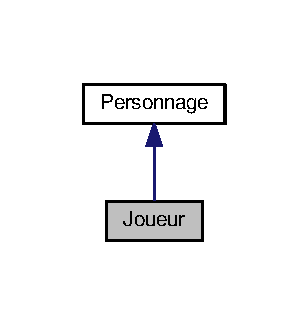
\includegraphics[width=148pt]{class_joueur__inherit__graph}
\end{center}
\end{figure}


Graphe de collaboration de Joueur\+:\nopagebreak
\begin{figure}[H]
\begin{center}
\leavevmode
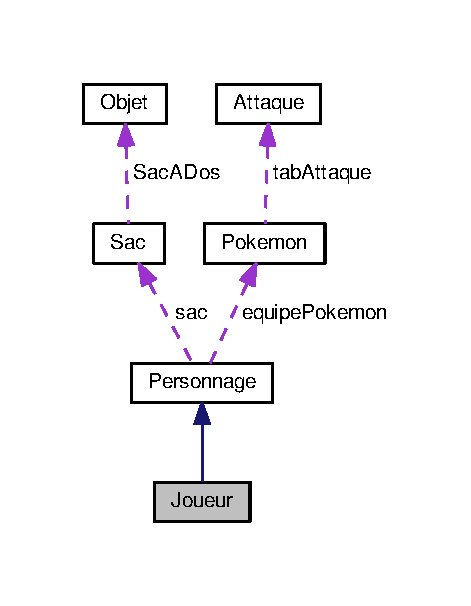
\includegraphics[width=226pt]{class_joueur__coll__graph}
\end{center}
\end{figure}
\subsection*{Fonctions membres publiques}
\begin{DoxyCompactItemize}
\item 
\mbox{\Hypertarget{class_joueur_add6c98be3020651d84f6d75ccc1d867e}\label{class_joueur_add6c98be3020651d84f6d75ccc1d867e}} 
\hyperlink{class_joueur_add6c98be3020651d84f6d75ccc1d867e}{Joueur} ()
\begin{DoxyCompactList}\small\item\em Constructeur par défaut qui appel le constructeur par défaut de \hyperlink{class_personnage}{Personnage} et qui initialise nb\+Defaites à 0,nb\+Victoires à 0,niveau à 0 et l\textquotesingle{}argent à 0. \end{DoxyCompactList}\item 
\hyperlink{class_joueur_a38f10c26b532efd5b461a1cca84f4cdd}{Joueur} (const std\+::string \&n)
\begin{DoxyCompactList}\small\item\em Constructeur qui appelle le constructeur de \hyperlink{class_personnage}{Personnage} avec un paramètre et qui initialise nb\+Defaites à 0,nb\+Victoires à 0,niveau à 0 et l\textquotesingle{}argent à 0. \end{DoxyCompactList}\item 
unsigned int \hyperlink{class_joueur_ae06420103fca19bb0dca8ba9ed261bd6}{get\+Argent} () const
\begin{DoxyCompactList}\small\item\em Accesseur de la variable argent. \end{DoxyCompactList}\item 
unsigned int \hyperlink{class_joueur_ae411355727ca5cd183183ba992693180}{get\+Nb\+Victoires} () const
\begin{DoxyCompactList}\small\item\em Accesseur de la variable nb\+Victoires. \end{DoxyCompactList}\item 
unsigned int \hyperlink{class_joueur_a82a78911f157c2fee8a7587064a4ce25}{get\+Nb\+Defaites} () const
\begin{DoxyCompactList}\small\item\em Accesseur de la variable nb\+Defaites. \end{DoxyCompactList}\item 
unsigned int \hyperlink{class_joueur_abec464c3958916f951e19ba5e12d0dbc}{get\+Niveau} () const
\begin{DoxyCompactList}\small\item\em Accesseur de la variable niveau. \end{DoxyCompactList}\item 
void \hyperlink{class_joueur_a816878a126e2e8a4610f782b4a06f53f}{recevoir\+Argent} (unsigned int n)
\begin{DoxyCompactList}\small\item\em Augmente la variable argent. \end{DoxyCompactList}\item 
void \hyperlink{class_joueur_ae496646b2078c86011fa200b631168ca}{depenser\+Argent} (unsigned int n)
\begin{DoxyCompactList}\small\item\em Diminue la variable argent. \end{DoxyCompactList}\item 
\mbox{\Hypertarget{class_joueur_a2eeebb62c0f67eabb58a4d62280675c7}\label{class_joueur_a2eeebb62c0f67eabb58a4d62280675c7}} 
void \hyperlink{class_joueur_a2eeebb62c0f67eabb58a4d62280675c7}{augmenter\+Nb\+Defaites} ()
\begin{DoxyCompactList}\small\item\em Augmente la variable nb\+Defaites de 1. \end{DoxyCompactList}\item 
\mbox{\Hypertarget{class_joueur_a8b3c0fa5871ae9320182090d22cfae69}\label{class_joueur_a8b3c0fa5871ae9320182090d22cfae69}} 
void {\bfseries set\+Niveau} (unsigned int i)
\item 
\mbox{\Hypertarget{class_joueur_a30e0e5b06537c5a7d5853230b1da9509}\label{class_joueur_a30e0e5b06537c5a7d5853230b1da9509}} 
void \hyperlink{class_joueur_a30e0e5b06537c5a7d5853230b1da9509}{augmenter\+Nb\+Victoires} ()
\begin{DoxyCompactList}\small\item\em Augemente la variable nb\+Victoires de 1. \end{DoxyCompactList}\item 
\mbox{\Hypertarget{class_joueur_afce34539fafa99280cf5976c36c1ea12}\label{class_joueur_afce34539fafa99280cf5976c36c1ea12}} 
void \hyperlink{class_joueur_afce34539fafa99280cf5976c36c1ea12}{augmenter\+Niveau} ()
\begin{DoxyCompactList}\small\item\em Augmente la variable niveau de 1. \end{DoxyCompactList}\item 
bool \hyperlink{class_joueur_a2bf2a581a2e4de27a812e21b360ab9f3}{charger\+Joueur} ()
\begin{DoxyCompactList}\small\item\em charge dans le joueur tous les informations contenues dans un fichier \end{DoxyCompactList}\item 
bool \hyperlink{class_joueur_a0bf50be14471ba0c0944b31c70bf6ad3}{sauvegarder\+Joueur} () const
\begin{DoxyCompactList}\small\item\em charge dans un fichier tout le contenu du joueur \end{DoxyCompactList}\end{DoxyCompactItemize}
\subsection*{Attributs privés}
\begin{DoxyCompactItemize}
\item 
\mbox{\Hypertarget{class_joueur_afdef85975e261b9b315e4629c5f75817}\label{class_joueur_afdef85975e261b9b315e4629c5f75817}} 
unsigned int \hyperlink{class_joueur_afdef85975e261b9b315e4629c5f75817}{nb\+Defaites}
\begin{DoxyCompactList}\small\item\em entier positif contenant le nombre de défaites du joueur \end{DoxyCompactList}\item 
\mbox{\Hypertarget{class_joueur_a64c3df68468d8c3a08ebeae05c144d7f}\label{class_joueur_a64c3df68468d8c3a08ebeae05c144d7f}} 
unsigned int \hyperlink{class_joueur_a64c3df68468d8c3a08ebeae05c144d7f}{nb\+Victoires}
\begin{DoxyCompactList}\small\item\em entier positif contenant le nombre de victoires du joueur \end{DoxyCompactList}\item 
\mbox{\Hypertarget{class_joueur_a094214899e05a45eb3807b9874fbdf66}\label{class_joueur_a094214899e05a45eb3807b9874fbdf66}} 
unsigned int \hyperlink{class_joueur_a094214899e05a45eb3807b9874fbdf66}{niveau}
\begin{DoxyCompactList}\small\item\em entier positif contenant le niveau du joueur \end{DoxyCompactList}\item 
\mbox{\Hypertarget{class_joueur_a591be8b0a344a918d728f12fefd08005}\label{class_joueur_a591be8b0a344a918d728f12fefd08005}} 
unsigned int \hyperlink{class_joueur_a591be8b0a344a918d728f12fefd08005}{argent}
\begin{DoxyCompactList}\small\item\em entier positif contenant l\textquotesingle{}argent du joueur \end{DoxyCompactList}\end{DoxyCompactItemize}


\subsection{Description détaillée}
Classe \hyperlink{class_joueur}{Joueur} hérité de la classe \hyperlink{class_personnage}{Personnage} qui gère un joueur et qui contient son nombre de défaites,de victoires,son niveau et son argent. 

\subsection{Documentation des constructeurs et destructeur}
\mbox{\Hypertarget{class_joueur_a38f10c26b532efd5b461a1cca84f4cdd}\label{class_joueur_a38f10c26b532efd5b461a1cca84f4cdd}} 
\index{Joueur@{Joueur}!Joueur@{Joueur}}
\index{Joueur@{Joueur}!Joueur@{Joueur}}
\subsubsection{\texorpdfstring{Joueur()}{Joueur()}}
{\footnotesize\ttfamily Joueur\+::\+Joueur (\begin{DoxyParamCaption}\item[{const std\+::string \&}]{n }\end{DoxyParamCaption})}



Constructeur qui appelle le constructeur de \hyperlink{class_personnage}{Personnage} avec un paramètre et qui initialise nb\+Defaites à 0,nb\+Victoires à 0,niveau à 0 et l\textquotesingle{}argent à 0. 


\begin{DoxyParams}[1]{Paramètres}
\mbox{\tt in}  & {\em n} & nom du personnage à copier \\
\hline
\end{DoxyParams}


\subsection{Documentation des fonctions membres}
\mbox{\Hypertarget{class_joueur_a2bf2a581a2e4de27a812e21b360ab9f3}\label{class_joueur_a2bf2a581a2e4de27a812e21b360ab9f3}} 
\index{Joueur@{Joueur}!charger\+Joueur@{charger\+Joueur}}
\index{charger\+Joueur@{charger\+Joueur}!Joueur@{Joueur}}
\subsubsection{\texorpdfstring{charger\+Joueur()}{chargerJoueur()}}
{\footnotesize\ttfamily bool Joueur\+::charger\+Joueur (\begin{DoxyParamCaption}{ }\end{DoxyParamCaption})}



charge dans le joueur tous les informations contenues dans un fichier 

\begin{DoxyReturn}{Renvoie}
retourne un booléen contenant 1 si le chargement c\textquotesingle{}est bien passée sinon 0 
\end{DoxyReturn}
Voici le graphe d\textquotesingle{}appel pour cette fonction \+:\nopagebreak
\begin{figure}[H]
\begin{center}
\leavevmode
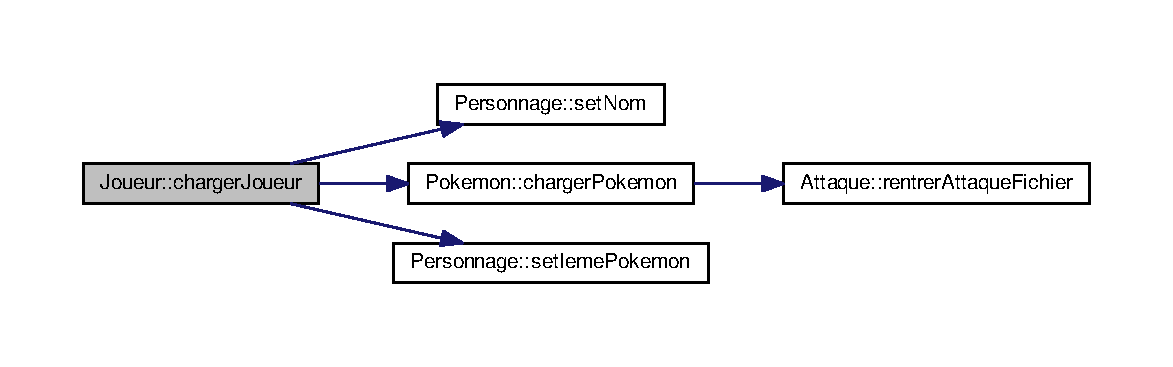
\includegraphics[width=350pt]{class_joueur_a2bf2a581a2e4de27a812e21b360ab9f3_cgraph}
\end{center}
\end{figure}
Voici le graphe des appelants de cette fonction \+:\nopagebreak
\begin{figure}[H]
\begin{center}
\leavevmode
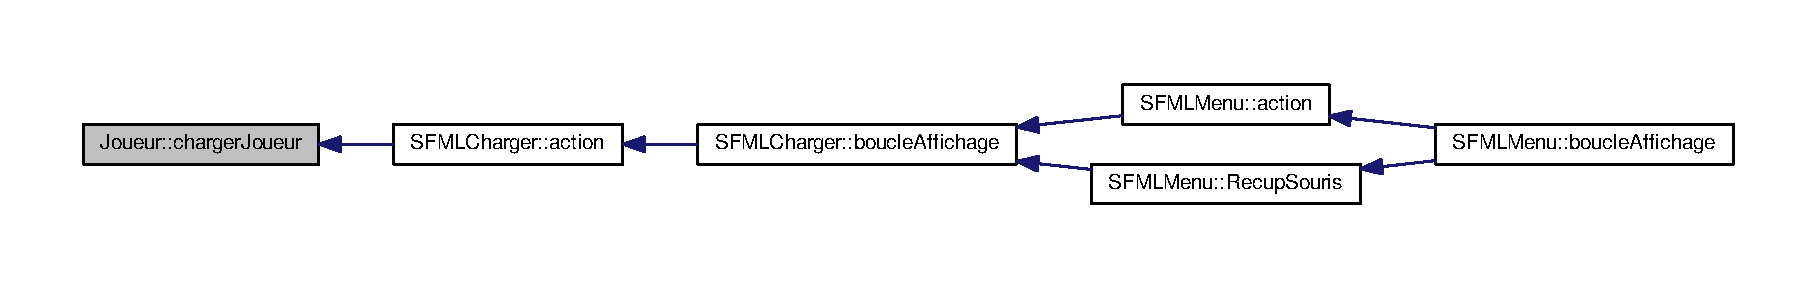
\includegraphics[width=350pt]{class_joueur_a2bf2a581a2e4de27a812e21b360ab9f3_icgraph}
\end{center}
\end{figure}
\mbox{\Hypertarget{class_joueur_ae496646b2078c86011fa200b631168ca}\label{class_joueur_ae496646b2078c86011fa200b631168ca}} 
\index{Joueur@{Joueur}!depenser\+Argent@{depenser\+Argent}}
\index{depenser\+Argent@{depenser\+Argent}!Joueur@{Joueur}}
\subsubsection{\texorpdfstring{depenser\+Argent()}{depenserArgent()}}
{\footnotesize\ttfamily void Joueur\+::depenser\+Argent (\begin{DoxyParamCaption}\item[{unsigned int}]{n }\end{DoxyParamCaption})}



Diminue la variable argent. 


\begin{DoxyParams}[1]{Paramètres}
\mbox{\tt in}  & {\em n} & entier postif contenant l\textquotesingle{}argent à enlever \\
\hline
\end{DoxyParams}
\mbox{\Hypertarget{class_joueur_ae06420103fca19bb0dca8ba9ed261bd6}\label{class_joueur_ae06420103fca19bb0dca8ba9ed261bd6}} 
\index{Joueur@{Joueur}!get\+Argent@{get\+Argent}}
\index{get\+Argent@{get\+Argent}!Joueur@{Joueur}}
\subsubsection{\texorpdfstring{get\+Argent()}{getArgent()}}
{\footnotesize\ttfamily unsigned int Joueur\+::get\+Argent (\begin{DoxyParamCaption}{ }\end{DoxyParamCaption}) const}



Accesseur de la variable argent. 

\begin{DoxyReturn}{Renvoie}
retourne un entier positif contenant l\textquotesingle{}argent du joueur 
\end{DoxyReturn}
\mbox{\Hypertarget{class_joueur_a82a78911f157c2fee8a7587064a4ce25}\label{class_joueur_a82a78911f157c2fee8a7587064a4ce25}} 
\index{Joueur@{Joueur}!get\+Nb\+Defaites@{get\+Nb\+Defaites}}
\index{get\+Nb\+Defaites@{get\+Nb\+Defaites}!Joueur@{Joueur}}
\subsubsection{\texorpdfstring{get\+Nb\+Defaites()}{getNbDefaites()}}
{\footnotesize\ttfamily unsigned int Joueur\+::get\+Nb\+Defaites (\begin{DoxyParamCaption}{ }\end{DoxyParamCaption}) const}



Accesseur de la variable nb\+Defaites. 

\begin{DoxyReturn}{Renvoie}
retourne un entier positif contenant le nombre de défaites du joueur 
\end{DoxyReturn}
\mbox{\Hypertarget{class_joueur_ae411355727ca5cd183183ba992693180}\label{class_joueur_ae411355727ca5cd183183ba992693180}} 
\index{Joueur@{Joueur}!get\+Nb\+Victoires@{get\+Nb\+Victoires}}
\index{get\+Nb\+Victoires@{get\+Nb\+Victoires}!Joueur@{Joueur}}
\subsubsection{\texorpdfstring{get\+Nb\+Victoires()}{getNbVictoires()}}
{\footnotesize\ttfamily unsigned int Joueur\+::get\+Nb\+Victoires (\begin{DoxyParamCaption}{ }\end{DoxyParamCaption}) const}



Accesseur de la variable nb\+Victoires. 

\begin{DoxyReturn}{Renvoie}
retourne un entier positif contenant le nombre de victoires du joueur 
\end{DoxyReturn}
\mbox{\Hypertarget{class_joueur_abec464c3958916f951e19ba5e12d0dbc}\label{class_joueur_abec464c3958916f951e19ba5e12d0dbc}} 
\index{Joueur@{Joueur}!get\+Niveau@{get\+Niveau}}
\index{get\+Niveau@{get\+Niveau}!Joueur@{Joueur}}
\subsubsection{\texorpdfstring{get\+Niveau()}{getNiveau()}}
{\footnotesize\ttfamily unsigned int Joueur\+::get\+Niveau (\begin{DoxyParamCaption}{ }\end{DoxyParamCaption}) const}



Accesseur de la variable niveau. 

\begin{DoxyReturn}{Renvoie}
retourne un entier positif contenant le niveau du joueur 
\end{DoxyReturn}
Voici le graphe des appelants de cette fonction \+:\nopagebreak
\begin{figure}[H]
\begin{center}
\leavevmode
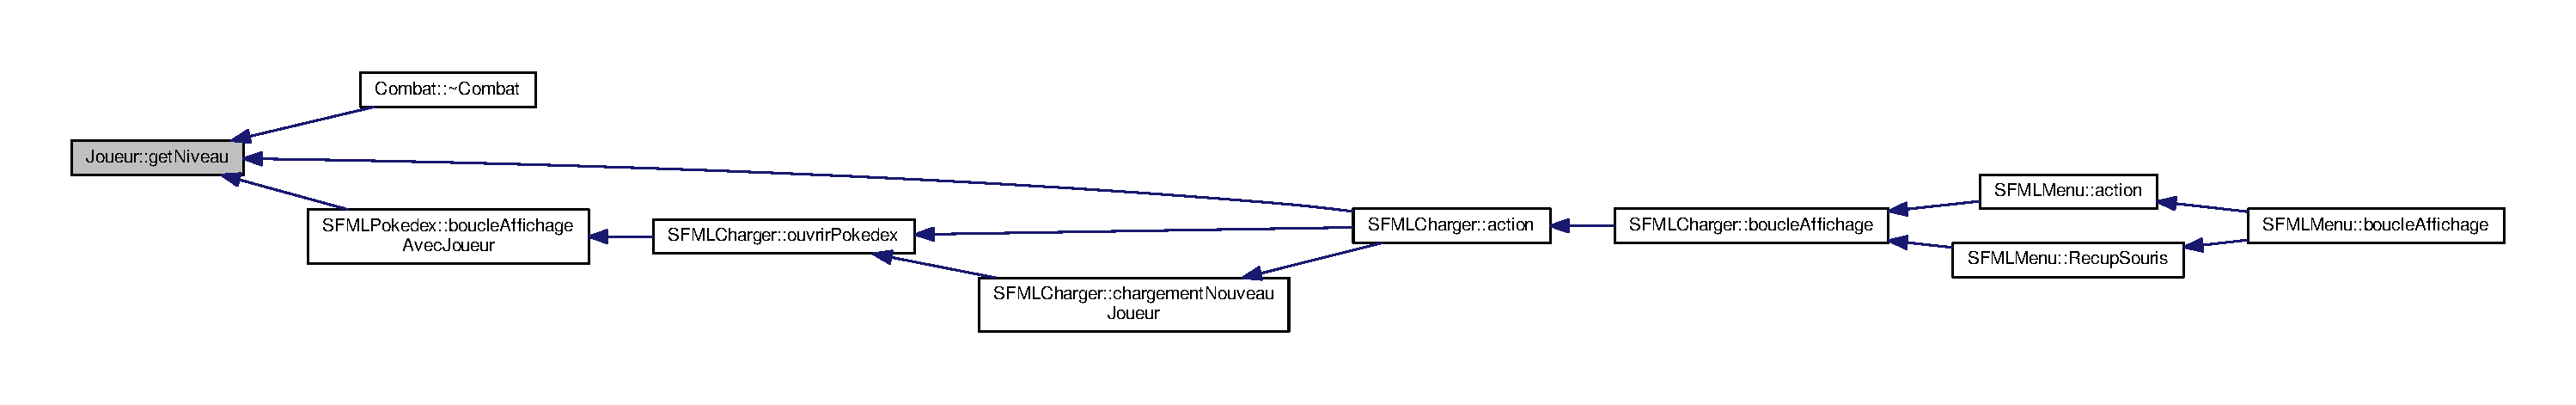
\includegraphics[width=350pt]{class_joueur_abec464c3958916f951e19ba5e12d0dbc_icgraph}
\end{center}
\end{figure}
\mbox{\Hypertarget{class_joueur_a816878a126e2e8a4610f782b4a06f53f}\label{class_joueur_a816878a126e2e8a4610f782b4a06f53f}} 
\index{Joueur@{Joueur}!recevoir\+Argent@{recevoir\+Argent}}
\index{recevoir\+Argent@{recevoir\+Argent}!Joueur@{Joueur}}
\subsubsection{\texorpdfstring{recevoir\+Argent()}{recevoirArgent()}}
{\footnotesize\ttfamily void Joueur\+::recevoir\+Argent (\begin{DoxyParamCaption}\item[{unsigned int}]{n }\end{DoxyParamCaption})}



Augmente la variable argent. 


\begin{DoxyParams}[1]{Paramètres}
\mbox{\tt in}  & {\em n} & entier postif contenant l\textquotesingle{}argent à ajouter \\
\hline
\end{DoxyParams}
\mbox{\Hypertarget{class_joueur_a0bf50be14471ba0c0944b31c70bf6ad3}\label{class_joueur_a0bf50be14471ba0c0944b31c70bf6ad3}} 
\index{Joueur@{Joueur}!sauvegarder\+Joueur@{sauvegarder\+Joueur}}
\index{sauvegarder\+Joueur@{sauvegarder\+Joueur}!Joueur@{Joueur}}
\subsubsection{\texorpdfstring{sauvegarder\+Joueur()}{sauvegarderJoueur()}}
{\footnotesize\ttfamily bool Joueur\+::sauvegarder\+Joueur (\begin{DoxyParamCaption}{ }\end{DoxyParamCaption}) const}



charge dans un fichier tout le contenu du joueur 

\begin{DoxyReturn}{Renvoie}
retourne un booléen contenant 1 si la sauvergarde c\textquotesingle{}est bien passée sinon 0 
\end{DoxyReturn}
Voici le graphe d\textquotesingle{}appel pour cette fonction \+:\nopagebreak
\begin{figure}[H]
\begin{center}
\leavevmode
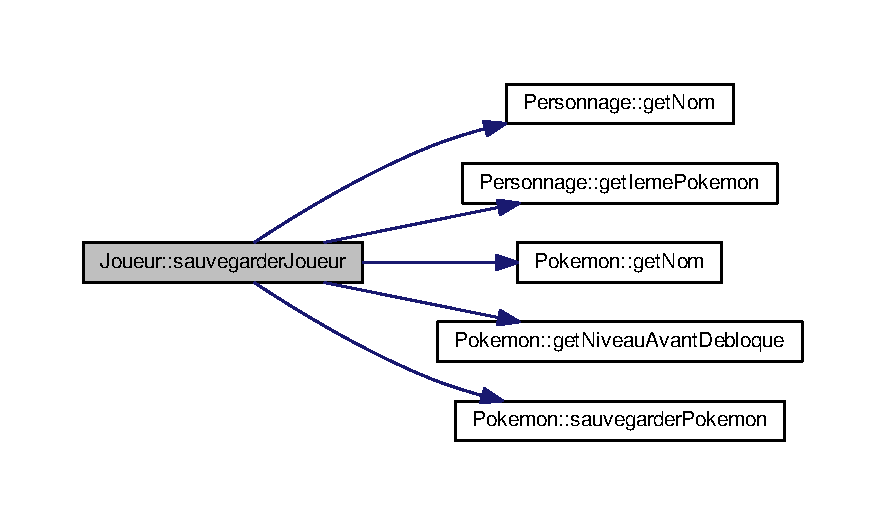
\includegraphics[width=350pt]{class_joueur_a0bf50be14471ba0c0944b31c70bf6ad3_cgraph}
\end{center}
\end{figure}
Voici le graphe des appelants de cette fonction \+:\nopagebreak
\begin{figure}[H]
\begin{center}
\leavevmode
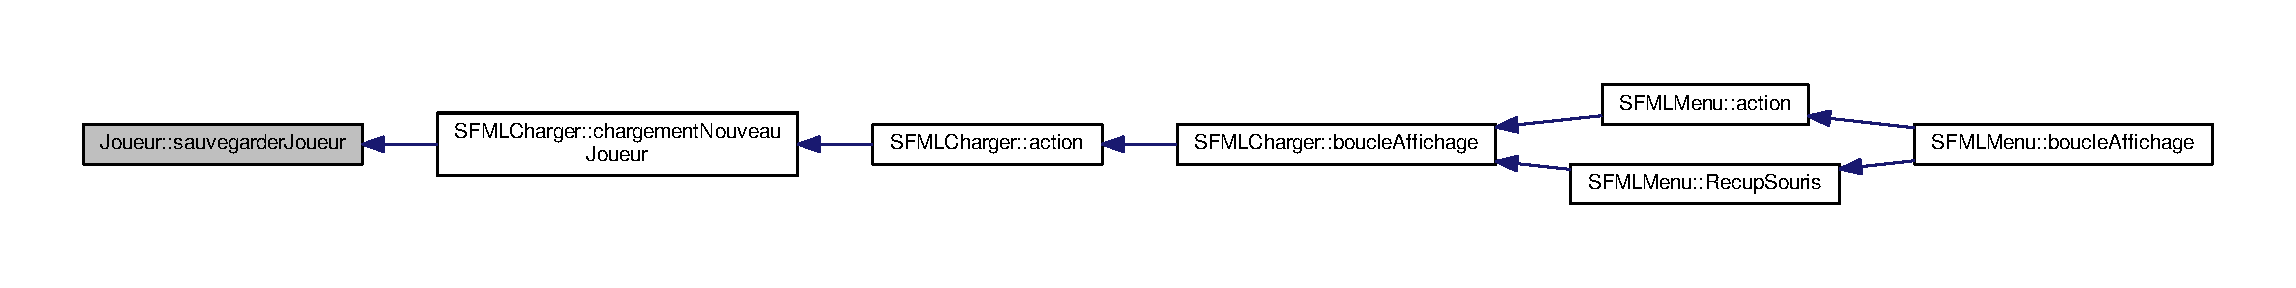
\includegraphics[width=350pt]{class_joueur_a0bf50be14471ba0c0944b31c70bf6ad3_icgraph}
\end{center}
\end{figure}


La documentation de cette classe a été générée à partir des fichiers suivants \+:\begin{DoxyCompactItemize}
\item 
/home/corentin/\+Documents/lifap4/src/\+Personnage/\hyperlink{_personnage_8h}{Personnage.\+h}\item 
/home/corentin/\+Documents/lifap4/src/\+Personnage/\hyperlink{_personnage_8cpp}{Personnage.\+cpp}\end{DoxyCompactItemize}

\hypertarget{class_objet}{}\section{Référence de la classe Objet}
\label{class_objet}\index{Objet@{Objet}}


Classe \hyperlink{class_objet}{Objet} qui gère un objet et qui contient son type d\textquotesingle{}objet,son nom,sa description et sa quantité  




{\ttfamily \#include $<$Objet.\+h$>$}

\subsection*{Fonctions membres publiques}
\begin{DoxyCompactItemize}
\item 
\mbox{\Hypertarget{class_objet_aefdd826d50085897e4894ffef4597d04}\label{class_objet_aefdd826d50085897e4894ffef4597d04}} 
\hyperlink{class_objet_aefdd826d50085897e4894ffef4597d04}{Objet} ()
\begin{DoxyCompactList}\small\item\em Constructeur par défaut qui initialise le type d\textquotesingle{}objet à Default, le nom\+Objet à \char`\"{}\+N\+U\+L\+L\char`\"{}, la description à \char`\"{}\+Aucune description\char`\"{} et la quantite à 0. \end{DoxyCompactList}\item 
int \hyperlink{class_objet_ab75ba7bf1170582a4d50ba8848be2848}{get\+Type\+Objet} () const
\begin{DoxyCompactList}\small\item\em Accesseur de la variable Type\+Objet. \end{DoxyCompactList}\item 
std\+::string \hyperlink{class_objet_a29be0a2d83cdebac4fedd495e3824515}{get\+Nom\+Objet} () const
\begin{DoxyCompactList}\small\item\em Accesseur de la variable nom\+Objet. \end{DoxyCompactList}\item 
unsigned int \hyperlink{class_objet_a3352afeefcae6415b3c73112fd588ab5}{get\+Quantite} () const
\begin{DoxyCompactList}\small\item\em Accesseur de la variable quantite. \end{DoxyCompactList}\item 
void \hyperlink{class_objet_a2183a02ee228f3ba1e52e0e5b9904dce}{set\+Type\+Objet} (const Type\+Objet \&type)
\begin{DoxyCompactList}\small\item\em Mutateur de la variable type\+Objet. \end{DoxyCompactList}\item 
void \hyperlink{class_objet_a666418b066069a2a5e35f88dc1f77f0f}{set\+Nom\+Objet} (const std\+::string \&nom)
\begin{DoxyCompactList}\small\item\em Mutateur de la variable nom\+Objet. \end{DoxyCompactList}\item 
void \hyperlink{class_objet_a92eac9151b39f0a03a94ba02f25018c9}{set\+Quantite} (unsigned int nombre)
\begin{DoxyCompactList}\small\item\em Mutateur de la variable quantite. \end{DoxyCompactList}\item 
\hyperlink{class_objet}{Objet} \& \hyperlink{class_objet_a9e4b0fb73f3a95425f0239c91c7513f4}{operator=} (const \hyperlink{class_objet}{Objet} \&objet)
\begin{DoxyCompactList}\small\item\em surcharge de l\textquotesingle{}opérateur égal \end{DoxyCompactList}\item 
\mbox{\Hypertarget{class_objet_aa39f9e7546969cc0a53a2412deb4d27a}\label{class_objet_aa39f9e7546969cc0a53a2412deb4d27a}} 
void \hyperlink{class_objet_aa39f9e7546969cc0a53a2412deb4d27a}{baisser\+Quantite} ()
\begin{DoxyCompactList}\small\item\em baisse la quantité de l\textquotesingle{}objet de un \end{DoxyCompactList}\item 
\mbox{\Hypertarget{class_objet_a1e7b9c9e5cc9417b182258bcb7a0ae21}\label{class_objet_a1e7b9c9e5cc9417b182258bcb7a0ae21}} 
void \hyperlink{class_objet_a1e7b9c9e5cc9417b182258bcb7a0ae21}{test\+Regression} ()
\begin{DoxyCompactList}\small\item\em test toutes les fonctions de la classe \end{DoxyCompactList}\end{DoxyCompactItemize}
\subsection*{Attributs privés}
\begin{DoxyCompactItemize}
\item 
\mbox{\Hypertarget{class_objet_a7561dbf89b5c4e9262198c502c070642}\label{class_objet_a7561dbf89b5c4e9262198c502c070642}} 
Type\+Objet \hyperlink{class_objet_a7561dbf89b5c4e9262198c502c070642}{type\+Objet}
\begin{DoxyCompactList}\small\item\em enum Type\+Objet contenant le type de l\textquotesingle{}objet (entre -\/1 et 15) \end{DoxyCompactList}\item 
\mbox{\Hypertarget{class_objet_a958a8478200ad06343102d7709643e5c}\label{class_objet_a958a8478200ad06343102d7709643e5c}} 
std\+::string \hyperlink{class_objet_a958a8478200ad06343102d7709643e5c}{nom\+Objet}
\begin{DoxyCompactList}\small\item\em chaîne de caractère contenant le nom de l\textquotesingle{}objet \end{DoxyCompactList}\item 
\mbox{\Hypertarget{class_objet_a8ab48702d757dbea52a03aa0d4de9de9}\label{class_objet_a8ab48702d757dbea52a03aa0d4de9de9}} 
unsigned int \hyperlink{class_objet_a8ab48702d757dbea52a03aa0d4de9de9}{quantite}
\begin{DoxyCompactList}\small\item\em entier positif contenant la quantité de l\textquotesingle{}objet \end{DoxyCompactList}\end{DoxyCompactItemize}


\subsection{Description détaillée}
Classe \hyperlink{class_objet}{Objet} qui gère un objet et qui contient son type d\textquotesingle{}objet,son nom,sa description et sa quantité 

\subsection{Documentation des fonctions membres}
\mbox{\Hypertarget{class_objet_a29be0a2d83cdebac4fedd495e3824515}\label{class_objet_a29be0a2d83cdebac4fedd495e3824515}} 
\index{Objet@{Objet}!get\+Nom\+Objet@{get\+Nom\+Objet}}
\index{get\+Nom\+Objet@{get\+Nom\+Objet}!Objet@{Objet}}
\subsubsection{\texorpdfstring{get\+Nom\+Objet()}{getNomObjet()}}
{\footnotesize\ttfamily std\+::string Objet\+::get\+Nom\+Objet (\begin{DoxyParamCaption}{ }\end{DoxyParamCaption}) const}



Accesseur de la variable nom\+Objet. 

\begin{DoxyReturn}{Renvoie}
retourne une chaîne de caractère contenant le nom de l\textquotesingle{}objet 
\end{DoxyReturn}
Voici le graphe des appelants de cette fonction \+:\nopagebreak
\begin{figure}[H]
\begin{center}
\leavevmode
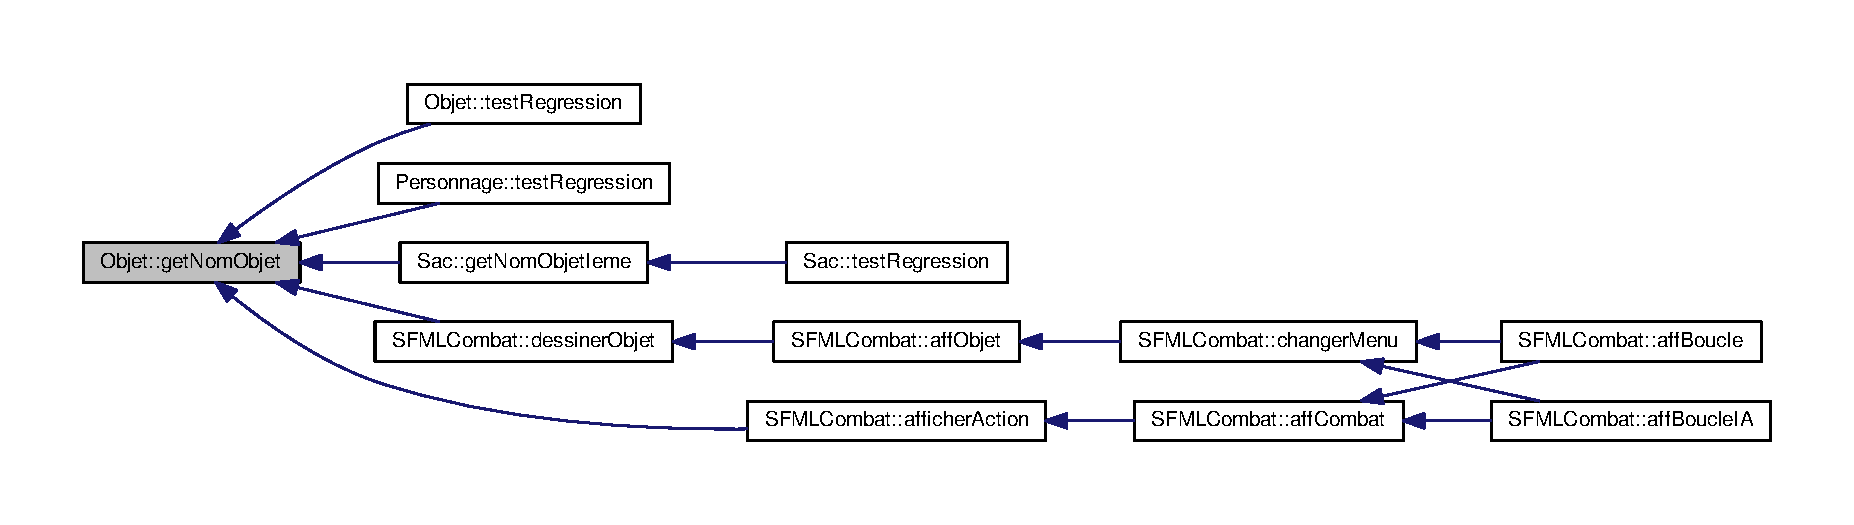
\includegraphics[width=350pt]{class_objet_a29be0a2d83cdebac4fedd495e3824515_icgraph}
\end{center}
\end{figure}
\mbox{\Hypertarget{class_objet_a3352afeefcae6415b3c73112fd588ab5}\label{class_objet_a3352afeefcae6415b3c73112fd588ab5}} 
\index{Objet@{Objet}!get\+Quantite@{get\+Quantite}}
\index{get\+Quantite@{get\+Quantite}!Objet@{Objet}}
\subsubsection{\texorpdfstring{get\+Quantite()}{getQuantite()}}
{\footnotesize\ttfamily unsigned int Objet\+::get\+Quantite (\begin{DoxyParamCaption}{ }\end{DoxyParamCaption}) const}



Accesseur de la variable quantite. 

\begin{DoxyReturn}{Renvoie}
retourne un entier positif contenant la quantité de l\textquotesingle{}objet 
\end{DoxyReturn}
Voici le graphe des appelants de cette fonction \+:\nopagebreak
\begin{figure}[H]
\begin{center}
\leavevmode
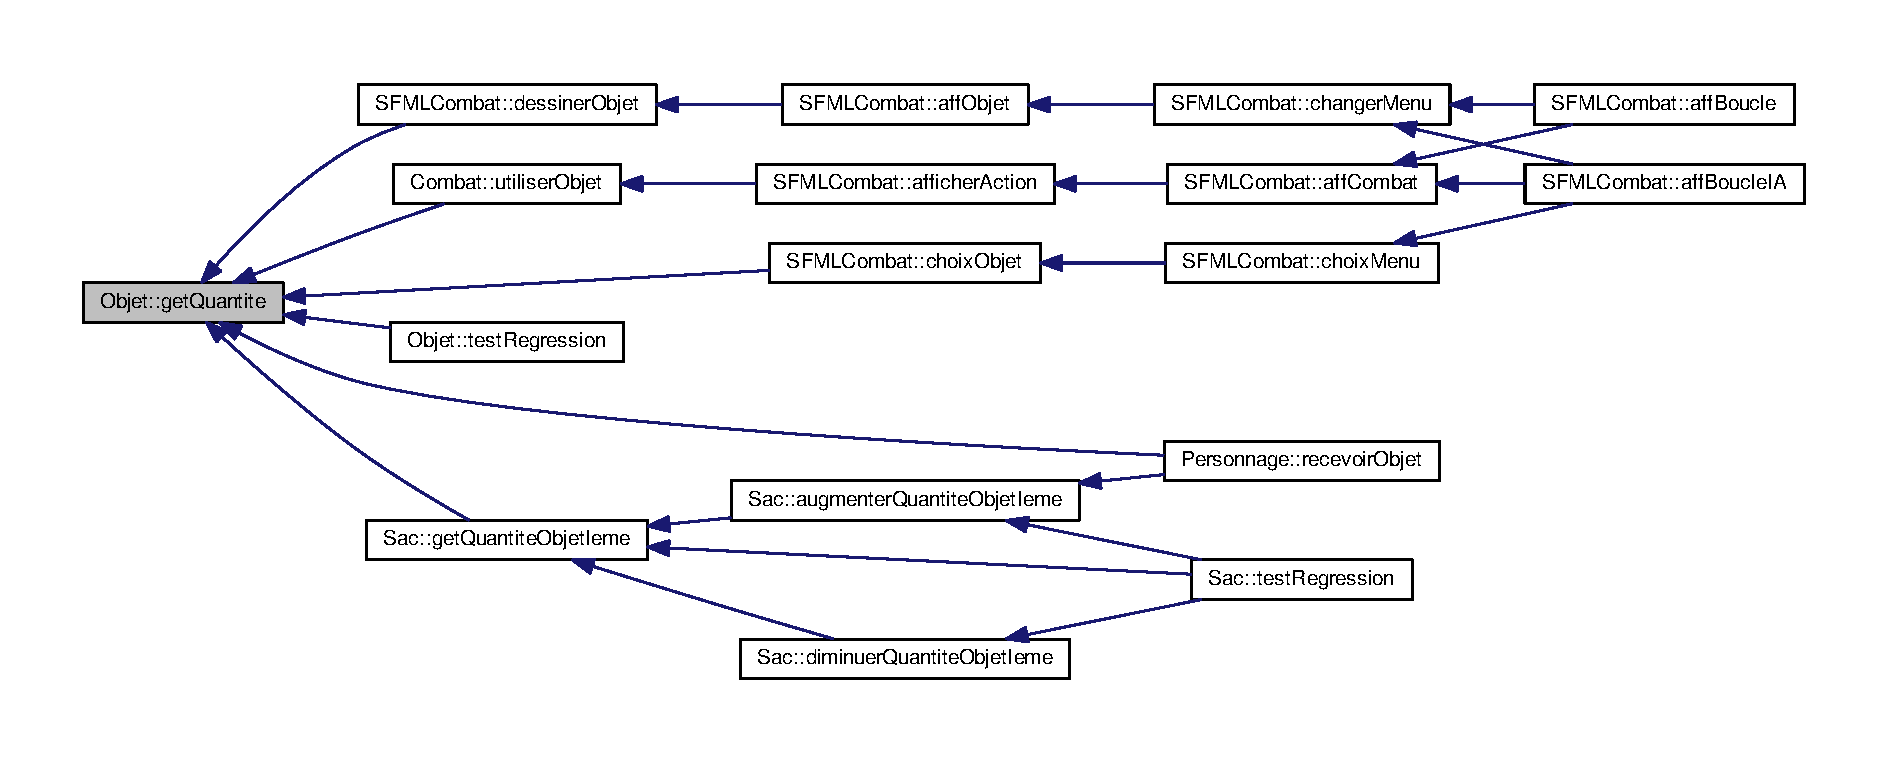
\includegraphics[width=350pt]{class_objet_a3352afeefcae6415b3c73112fd588ab5_icgraph}
\end{center}
\end{figure}
\mbox{\Hypertarget{class_objet_ab75ba7bf1170582a4d50ba8848be2848}\label{class_objet_ab75ba7bf1170582a4d50ba8848be2848}} 
\index{Objet@{Objet}!get\+Type\+Objet@{get\+Type\+Objet}}
\index{get\+Type\+Objet@{get\+Type\+Objet}!Objet@{Objet}}
\subsubsection{\texorpdfstring{get\+Type\+Objet()}{getTypeObjet()}}
{\footnotesize\ttfamily int Objet\+::get\+Type\+Objet (\begin{DoxyParamCaption}{ }\end{DoxyParamCaption}) const}



Accesseur de la variable Type\+Objet. 

\begin{DoxyReturn}{Renvoie}
retourne en entier contenant le type de l\textquotesingle{}objet 
\end{DoxyReturn}
Voici le graphe des appelants de cette fonction \+:\nopagebreak
\begin{figure}[H]
\begin{center}
\leavevmode
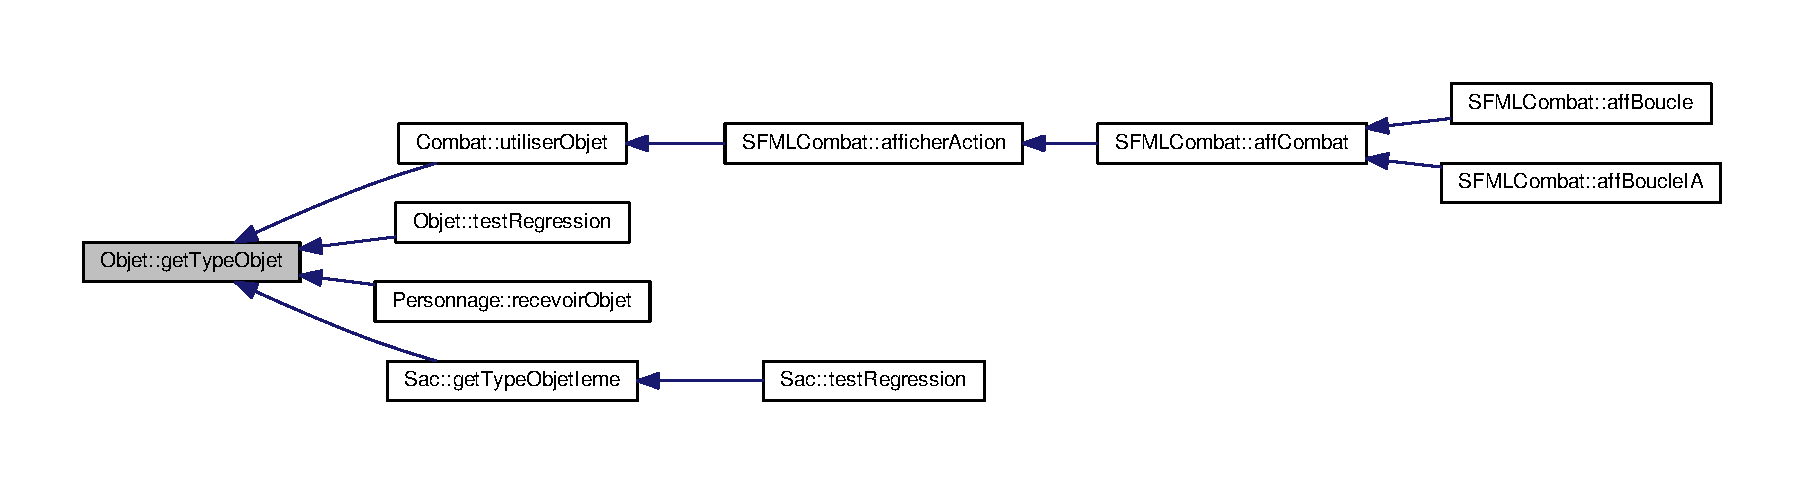
\includegraphics[width=350pt]{class_objet_ab75ba7bf1170582a4d50ba8848be2848_icgraph}
\end{center}
\end{figure}
\mbox{\Hypertarget{class_objet_a9e4b0fb73f3a95425f0239c91c7513f4}\label{class_objet_a9e4b0fb73f3a95425f0239c91c7513f4}} 
\index{Objet@{Objet}!operator=@{operator=}}
\index{operator=@{operator=}!Objet@{Objet}}
\subsubsection{\texorpdfstring{operator=()}{operator=()}}
{\footnotesize\ttfamily \hyperlink{class_objet}{Objet} \& Objet\+::operator= (\begin{DoxyParamCaption}\item[{const \hyperlink{class_objet}{Objet} \&}]{objet }\end{DoxyParamCaption})}



surcharge de l\textquotesingle{}opérateur égal 


\begin{DoxyParams}[1]{Paramètres}
\mbox{\tt in}  & {\em objet} & \hyperlink{class_objet}{Objet} contenant l\textquotesingle{}objet à copier \\
\hline
\end{DoxyParams}
\begin{DoxyReturn}{Renvoie}
retourne une réference sur l\textquotesingle{}instance objet 
\end{DoxyReturn}
\mbox{\Hypertarget{class_objet_a666418b066069a2a5e35f88dc1f77f0f}\label{class_objet_a666418b066069a2a5e35f88dc1f77f0f}} 
\index{Objet@{Objet}!set\+Nom\+Objet@{set\+Nom\+Objet}}
\index{set\+Nom\+Objet@{set\+Nom\+Objet}!Objet@{Objet}}
\subsubsection{\texorpdfstring{set\+Nom\+Objet()}{setNomObjet()}}
{\footnotesize\ttfamily void Objet\+::set\+Nom\+Objet (\begin{DoxyParamCaption}\item[{const std\+::string \&}]{nom }\end{DoxyParamCaption})}



Mutateur de la variable nom\+Objet. 


\begin{DoxyParams}[1]{Paramètres}
\mbox{\tt in}  & {\em nom} & chaîne de caractère contenant le nom de l\textquotesingle{}objet à copier \\
\hline
\end{DoxyParams}
Voici le graphe des appelants de cette fonction \+:\nopagebreak
\begin{figure}[H]
\begin{center}
\leavevmode
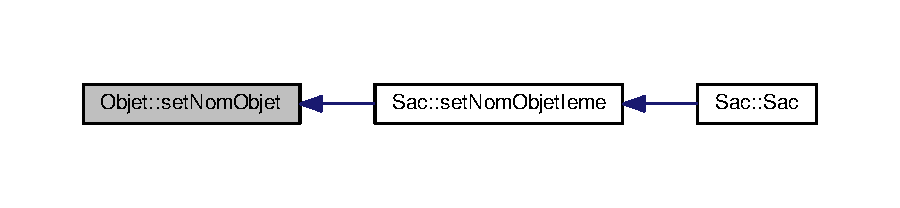
\includegraphics[width=350pt]{class_objet_a666418b066069a2a5e35f88dc1f77f0f_icgraph}
\end{center}
\end{figure}
\mbox{\Hypertarget{class_objet_a92eac9151b39f0a03a94ba02f25018c9}\label{class_objet_a92eac9151b39f0a03a94ba02f25018c9}} 
\index{Objet@{Objet}!set\+Quantite@{set\+Quantite}}
\index{set\+Quantite@{set\+Quantite}!Objet@{Objet}}
\subsubsection{\texorpdfstring{set\+Quantite()}{setQuantite()}}
{\footnotesize\ttfamily void Objet\+::set\+Quantite (\begin{DoxyParamCaption}\item[{unsigned int}]{nombre }\end{DoxyParamCaption})}



Mutateur de la variable quantite. 


\begin{DoxyParams}[1]{Paramètres}
\mbox{\tt in}  & {\em nombre} & entier positif contenant la quantité de l\textquotesingle{}objet à copier \\
\hline
\end{DoxyParams}
Voici le graphe des appelants de cette fonction \+:\nopagebreak
\begin{figure}[H]
\begin{center}
\leavevmode
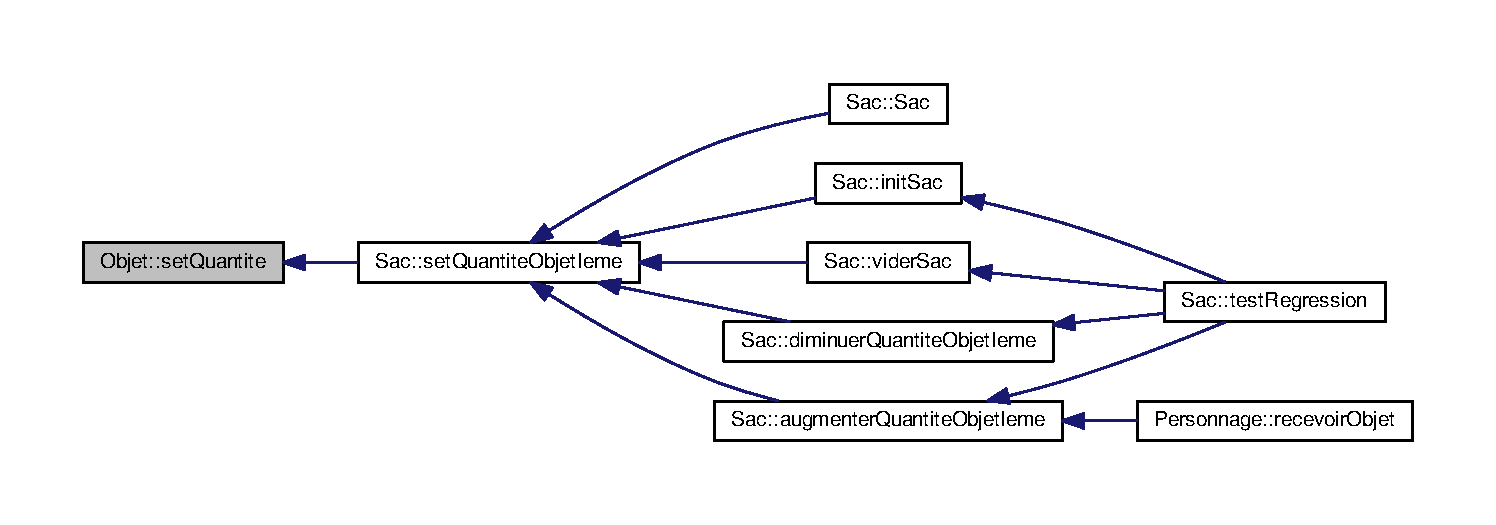
\includegraphics[width=350pt]{class_objet_a92eac9151b39f0a03a94ba02f25018c9_icgraph}
\end{center}
\end{figure}
\mbox{\Hypertarget{class_objet_a2183a02ee228f3ba1e52e0e5b9904dce}\label{class_objet_a2183a02ee228f3ba1e52e0e5b9904dce}} 
\index{Objet@{Objet}!set\+Type\+Objet@{set\+Type\+Objet}}
\index{set\+Type\+Objet@{set\+Type\+Objet}!Objet@{Objet}}
\subsubsection{\texorpdfstring{set\+Type\+Objet()}{setTypeObjet()}}
{\footnotesize\ttfamily void Objet\+::set\+Type\+Objet (\begin{DoxyParamCaption}\item[{const Type\+Objet \&}]{type }\end{DoxyParamCaption})}



Mutateur de la variable type\+Objet. 


\begin{DoxyParams}[1]{Paramètres}
\mbox{\tt in}  & {\em type} & type de l\textquotesingle{}objet à copier \\
\hline
\end{DoxyParams}
Voici le graphe des appelants de cette fonction \+:\nopagebreak
\begin{figure}[H]
\begin{center}
\leavevmode
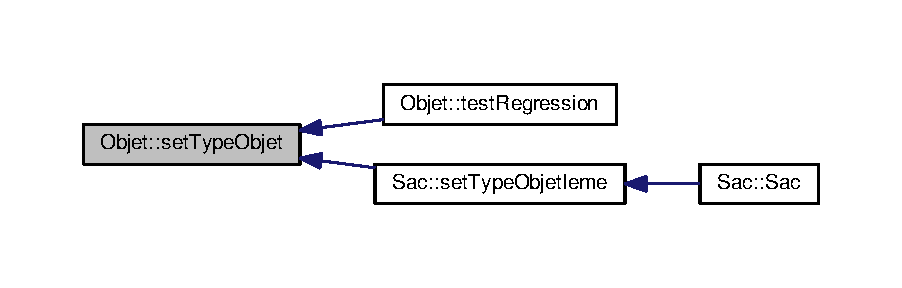
\includegraphics[width=350pt]{class_objet_a2183a02ee228f3ba1e52e0e5b9904dce_icgraph}
\end{center}
\end{figure}


La documentation de cette classe a été générée à partir des fichiers suivants \+:\begin{DoxyCompactItemize}
\item 
/home/corentin/\+Documents/lifap4/src/\+Objet/\hyperlink{_objet_8h}{Objet.\+h}\item 
/home/corentin/\+Documents/lifap4/src/\+Objet/\hyperlink{_objet_8cpp}{Objet.\+cpp}\end{DoxyCompactItemize}

\hypertarget{class_personnage}{}\section{Personnage Class Reference}
\label{class_personnage}\index{Personnage@{Personnage}}


Inheritance diagram for Personnage\+:
\nopagebreak
\begin{figure}[H]
\begin{center}
\leavevmode
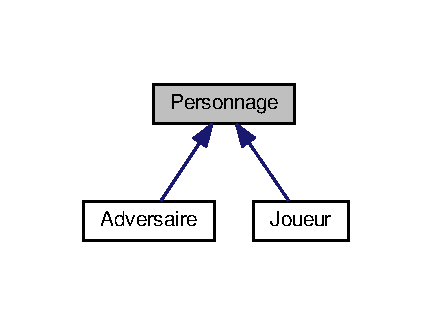
\includegraphics[width=208pt]{class_personnage__inherit__graph}
\end{center}
\end{figure}
\subsection*{Public Member Functions}
\begin{DoxyCompactItemize}
\item 
\mbox{\Hypertarget{class_personnage_a8ed6fad2f650ba45a3cf3586cbd1d1b7}\label{class_personnage_a8ed6fad2f650ba45a3cf3586cbd1d1b7}} 
{\bfseries Personnage} (const std\+::string \&n, const std\+::string \&d, char s)
\item 
\mbox{\Hypertarget{class_personnage_a411597dd00afced2f6eeb70461833dbe}\label{class_personnage_a411597dd00afced2f6eeb70461833dbe}} 
std\+::string {\bfseries get\+Nom} () const
\item 
\mbox{\Hypertarget{class_personnage_a3ca6a49bfbf0edc453dd1ae82d95ae71}\label{class_personnage_a3ca6a49bfbf0edc453dd1ae82d95ae71}} 
std\+::string {\bfseries get\+Dialogue} () const
\item 
\mbox{\Hypertarget{class_personnage_a07a28601294de4135b3d8721bc560ed8}\label{class_personnage_a07a28601294de4135b3d8721bc560ed8}} 
char {\bfseries get\+Sexe} () const
\item 
\mbox{\Hypertarget{class_personnage_abd45dd4e1a4099a6300c037fc41e1037}\label{class_personnage_abd45dd4e1a4099a6300c037fc41e1037}} 
\hyperlink{class_pokemon}{Pokemon} {\bfseries get\+Ieme\+Pokemon} (unsigned int i) const
\item 
\mbox{\Hypertarget{class_personnage_aeab0448ba1e833d57ee17827e3a6ac0d}\label{class_personnage_aeab0448ba1e833d57ee17827e3a6ac0d}} 
\hyperlink{class_pokemon}{Pokemon} $\ast$ {\bfseries get\+Ieme\+Pokemon\+Ref} (unsigned int i)
\item 
\mbox{\Hypertarget{class_personnage_a853a057817adeacdf048534cf30254d2}\label{class_personnage_a853a057817adeacdf048534cf30254d2}} 
\hyperlink{class_pokemon}{Pokemon} $\ast$ {\bfseries get\+Equipe\+Pokemon} ()
\item 
\mbox{\Hypertarget{class_personnage_a32cf123b507c36c8adbf9bd22cb0b9a2}\label{class_personnage_a32cf123b507c36c8adbf9bd22cb0b9a2}} 
\hyperlink{class_objet}{Objet} {\bfseries get\+Objet\+Dans\+Sac} (unsigned int i) const
\item 
\mbox{\Hypertarget{class_personnage_a6b3462a550a38c9e9163495c2b2015f4}\label{class_personnage_a6b3462a550a38c9e9163495c2b2015f4}} 
\hyperlink{class_objet}{Objet} $\ast$ {\bfseries get\+Objet\+Dans\+Sac\+Ref} (unsigned int i)
\item 
\mbox{\Hypertarget{class_personnage_aa6dd3ce808644f01d0cdb891f67e896c}\label{class_personnage_aa6dd3ce808644f01d0cdb891f67e896c}} 
\hyperlink{class_sac}{Sac} {\bfseries get\+Sac} () const
\item 
\mbox{\Hypertarget{class_personnage_acb7d9ff9b6b6753b8c93fae58f428db1}\label{class_personnage_acb7d9ff9b6b6753b8c93fae58f428db1}} 
\hyperlink{class_sac}{Sac} $\ast$ {\bfseries get\+Sac\+Ref} ()
\item 
\mbox{\Hypertarget{class_personnage_a46d6d6f6f9b647c04c1cad509bec0935}\label{class_personnage_a46d6d6f6f9b647c04c1cad509bec0935}} 
void {\bfseries set\+Nom} (const std\+::string \&n)
\item 
\mbox{\Hypertarget{class_personnage_af72b99d62adf0fa6bda389bc58fdcd7d}\label{class_personnage_af72b99d62adf0fa6bda389bc58fdcd7d}} 
void {\bfseries set\+Dialogue} (const std\+::string \&d)
\item 
\mbox{\Hypertarget{class_personnage_ae9e94e72e002695ae1461aa538e5e880}\label{class_personnage_ae9e94e72e002695ae1461aa538e5e880}} 
void {\bfseries set\+Ieme\+Pokemon} (const \hyperlink{class_pokemon}{Pokemon} \&pokemon, unsigned int i)
\item 
\mbox{\Hypertarget{class_personnage_a862b4dd5006dec4d542550b1a1e308db}\label{class_personnage_a862b4dd5006dec4d542550b1a1e308db}} 
void {\bfseries set\+Sexe} (char s)
\item 
\mbox{\Hypertarget{class_personnage_a70fb0f0180dd625cf96dfc469ae5710e}\label{class_personnage_a70fb0f0180dd625cf96dfc469ae5710e}} 
void {\bfseries recevoir\+Objet} (const \hyperlink{class_objet}{Objet} \&objet)
\item 
\mbox{\Hypertarget{class_personnage_a8b827a72e42d38de1b6d29dee145a4b5}\label{class_personnage_a8b827a72e42d38de1b6d29dee145a4b5}} 
void {\bfseries test\+Regression} ()
\item 
\mbox{\Hypertarget{class_personnage_a6727627eb37382d3d8f12514551df9bd}\label{class_personnage_a6727627eb37382d3d8f12514551df9bd}} 
\hyperlink{class_personnage}{Personnage} \& {\bfseries operator=} (const \hyperlink{class_personnage}{Personnage} \&Perso)
\end{DoxyCompactItemize}


The documentation for this class was generated from the following files\+:\begin{DoxyCompactItemize}
\item 
/home/corentin/\+Documents/lifap4/src/\+Personnage/Personnage.\+h\item 
/home/corentin/\+Documents/lifap4/src/\+Personnage/Personnage.\+cpp\end{DoxyCompactItemize}

\hypertarget{class_pokemon}{}\section{Pokemon Class Reference}
\label{class_pokemon}\index{Pokemon@{Pokemon}}
\subsection*{Public Member Functions}
\begin{DoxyCompactItemize}
\item 
\mbox{\Hypertarget{class_pokemon_a29848dd8e04d070a2927b9beeca8d47c}\label{class_pokemon_a29848dd8e04d070a2927b9beeca8d47c}} 
{\bfseries Pokemon} (const std \+::string \&nom\+Pokemon, unsigned int i, unsigned int defense\+Spe, unsigned int defense\+Phy, unsigned int attaque\+Spe, unsigned int attaque\+Phy, unsigned int vit, unsigned int P\+V\+Pokemon, const int \&type1, const int \&type2)
\item 
\mbox{\Hypertarget{class_pokemon_a3d9cc7fe1b38d8d8ea3ef499116c0eac}\label{class_pokemon_a3d9cc7fe1b38d8d8ea3ef499116c0eac}} 
int {\bfseries get\+Type\+Ieme} (unsigned int i) const
\item 
\mbox{\Hypertarget{class_pokemon_a79295a5febcfa6a9709ed7f1bb7e3a18}\label{class_pokemon_a79295a5febcfa6a9709ed7f1bb7e3a18}} 
Effet\+Attaque {\bfseries get\+Etat\+Pkmn} () const
\item 
\mbox{\Hypertarget{class_pokemon_a5f932295f014353aeead20e0225b6eee}\label{class_pokemon_a5f932295f014353aeead20e0225b6eee}} 
unsigned int {\bfseries get\+Defense\+Speciale} () const
\item 
\mbox{\Hypertarget{class_pokemon_a90e8c3b16d39995fcbcfd01834f57be7}\label{class_pokemon_a90e8c3b16d39995fcbcfd01834f57be7}} 
unsigned int {\bfseries get\+Defense\+Physique} () const
\item 
\mbox{\Hypertarget{class_pokemon_a27ae3d139d0c958b2f605743eb8f8a6d}\label{class_pokemon_a27ae3d139d0c958b2f605743eb8f8a6d}} 
unsigned int {\bfseries get\+Attaque\+Physique} () const
\item 
\mbox{\Hypertarget{class_pokemon_ace1c2940d8870b907cc2b0cd29f6efba}\label{class_pokemon_ace1c2940d8870b907cc2b0cd29f6efba}} 
unsigned int {\bfseries get\+Attaque\+Speciale} () const
\item 
\mbox{\Hypertarget{class_pokemon_a04a02b9ee3a43d25596b6d934ef861ba}\label{class_pokemon_a04a02b9ee3a43d25596b6d934ef861ba}} 
unsigned int {\bfseries get\+Vitesse} () const
\item 
\mbox{\Hypertarget{class_pokemon_a97e2f2b4b811d5e2bbcb038fb70f57ce}\label{class_pokemon_a97e2f2b4b811d5e2bbcb038fb70f57ce}} 
unsigned int {\bfseries get\+PV} () const
\item 
\mbox{\Hypertarget{class_pokemon_af11b525fb21bb7fbb86c43d1ddad738a}\label{class_pokemon_af11b525fb21bb7fbb86c43d1ddad738a}} 
unsigned int {\bfseries get\+P\+V\+Max} () const
\item 
\mbox{\Hypertarget{class_pokemon_a84a91b991611246fa387ede48e18d357}\label{class_pokemon_a84a91b991611246fa387ede48e18d357}} 
unsigned int {\bfseries get\+Niveau\+Avant\+Debloque} () const
\item 
\mbox{\Hypertarget{class_pokemon_aad16e1f997ee22fe4f0ec385c5bdbc55}\label{class_pokemon_aad16e1f997ee22fe4f0ec385c5bdbc55}} 
\hyperlink{class_attaque}{Attaque} \& {\bfseries get\+Ieme\+Attaque} (unsigned int i)
\item 
\mbox{\Hypertarget{class_pokemon_a5688276dbf96174ceccec44d416f2df6}\label{class_pokemon_a5688276dbf96174ceccec44d416f2df6}} 
\hyperlink{class_attaque}{Attaque} $\ast$ {\bfseries get\+Ieme\+Attaque\+Ref} (unsigned int i)
\item 
\mbox{\Hypertarget{class_pokemon_a2b83e01a26b1a5fb4e16ffcdc995399a}\label{class_pokemon_a2b83e01a26b1a5fb4e16ffcdc995399a}} 
\hyperlink{class_objet}{Objet} {\bfseries get\+Objet} () const
\item 
\mbox{\Hypertarget{class_pokemon_aca789a69b00c4e4189571507539bbc30}\label{class_pokemon_aca789a69b00c4e4189571507539bbc30}} 
std \+::string {\bfseries get\+Nom} () const
\item 
\mbox{\Hypertarget{class_pokemon_ac5ce7b3dd6a431cbc5d73c27e4aeac36}\label{class_pokemon_ac5ce7b3dd6a431cbc5d73c27e4aeac36}} 
void {\bfseries gagne\+Vie} (unsigned int vie)
\item 
\mbox{\Hypertarget{class_pokemon_aa036561ffd7e31e668b37785e88a8c51}\label{class_pokemon_aa036561ffd7e31e668b37785e88a8c51}} 
void {\bfseries perdre\+Vie} (unsigned int vie)
\item 
\mbox{\Hypertarget{class_pokemon_a52226bbf55f0721dcc143061aeaffd5c}\label{class_pokemon_a52226bbf55f0721dcc143061aeaffd5c}} 
void {\bfseries set\+Ieme\+Attaque} (const \hyperlink{class_attaque}{Attaque} \&attaque, unsigned int i)
\item 
\mbox{\Hypertarget{class_pokemon_a5c4ce5755e9f91fe545f8e66b8503cd4}\label{class_pokemon_a5c4ce5755e9f91fe545f8e66b8503cd4}} 
void {\bfseries set\+Etat\+Pkmn} (const Effet\+Attaque \&Etat\+Attaque)
\item 
\mbox{\Hypertarget{class_pokemon_a2cc7213be7abb087f4b55b2a55816e55}\label{class_pokemon_a2cc7213be7abb087f4b55b2a55816e55}} 
void {\bfseries set\+PV} (unsigned int i)
\item 
\mbox{\Hypertarget{class_pokemon_a7ee138861b0c55abc11fd359d0a72165}\label{class_pokemon_a7ee138861b0c55abc11fd359d0a72165}} 
void {\bfseries set\+Objet} (const \hyperlink{class_objet}{Objet} \&objet)
\item 
\mbox{\Hypertarget{class_pokemon_af8bb49fc8e2afaec5cdfdb764d0a2485}\label{class_pokemon_af8bb49fc8e2afaec5cdfdb764d0a2485}} 
void {\bfseries set\+Nom} (const std\+::string \&name)
\item 
\mbox{\Hypertarget{class_pokemon_aa991f8c70046ffb8739bba5f09a6dd79}\label{class_pokemon_aa991f8c70046ffb8739bba5f09a6dd79}} 
\hyperlink{class_pokemon}{Pokemon} \& {\bfseries operator=} (const \hyperlink{class_pokemon}{Pokemon} \&Pkmn)
\item 
\mbox{\Hypertarget{class_pokemon_a47c6623448a63b5553b741dbb07dfd90}\label{class_pokemon_a47c6623448a63b5553b741dbb07dfd90}} 
bool {\bfseries est\+Utilisable} (unsigned int nb)
\item 
\mbox{\Hypertarget{class_pokemon_a4b54e07c0109e6f606f256b046d5ccfb}\label{class_pokemon_a4b54e07c0109e6f606f256b046d5ccfb}} 
void {\bfseries detruire\+Objet} ()
\item 
\mbox{\Hypertarget{class_pokemon_a2167050710f546d4a4408b443cd16f8d}\label{class_pokemon_a2167050710f546d4a4408b443cd16f8d}} 
void {\bfseries detruire\+Type} ()
\item 
\mbox{\Hypertarget{class_pokemon_a237e8ab983252ca05931fcd30c8adbc2}\label{class_pokemon_a237e8ab983252ca05931fcd30c8adbc2}} 
void {\bfseries sauvegarder\+Pokemon} (const std\+::string \&chemin\+Sauvegarde)
\item 
\mbox{\Hypertarget{class_pokemon_a26771eddf70badfce2fe1aeaf2d89b81}\label{class_pokemon_a26771eddf70badfce2fe1aeaf2d89b81}} 
void {\bfseries charger\+Pokemon} (const std\+::string \&chemin)
\item 
\mbox{\Hypertarget{class_pokemon_a1702b9d4b17a506f4f14a1f0ac142553}\label{class_pokemon_a1702b9d4b17a506f4f14a1f0ac142553}} 
void {\bfseries test\+Regression} ()
\end{DoxyCompactItemize}


The documentation for this class was generated from the following files\+:\begin{DoxyCompactItemize}
\item 
/home/corentin/\+Documents/lifap4/src/\+Pokemon/Pokemon.\+h\item 
/home/corentin/\+Documents/lifap4/src/\+Pokemon/Pokemon.\+cpp\end{DoxyCompactItemize}

\hypertarget{class_sac}{}\section{Sac Class Reference}
\label{class_sac}\index{Sac@{Sac}}
\subsection*{Public Member Functions}
\begin{DoxyCompactItemize}
\item 
\mbox{\Hypertarget{class_sac_a051e0f7f295c899a0af5cfb8f82b0483}\label{class_sac_a051e0f7f295c899a0af5cfb8f82b0483}} 
unsigned int {\bfseries get\+Type\+Objet\+Ieme} (unsigned int i) const
\item 
\mbox{\Hypertarget{class_sac_ad8d86e7c53ae92e33c8eb89ca5033b55}\label{class_sac_ad8d86e7c53ae92e33c8eb89ca5033b55}} 
std\+::string {\bfseries get\+Nom\+Objet\+Ieme} (unsigned int i) const
\item 
\mbox{\Hypertarget{class_sac_aaf2229263d1f8a1aa091689aead637d0}\label{class_sac_aaf2229263d1f8a1aa091689aead637d0}} 
std\+::string {\bfseries get\+Description\+Objet\+Ieme} (unsigned int i) const
\item 
\mbox{\Hypertarget{class_sac_af8d00752356d84df7e235c8aeded571b}\label{class_sac_af8d00752356d84df7e235c8aeded571b}} 
\hyperlink{class_objet}{Objet} {\bfseries get\+Ieme\+Objet} (unsigned int i) const
\item 
\mbox{\Hypertarget{class_sac_a41f03b324ccd719767a473fca7d2e8ec}\label{class_sac_a41f03b324ccd719767a473fca7d2e8ec}} 
\hyperlink{class_objet}{Objet} $\ast$ {\bfseries get\+Ieme\+Objet\+Ref} (unsigned int i)
\item 
\mbox{\Hypertarget{class_sac_a09dbee93f5c31ed563d87171de923d8c}\label{class_sac_a09dbee93f5c31ed563d87171de923d8c}} 
unsigned int {\bfseries get\+Quantite\+Objet\+Ieme} (unsigned int i) const
\item 
\mbox{\Hypertarget{class_sac_afa8ad056c3e5ac4de8daecc6d9772580}\label{class_sac_afa8ad056c3e5ac4de8daecc6d9772580}} 
void {\bfseries set\+Quantite\+Objet\+Ieme} (unsigned int i, unsigned int nombre)
\item 
\mbox{\Hypertarget{class_sac_a67fa840e9b489995f7df6a9ed2acdb48}\label{class_sac_a67fa840e9b489995f7df6a9ed2acdb48}} 
void {\bfseries set\+Nom\+Objet\+Ieme} (unsigned int i, const std\+::string \&nom)
\item 
\mbox{\Hypertarget{class_sac_a3a49f0071cd2635ec5ef42066dbc93d4}\label{class_sac_a3a49f0071cd2635ec5ef42066dbc93d4}} 
void {\bfseries set\+Type\+Objet\+Ieme} (unsigned int i, const Type\+Objet \&nom)
\item 
\mbox{\Hypertarget{class_sac_a2f3d0ad14dea6dc1b8785ee2aa42dae9}\label{class_sac_a2f3d0ad14dea6dc1b8785ee2aa42dae9}} 
void {\bfseries set\+Description\+Objet\+Ieme} (unsigned int i, const std\+::string \&nom)
\item 
\mbox{\Hypertarget{class_sac_a568f800ad7ed33cafc6351cd778ac017}\label{class_sac_a568f800ad7ed33cafc6351cd778ac017}} 
void {\bfseries init\+Sac} ()
\item 
\mbox{\Hypertarget{class_sac_af291d902c93e5157bcfa5d2f24bff291}\label{class_sac_af291d902c93e5157bcfa5d2f24bff291}} 
void {\bfseries vider\+Sac} ()
\item 
\mbox{\Hypertarget{class_sac_a1dee8b8525a1e9c00a8f0f3da5cdd4d2}\label{class_sac_a1dee8b8525a1e9c00a8f0f3da5cdd4d2}} 
void {\bfseries augmenter\+Quantite\+Objet\+Ieme} (unsigned int i, unsigned int nb)
\item 
\mbox{\Hypertarget{class_sac_aac56c261612ca7c522ebee38644fbb98}\label{class_sac_aac56c261612ca7c522ebee38644fbb98}} 
void {\bfseries diminuer\+Quantite\+Objet\+Ieme} (unsigned int i, unsigned int nb)
\item 
\mbox{\Hypertarget{class_sac_abe28c6d7970457e6ebf9850a762054e5}\label{class_sac_abe28c6d7970457e6ebf9850a762054e5}} 
void {\bfseries test\+Regression} ()
\end{DoxyCompactItemize}


The documentation for this class was generated from the following files\+:\begin{DoxyCompactItemize}
\item 
/home/corentin/\+Documents/lifap4/src/\+Sac/Sac.\+h\item 
/home/corentin/\+Documents/lifap4/src/\+Sac/Sac.\+cpp\end{DoxyCompactItemize}

\hypertarget{class_s_f_m_l_charger}{}\section{Référence de la classe S\+F\+M\+L\+Charger}
\label{class_s_f_m_l_charger}\index{S\+F\+M\+L\+Charger@{S\+F\+M\+L\+Charger}}


Classe \hyperlink{class_s_f_m_l_charger}{S\+F\+M\+L\+Charger} qui gère l\textquotesingle{}affichage du chargement des joueurs.  




{\ttfamily \#include $<$S\+F\+M\+L\+Charger.\+h$>$}

\subsection*{Fonctions membres publiques}
\begin{DoxyCompactItemize}
\item 
\hyperlink{class_s_f_m_l_charger_a2b47aabcd697f29be30d47d84321ba7e}{S\+F\+M\+L\+Charger} (sf\+::\+Render\+Window \&Window)
\begin{DoxyCompactList}\small\item\em Constructeur qui initialise toutes les variables de la classe et qui copie la fenetre passée en paramètre dans une nouvelle fenêtre. \end{DoxyCompactList}\item 
\mbox{\Hypertarget{class_s_f_m_l_charger_ae0c05ca2ca2080579fe94cc5e8f8b00c}\label{class_s_f_m_l_charger_ae0c05ca2ca2080579fe94cc5e8f8b00c}} 
void \hyperlink{class_s_f_m_l_charger_ae0c05ca2ca2080579fe94cc5e8f8b00c}{boucle\+Affichage} ()
\begin{DoxyCompactList}\small\item\em La boucle principale de Jeu et qui permet de démarrer le jeu et encapsuler toutes les autres boucles nécéssaire à l\textquotesingle{}affichage du combat. \end{DoxyCompactList}\end{DoxyCompactItemize}
\subsection*{Fonctions membres privées}
\begin{DoxyCompactItemize}
\item 
\mbox{\Hypertarget{class_s_f_m_l_charger_a75660d35cc51c9efa18f1b3b46af14bc}\label{class_s_f_m_l_charger_a75660d35cc51c9efa18f1b3b46af14bc}} 
void \hyperlink{class_s_f_m_l_charger_a75660d35cc51c9efa18f1b3b46af14bc}{action} ()
\begin{DoxyCompactList}\small\item\em En fonction de l\textquotesingle{}action du joueur, action va appeller de nouvelle fonction. \end{DoxyCompactList}\item 
\mbox{\Hypertarget{class_s_f_m_l_charger_a8383210117de42ee9eb4f2642cde599e}\label{class_s_f_m_l_charger_a8383210117de42ee9eb4f2642cde599e}} 
void \hyperlink{class_s_f_m_l_charger_a8383210117de42ee9eb4f2642cde599e}{dessiner\+Default} ()
\begin{DoxyCompactList}\small\item\em Dessine avec le format defaut un rectangle en fonction de la postion. \end{DoxyCompactList}\item 
\mbox{\Hypertarget{class_s_f_m_l_charger_a95d81b6e6b28deb26f571d58bba3765c}\label{class_s_f_m_l_charger_a95d81b6e6b28deb26f571d58bba3765c}} 
void \hyperlink{class_s_f_m_l_charger_a95d81b6e6b28deb26f571d58bba3765c}{dessiner\+Selection} ()
\begin{DoxyCompactList}\small\item\em Dessine avec le format selection un rectangle en fonction de la postion. \end{DoxyCompactList}\item 
void \hyperlink{class_s_f_m_l_charger_a4c3135a3fa16c88f94cbef9c2ca2c2d8}{chargement\+Nouveau\+Joueur} (\hyperlink{class_joueur}{Joueur} \&joueur)
\begin{DoxyCompactList}\small\item\em S\textquotesingle{}occupe d\textquotesingle{}initialiser un nouveau joueur puis de le sauvegarder dans un fichier. \end{DoxyCompactList}\item 
void \hyperlink{class_s_f_m_l_charger_a988a052585ee0fe9e61535d5027a6f81}{lancer\+Combat} (\hyperlink{class_joueur}{Joueur} \&joueur, \hyperlink{class_adversaire}{Adversaire} \&adversaire)
\begin{DoxyCompactList}\small\item\em S\textquotesingle{}occupe d\textquotesingle{}initialiser un nouveau joueur puis de le sauvegarder dans un fichier. \end{DoxyCompactList}\item 
void \hyperlink{class_s_f_m_l_charger_a67c610529df46560908104f963d741f1}{ouvrir\+Pokedex} (\hyperlink{class_joueur}{Joueur} \&joueur)
\begin{DoxyCompactList}\small\item\em S\textquotesingle{}occupe d\textquotesingle{}initialiser les pokémons du joueur. \end{DoxyCompactList}\end{DoxyCompactItemize}
\subsection*{Attributs privés}
\begin{DoxyCompactItemize}
\item 
\mbox{\Hypertarget{class_s_f_m_l_charger_a22566e686e62fa3031d12579a30820c0}\label{class_s_f_m_l_charger_a22566e686e62fa3031d12579a30820c0}} 
sf\+::\+Render\+Window $\ast$ \hyperlink{class_s_f_m_l_charger_a22566e686e62fa3031d12579a30820c0}{fenetre\+Principale}
\begin{DoxyCompactList}\small\item\em Pointeur vers un Render\+Window contenant la fenetre principale. \end{DoxyCompactList}\item 
\mbox{\Hypertarget{class_s_f_m_l_charger_a855b7e89c52bed336a9c981b6ca21db0}\label{class_s_f_m_l_charger_a855b7e89c52bed336a9c981b6ca21db0}} 
sf\+::\+Texture \hyperlink{class_s_f_m_l_charger_a855b7e89c52bed336a9c981b6ca21db0}{fondchoixcombat}
\begin{DoxyCompactList}\small\item\em Texture contenant le fond de la case combat. \end{DoxyCompactList}\item 
\mbox{\Hypertarget{class_s_f_m_l_charger_a74d88d4ad823e52ed214986e6c093085}\label{class_s_f_m_l_charger_a74d88d4ad823e52ed214986e6c093085}} 
sf\+::\+Rectangle\+Shape \hyperlink{class_s_f_m_l_charger_a74d88d4ad823e52ed214986e6c093085}{rectangle\+Fond}
\begin{DoxyCompactList}\small\item\em Rectangle\+Shape contenant le rectangle de fond de la fenêtre principale. \end{DoxyCompactList}\item 
\mbox{\Hypertarget{class_s_f_m_l_charger_acdb6877e468dd982981ad3f930861315}\label{class_s_f_m_l_charger_acdb6877e468dd982981ad3f930861315}} 
sf\+::\+Rectangle\+Shape \hyperlink{class_s_f_m_l_charger_acdb6877e468dd982981ad3f930861315}{nouveau\+Joueur}
\begin{DoxyCompactList}\small\item\em Rectangle\+Shape contenant le rectangle de la case nouveau\+Joueur. \end{DoxyCompactList}\item 
\mbox{\Hypertarget{class_s_f_m_l_charger_a89dc19954372341f8bdb9df5b25a59ce}\label{class_s_f_m_l_charger_a89dc19954372341f8bdb9df5b25a59ce}} 
sf\+::\+Rectangle\+Shape \hyperlink{class_s_f_m_l_charger_a89dc19954372341f8bdb9df5b25a59ce}{ancien\+Joueur}
\begin{DoxyCompactList}\small\item\em Rectangle\+Shape contenant le rectangle de la case ancien\+Joueur. \end{DoxyCompactList}\item 
\mbox{\Hypertarget{class_s_f_m_l_charger_a08e12d8905d4cb98061106c9dbbe0c38}\label{class_s_f_m_l_charger_a08e12d8905d4cb98061106c9dbbe0c38}} 
sf\+::\+Rectangle\+Shape \hyperlink{class_s_f_m_l_charger_a08e12d8905d4cb98061106c9dbbe0c38}{jouer2\+V2}
\begin{DoxyCompactList}\small\item\em Rectangle\+Shape contenant le rectangle pour lancer une partie en 2\+V2. \end{DoxyCompactList}\item 
\mbox{\Hypertarget{class_s_f_m_l_charger_a5374261a235a864e1aab7ab6f9daf6d7}\label{class_s_f_m_l_charger_a5374261a235a864e1aab7ab6f9daf6d7}} 
sf\+::\+Text \hyperlink{class_s_f_m_l_charger_a5374261a235a864e1aab7ab6f9daf6d7}{ancien}
\begin{DoxyCompactList}\small\item\em Text contenant le text de la case ancien\+Joueur. \end{DoxyCompactList}\item 
\mbox{\Hypertarget{class_s_f_m_l_charger_aac6ac907056dad6fcc50c405c237aecc}\label{class_s_f_m_l_charger_aac6ac907056dad6fcc50c405c237aecc}} 
sf\+::\+Text \hyperlink{class_s_f_m_l_charger_aac6ac907056dad6fcc50c405c237aecc}{nouveau}
\begin{DoxyCompactList}\small\item\em Text contenant le text de la case nouveau\+Joueur. \end{DoxyCompactList}\item 
\mbox{\Hypertarget{class_s_f_m_l_charger_a112fce58c6e9178fdca0e486055c92af}\label{class_s_f_m_l_charger_a112fce58c6e9178fdca0e486055c92af}} 
sf\+::\+Text \hyperlink{class_s_f_m_l_charger_a112fce58c6e9178fdca0e486055c92af}{J2\+V2}
\begin{DoxyCompactList}\small\item\em Text contenant le text de la case jouer2\+V2. \end{DoxyCompactList}\item 
\mbox{\Hypertarget{class_s_f_m_l_charger_a6f1b210f0f04ebab59f47def0ba33a0a}\label{class_s_f_m_l_charger_a6f1b210f0f04ebab59f47def0ba33a0a}} 
sf\+::\+Text \hyperlink{class_s_f_m_l_charger_a6f1b210f0f04ebab59f47def0ba33a0a}{affichage}
\begin{DoxyCompactList}\small\item\em Text contenant le text de la case affichage. \end{DoxyCompactList}\item 
\mbox{\Hypertarget{class_s_f_m_l_charger_aa47e87e890becc0c6c941b9535d04a3e}\label{class_s_f_m_l_charger_aa47e87e890becc0c6c941b9535d04a3e}} 
sf\+::\+Font \hyperlink{class_s_f_m_l_charger_aa47e87e890becc0c6c941b9535d04a3e}{font}
\begin{DoxyCompactList}\small\item\em Text contenant la premier police d\textquotesingle{}écriture. \end{DoxyCompactList}\item 
\mbox{\Hypertarget{class_s_f_m_l_charger_af611d8c33bb2fddd5012a427de40e4e0}\label{class_s_f_m_l_charger_af611d8c33bb2fddd5012a427de40e4e0}} 
sf\+::\+Font \hyperlink{class_s_f_m_l_charger_af611d8c33bb2fddd5012a427de40e4e0}{font2}
\begin{DoxyCompactList}\small\item\em Text contenant la deuxieme police d\textquotesingle{}écriture. \end{DoxyCompactList}\item 
\mbox{\Hypertarget{class_s_f_m_l_charger_a4c8bcb49a0351ee8a9d6171fe4042e3e}\label{class_s_f_m_l_charger_a4c8bcb49a0351ee8a9d6171fe4042e3e}} 
sf\+::\+Font \hyperlink{class_s_f_m_l_charger_a4c8bcb49a0351ee8a9d6171fe4042e3e}{font3}
\begin{DoxyCompactList}\small\item\em Text contenant la troisieme police d\textquotesingle{}écriture. \end{DoxyCompactList}\item 
\mbox{\Hypertarget{class_s_f_m_l_charger_ab4ae50759f35955dbe20f3b8a3da70e7}\label{class_s_f_m_l_charger_ab4ae50759f35955dbe20f3b8a3da70e7}} 
unsigned int \hyperlink{class_s_f_m_l_charger_ab4ae50759f35955dbe20f3b8a3da70e7}{dimX}
\begin{DoxyCompactList}\small\item\em Entier positif contenant la dimension en X de l\textquotesingle{}écran. \end{DoxyCompactList}\item 
\mbox{\Hypertarget{class_s_f_m_l_charger_a9300de5c9453c86ce1221b490ff1152b}\label{class_s_f_m_l_charger_a9300de5c9453c86ce1221b490ff1152b}} 
unsigned int \hyperlink{class_s_f_m_l_charger_a9300de5c9453c86ce1221b490ff1152b}{dimY}
\begin{DoxyCompactList}\small\item\em Entier positif contenant la dimension en Y de l\textquotesingle{}écran. \end{DoxyCompactList}\item 
\mbox{\Hypertarget{class_s_f_m_l_charger_a45ec6f2520cc838a91654605af533b4e}\label{class_s_f_m_l_charger_a45ec6f2520cc838a91654605af533b4e}} 
unsigned int \hyperlink{class_s_f_m_l_charger_a45ec6f2520cc838a91654605af533b4e}{position}
\begin{DoxyCompactList}\small\item\em Entier positif contenant la position du curseur. \end{DoxyCompactList}\item 
\mbox{\Hypertarget{class_s_f_m_l_charger_a36a115432c7bcd65e2dd38f20b8be70e}\label{class_s_f_m_l_charger_a36a115432c7bcd65e2dd38f20b8be70e}} 
bool \hyperlink{class_s_f_m_l_charger_a36a115432c7bcd65e2dd38f20b8be70e}{fin}
\begin{DoxyCompactList}\small\item\em Booleen contenant si le chargement est finit. \end{DoxyCompactList}\item 
\mbox{\Hypertarget{class_s_f_m_l_charger_af2f96b2c5fa4f5ab08b5b2c7b6e5dd2d}\label{class_s_f_m_l_charger_af2f96b2c5fa4f5ab08b5b2c7b6e5dd2d}} 
std\+::string \hyperlink{class_s_f_m_l_charger_af2f96b2c5fa4f5ab08b5b2c7b6e5dd2d}{texte\+Rentre}
\begin{DoxyCompactList}\small\item\em Chaine de caractere contenant le prenom rentre par le joueur. \end{DoxyCompactList}\end{DoxyCompactItemize}


\subsection{Description détaillée}
Classe \hyperlink{class_s_f_m_l_charger}{S\+F\+M\+L\+Charger} qui gère l\textquotesingle{}affichage du chargement des joueurs. 

\subsection{Documentation des constructeurs et destructeur}
\mbox{\Hypertarget{class_s_f_m_l_charger_a2b47aabcd697f29be30d47d84321ba7e}\label{class_s_f_m_l_charger_a2b47aabcd697f29be30d47d84321ba7e}} 
\index{S\+F\+M\+L\+Charger@{S\+F\+M\+L\+Charger}!S\+F\+M\+L\+Charger@{S\+F\+M\+L\+Charger}}
\index{S\+F\+M\+L\+Charger@{S\+F\+M\+L\+Charger}!S\+F\+M\+L\+Charger@{S\+F\+M\+L\+Charger}}
\subsubsection{\texorpdfstring{S\+F\+M\+L\+Charger()}{SFMLCharger()}}
{\footnotesize\ttfamily S\+F\+M\+L\+Charger\+::\+S\+F\+M\+L\+Charger (\begin{DoxyParamCaption}\item[{sf\+::\+Render\+Window \&}]{Window }\end{DoxyParamCaption})}



Constructeur qui initialise toutes les variables de la classe et qui copie la fenetre passée en paramètre dans une nouvelle fenêtre. 


\begin{DoxyParams}{Paramètres}
{\em } & \\
\hline
\end{DoxyParams}


\subsection{Documentation des fonctions membres}
\mbox{\Hypertarget{class_s_f_m_l_charger_a4c3135a3fa16c88f94cbef9c2ca2c2d8}\label{class_s_f_m_l_charger_a4c3135a3fa16c88f94cbef9c2ca2c2d8}} 
\index{S\+F\+M\+L\+Charger@{S\+F\+M\+L\+Charger}!chargement\+Nouveau\+Joueur@{chargement\+Nouveau\+Joueur}}
\index{chargement\+Nouveau\+Joueur@{chargement\+Nouveau\+Joueur}!S\+F\+M\+L\+Charger@{S\+F\+M\+L\+Charger}}
\subsubsection{\texorpdfstring{chargement\+Nouveau\+Joueur()}{chargementNouveauJoueur()}}
{\footnotesize\ttfamily void S\+F\+M\+L\+Charger\+::chargement\+Nouveau\+Joueur (\begin{DoxyParamCaption}\item[{\hyperlink{class_joueur}{Joueur} \&}]{joueur }\end{DoxyParamCaption})\hspace{0.3cm}{\ttfamily [private]}}



S\textquotesingle{}occupe d\textquotesingle{}initialiser un nouveau joueur puis de le sauvegarder dans un fichier. 


\begin{DoxyParams}{Paramètres}
{\em } & \\
\hline
\end{DoxyParams}
Voici le graphe d\textquotesingle{}appel pour cette fonction \+:\nopagebreak
\begin{figure}[H]
\begin{center}
\leavevmode
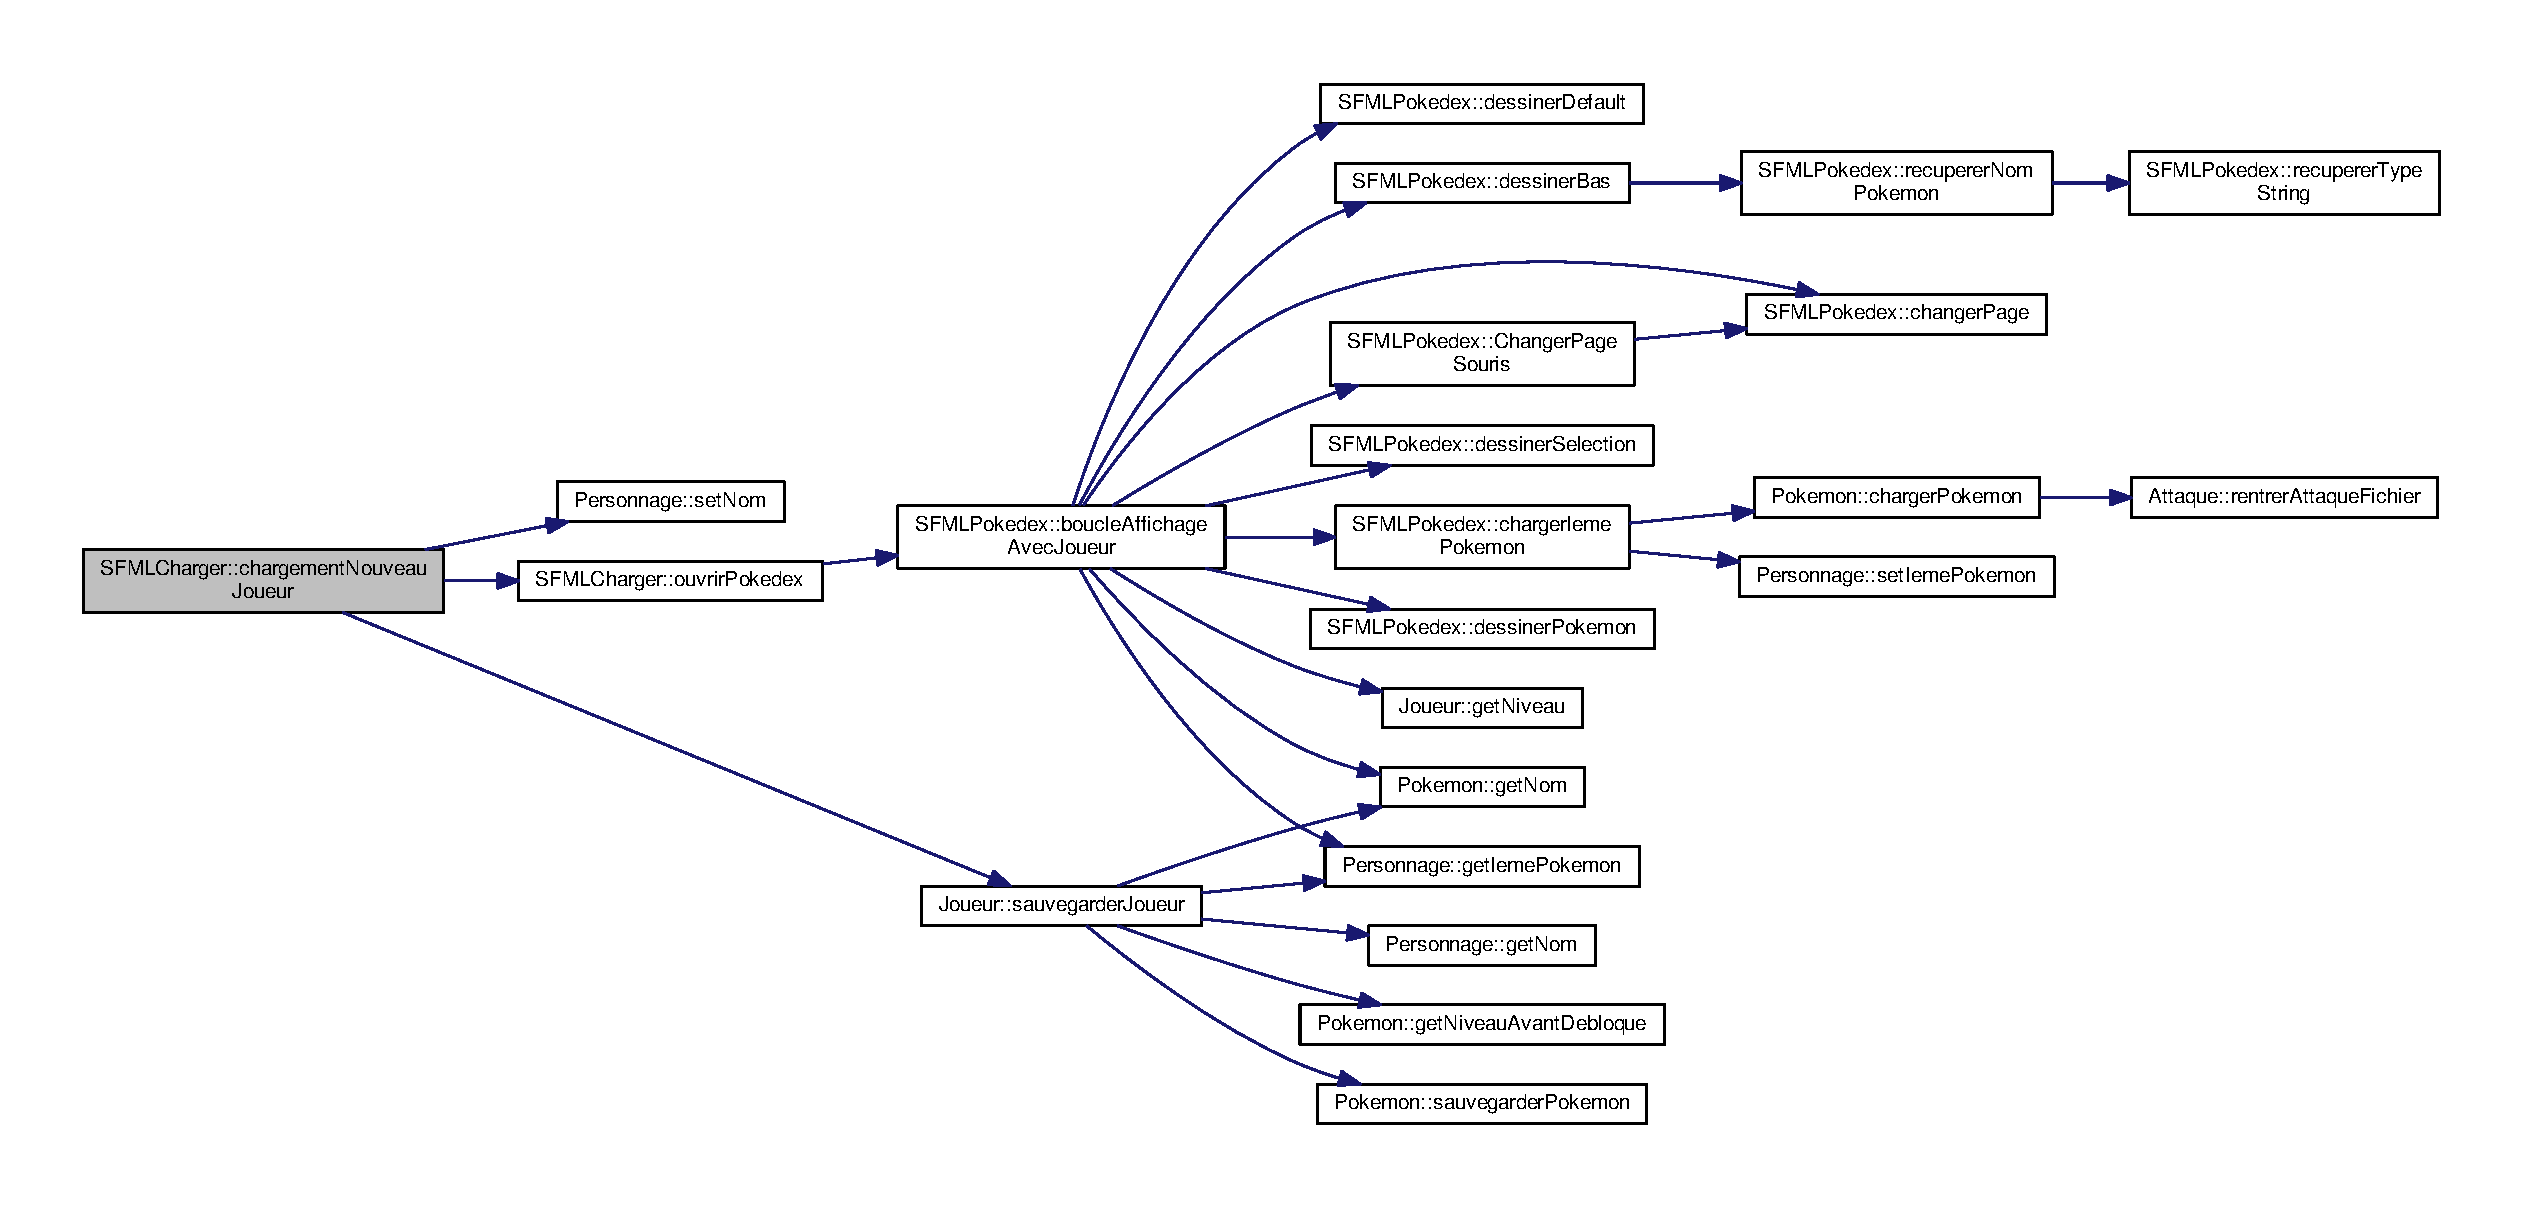
\includegraphics[width=350pt]{class_s_f_m_l_charger_a4c3135a3fa16c88f94cbef9c2ca2c2d8_cgraph}
\end{center}
\end{figure}
Voici le graphe des appelants de cette fonction \+:\nopagebreak
\begin{figure}[H]
\begin{center}
\leavevmode
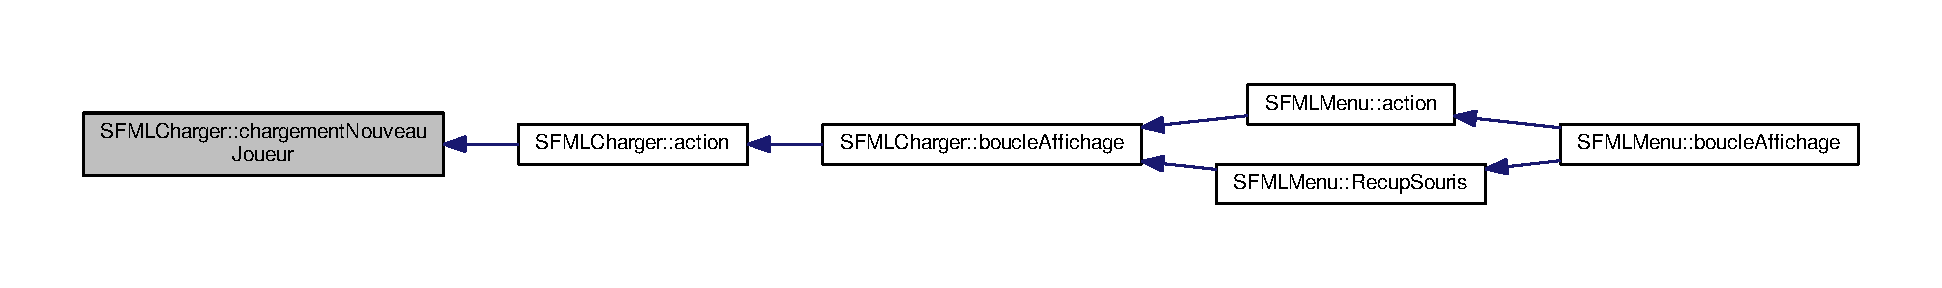
\includegraphics[width=350pt]{class_s_f_m_l_charger_a4c3135a3fa16c88f94cbef9c2ca2c2d8_icgraph}
\end{center}
\end{figure}
\mbox{\Hypertarget{class_s_f_m_l_charger_a988a052585ee0fe9e61535d5027a6f81}\label{class_s_f_m_l_charger_a988a052585ee0fe9e61535d5027a6f81}} 
\index{S\+F\+M\+L\+Charger@{S\+F\+M\+L\+Charger}!lancer\+Combat@{lancer\+Combat}}
\index{lancer\+Combat@{lancer\+Combat}!S\+F\+M\+L\+Charger@{S\+F\+M\+L\+Charger}}
\subsubsection{\texorpdfstring{lancer\+Combat()}{lancerCombat()}}
{\footnotesize\ttfamily void S\+F\+M\+L\+Charger\+::lancer\+Combat (\begin{DoxyParamCaption}\item[{\hyperlink{class_joueur}{Joueur} \&}]{joueur,  }\item[{\hyperlink{class_adversaire}{Adversaire} \&}]{adversaire }\end{DoxyParamCaption})\hspace{0.3cm}{\ttfamily [private]}}



S\textquotesingle{}occupe d\textquotesingle{}initialiser un nouveau joueur puis de le sauvegarder dans un fichier. 


\begin{DoxyParams}{Paramètres}
{\em } & \\
\hline
\end{DoxyParams}
Voici le graphe des appelants de cette fonction \+:\nopagebreak
\begin{figure}[H]
\begin{center}
\leavevmode
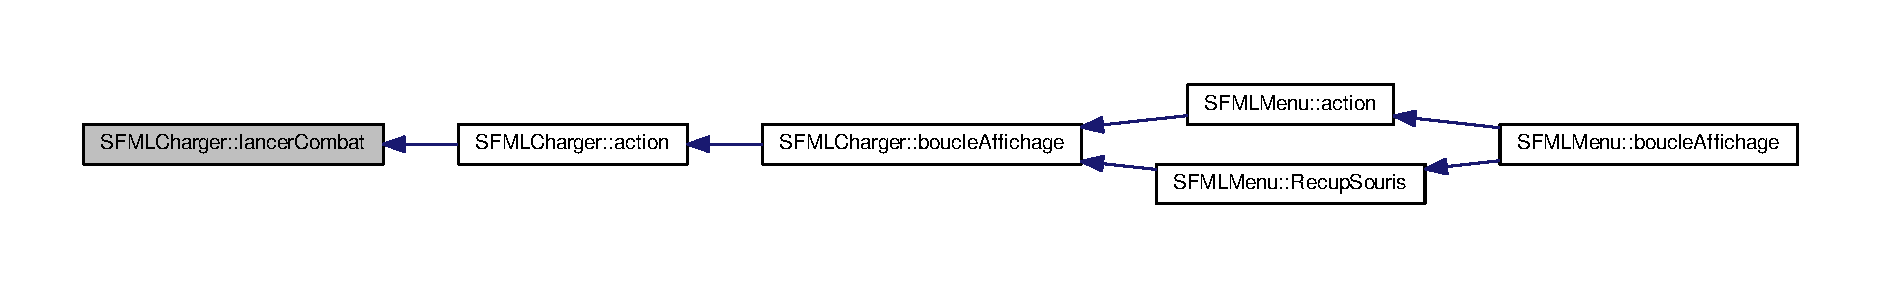
\includegraphics[width=350pt]{class_s_f_m_l_charger_a988a052585ee0fe9e61535d5027a6f81_icgraph}
\end{center}
\end{figure}
\mbox{\Hypertarget{class_s_f_m_l_charger_a67c610529df46560908104f963d741f1}\label{class_s_f_m_l_charger_a67c610529df46560908104f963d741f1}} 
\index{S\+F\+M\+L\+Charger@{S\+F\+M\+L\+Charger}!ouvrir\+Pokedex@{ouvrir\+Pokedex}}
\index{ouvrir\+Pokedex@{ouvrir\+Pokedex}!S\+F\+M\+L\+Charger@{S\+F\+M\+L\+Charger}}
\subsubsection{\texorpdfstring{ouvrir\+Pokedex()}{ouvrirPokedex()}}
{\footnotesize\ttfamily void S\+F\+M\+L\+Charger\+::ouvrir\+Pokedex (\begin{DoxyParamCaption}\item[{\hyperlink{class_joueur}{Joueur} \&}]{joueur }\end{DoxyParamCaption})\hspace{0.3cm}{\ttfamily [private]}}



S\textquotesingle{}occupe d\textquotesingle{}initialiser les pokémons du joueur. 


\begin{DoxyParams}{Paramètres}
{\em } & \\
\hline
\end{DoxyParams}
Voici le graphe d\textquotesingle{}appel pour cette fonction \+:\nopagebreak
\begin{figure}[H]
\begin{center}
\leavevmode
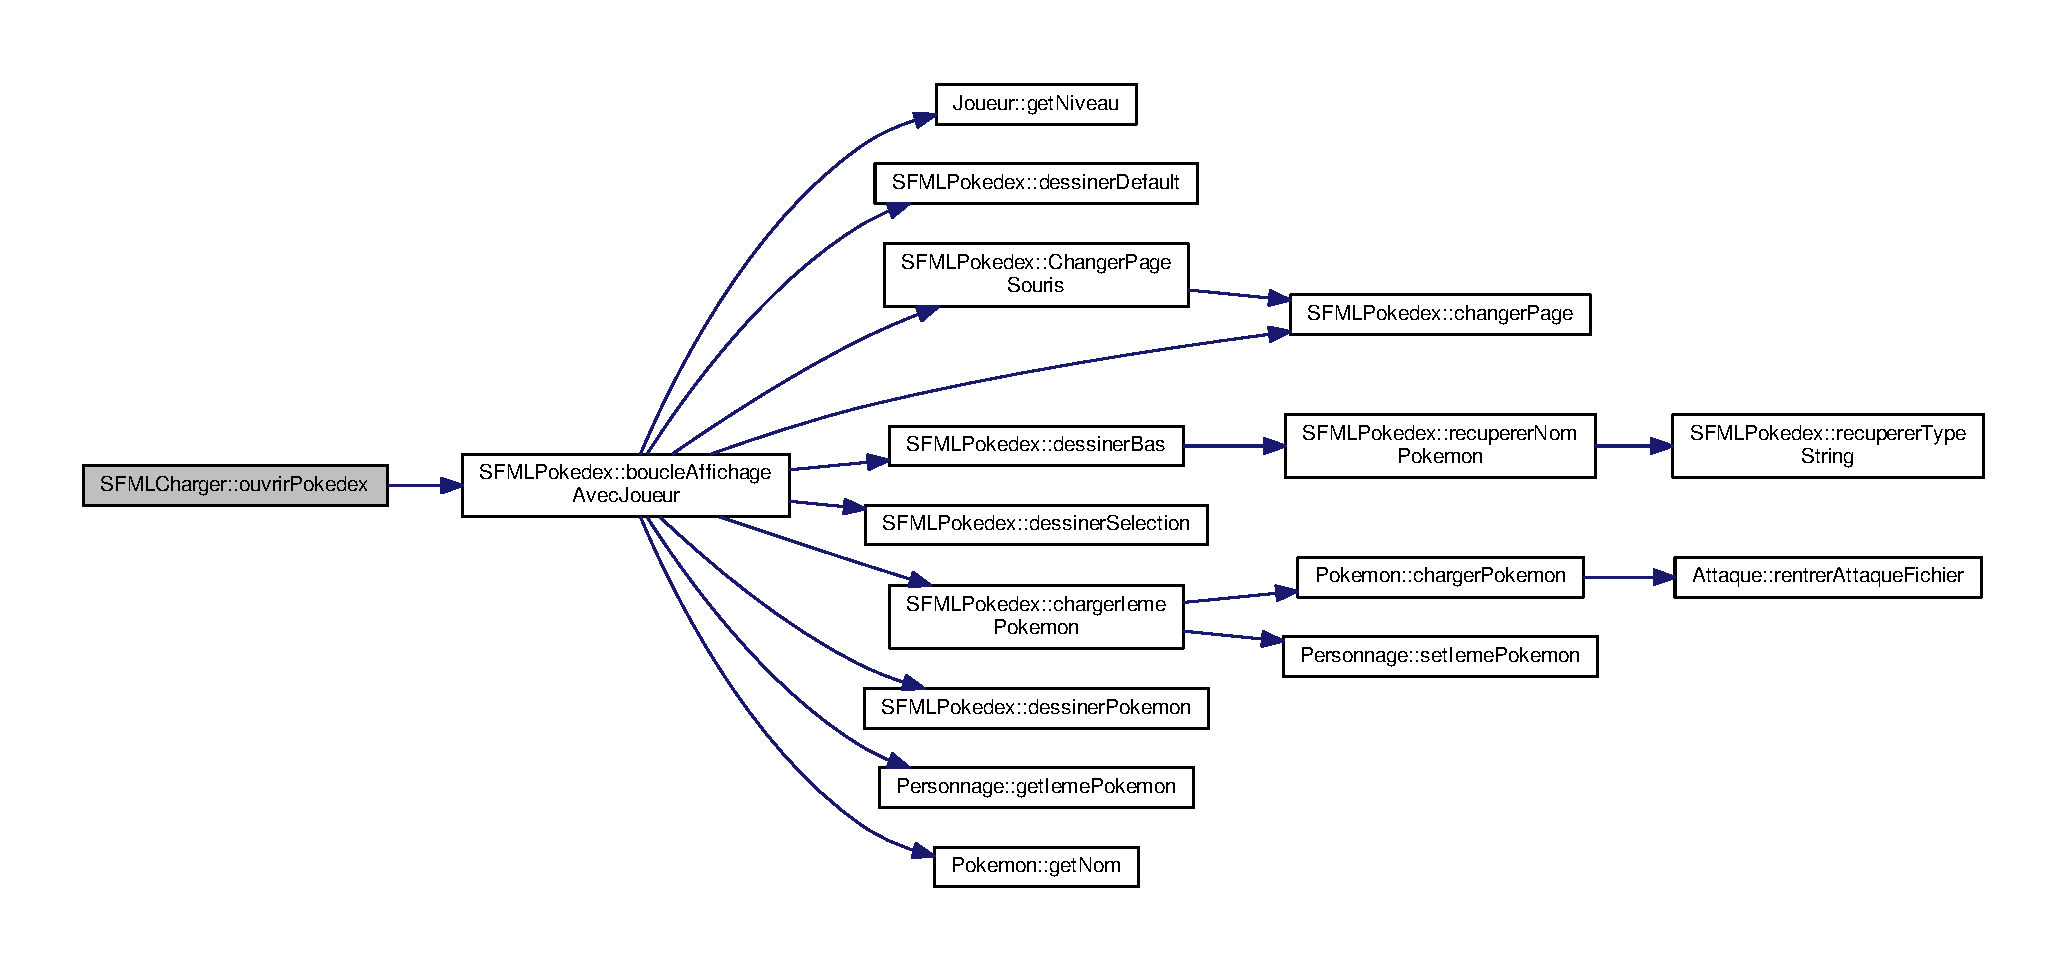
\includegraphics[width=350pt]{class_s_f_m_l_charger_a67c610529df46560908104f963d741f1_cgraph}
\end{center}
\end{figure}
Voici le graphe des appelants de cette fonction \+:\nopagebreak
\begin{figure}[H]
\begin{center}
\leavevmode
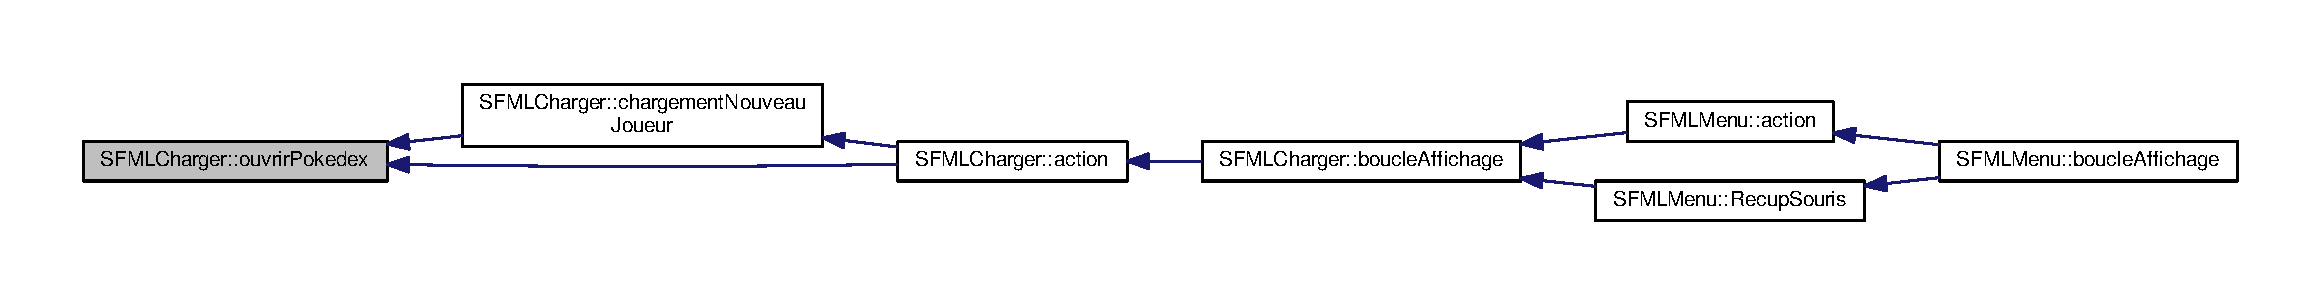
\includegraphics[width=350pt]{class_s_f_m_l_charger_a67c610529df46560908104f963d741f1_icgraph}
\end{center}
\end{figure}


La documentation de cette classe a été générée à partir des fichiers suivants \+:\begin{DoxyCompactItemize}
\item 
/home/corentin/\+Documents/lifap4/src/\+S\+F\+M\+L\+Charger/S\+F\+M\+L\+Charger.\+h\item 
/home/corentin/\+Documents/lifap4/src/\+S\+F\+M\+L\+Charger/\hyperlink{_s_f_m_l_charger_8cpp}{S\+F\+M\+L\+Charger.\+cpp}\end{DoxyCompactItemize}

\hypertarget{class_s_f_m_l_combat}{}\section{Référence de la classe S\+F\+M\+L\+Combat}
\label{class_s_f_m_l_combat}\index{S\+F\+M\+L\+Combat@{S\+F\+M\+L\+Combat}}


La classe gérant la partie I\+HM du combat.  




{\ttfamily \#include \char`\"{}src/\+S\+F\+M\+L\+Combat/\+S\+F\+M\+L.\+h\char`\"{}}



Graphe de collaboration de S\+F\+M\+L\+Combat\+:\nopagebreak
\begin{figure}[H]
\begin{center}
\leavevmode
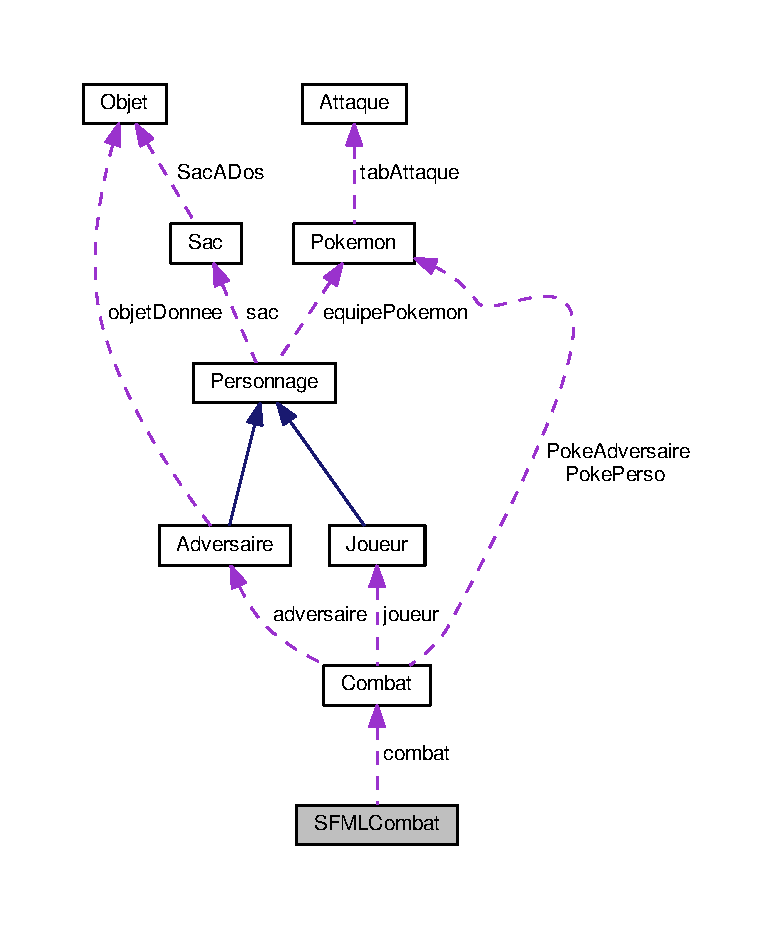
\includegraphics[width=350pt]{class_s_f_m_l_combat__coll__graph}
\end{center}
\end{figure}
\subsection*{Fonctions membres publiques}
\begin{DoxyCompactItemize}
\item 
\hyperlink{class_s_f_m_l_combat_a11ee4d8a8bc7f6cf85658af0f4b4b2a2}{S\+F\+M\+L\+Combat} (sf\+::\+Render\+Window \&menu\+Window, \hyperlink{class_combat}{Combat} \&combat\+En\+Cours)
\begin{DoxyCompactList}\small\item\em Constructeur de \hyperlink{class_s_f_m_l_combat}{S\+F\+M\+L\+Combat}. \end{DoxyCompactList}\item 
\hyperlink{class_s_f_m_l_combat_ac8e843e7ab09e8e8c18f9ddde4f17d6c}{S\+F\+M\+L\+Combat} (\hyperlink{class_combat}{Combat} \&combat\+En\+Cours)
\begin{DoxyCompactList}\small\item\em Constructeur de \hyperlink{class_s_f_m_l_combat}{S\+F\+M\+L\+Combat}. \end{DoxyCompactList}\item 
\hyperlink{class_s_f_m_l_combat_a28a895c7f9efdbe12cb47e3495500346}{S\+F\+M\+L\+Combat} (sf\+::\+Render\+Window \&menu\+Window)
\begin{DoxyCompactList}\small\item\em Constructeur de \hyperlink{class_s_f_m_l_combat}{S\+F\+M\+L\+Combat}. \end{DoxyCompactList}\item 
void \hyperlink{class_s_f_m_l_combat_a39155235e6275b4d63b9317b9561843e}{aff\+Boucle} ()
\begin{DoxyCompactList}\small\item\em La boucle principale de Jeu. \end{DoxyCompactList}\item 
void \hyperlink{class_s_f_m_l_combat_a116d70985530e3c46e5b60adc910a1fb}{aff\+Boucle\+IA} ()
\begin{DoxyCompactList}\small\item\em La boucle principale de Jeu (version combat IA) \end{DoxyCompactList}\end{DoxyCompactItemize}
\subsection*{Fonctions membres privées}
\begin{DoxyCompactItemize}
\item 
\hyperlink{class_combat}{Combat} $\ast$ \hyperlink{class_s_f_m_l_combat_a1529363beee93ae18694046822ea2e53}{get\+Combat\+Ref} ()
\begin{DoxyCompactList}\small\item\em Permet de récupérer un pointeur sur combat. \end{DoxyCompactList}\item 
bool \hyperlink{class_s_f_m_l_combat_af7ddb137c3bbaff70d2c566137c2cbb7}{test\+Pokemon\+En\+Vie} ()
\begin{DoxyCompactList}\small\item\em Test si une équipe \hyperlink{class_pokemon}{Pokemon} entière est KO. \end{DoxyCompactList}\item 
int \hyperlink{class_s_f_m_l_combat_a2665ce99eeccb4bdb1e032086a9feb04}{pokemon\+KO} ()
\begin{DoxyCompactList}\small\item\em Test si un des \hyperlink{class_pokemon}{Pokemon} combattant est KO. \end{DoxyCompactList}\item 
void \hyperlink{class_s_f_m_l_combat_ace8cd35d8b2bbc86478a7a28bf0996b4}{aff\+Gagnant} ()
\begin{DoxyCompactList}\small\item\em Boucle d\textquotesingle{}affichage de fin de partie. \end{DoxyCompactList}\item 
void \hyperlink{class_s_f_m_l_combat_aea2c9616512a2cb0c5e7e2f676a5daab}{dessiner\+Gagnant} ()
\begin{DoxyCompactList}\small\item\em Dessine l\textquotesingle{}écran de fin de partie. \end{DoxyCompactList}\item 
void \hyperlink{class_s_f_m_l_combat_a8803b5fb491ebcba31787b0aa20a9c07}{aff\+Attaque} ()
\begin{DoxyCompactList}\small\item\em Boucle d\textquotesingle{}affichage du menu attaque. \end{DoxyCompactList}\item 
void \hyperlink{class_s_f_m_l_combat_a55c6728be410efdf2ca919a9ee44728a}{aff\+Objet} ()
\begin{DoxyCompactList}\small\item\em Boucle d\textquotesingle{}affichage du menu objet. \end{DoxyCompactList}\item 
void \hyperlink{class_s_f_m_l_combat_a578125c9faee0eebfaa898b5d6ae6f6e}{dessiner\+Selection\+Objet} (int position\+Objet)
\begin{DoxyCompactList}\small\item\em Dessine le curseur de sélection. \end{DoxyCompactList}\item 
int \hyperlink{class_s_f_m_l_combat_a06e5c66f031d48316b7d779a9589c18e}{calcul\+Prochaine\+Position\+Objet} (sf\+::\+Event event, int position\+Objet)
\begin{DoxyCompactList}\small\item\em Calcul de la prochaine position objet. \end{DoxyCompactList}\item 
void \hyperlink{class_s_f_m_l_combat_ac41423229acd874f68463a462fdfce08}{se\+Deplacer\+Objet} (sf\+::\+Event event, int \&position\+Objet)
\begin{DoxyCompactList}\small\item\em Modifie position\+Objet. \end{DoxyCompactList}\item 
void \hyperlink{class_s_f_m_l_combat_a82520574af06d7d4bcb145f0a37fe691}{dessiner\+Objet} ()
\begin{DoxyCompactList}\small\item\em Dessine les sprites des objets. \end{DoxyCompactList}\item 
void \hyperlink{class_s_f_m_l_combat_ab8d4dfb3e7e4ca9722e52c1ef5fa897d}{aff\+Changer\+Pokemon} ()
\begin{DoxyCompactList}\small\item\em Boucle d\textquotesingle{}affichage du menu Changer de \hyperlink{class_pokemon}{Pokemon}. \end{DoxyCompactList}\item 
void \hyperlink{class_s_f_m_l_combat_ab37fca053d9f0e3529502c69f0de1055}{dessiner\+Selection\+Pokemon} (int position\+Pokemon)
\begin{DoxyCompactList}\small\item\em Dessine le curseur de sélection. \end{DoxyCompactList}\item 
int \hyperlink{class_s_f_m_l_combat_ab0728cc1b2fcc52112165ec8e3e14eb6}{calcul\+Prochaine\+Position\+Pokemon} (sf\+::\+Event event, int position\+Pokemon)
\begin{DoxyCompactList}\small\item\em Calcul de la prochaine position \hyperlink{class_pokemon}{Pokemon}. \end{DoxyCompactList}\item 
void \hyperlink{class_s_f_m_l_combat_ad6e349e747401615a1c3d5c56e59be76}{se\+Deplacer\+Pokemon} (sf\+::\+Event event, int \&position\+Pokemon)
\begin{DoxyCompactList}\small\item\em Modifie position\+Pokemon. \end{DoxyCompactList}\item 
void \hyperlink{class_s_f_m_l_combat_a22523f39138086a3b118a896ca214c4d}{dessiner\+Pokemon} ()
\begin{DoxyCompactList}\small\item\em Dessine les sprites des \hyperlink{class_pokemon}{Pokemon}. \end{DoxyCompactList}\item 
void \hyperlink{class_s_f_m_l_combat_a4b2bed6ea12c96a58e55d968b1652597}{aff\+Combat} (int \&Choix\+Menu1, int \&Choix\+Bis1, int \&Choix\+Menu2, int \&Choix\+Bis2)
\begin{DoxyCompactList}\small\item\em Boucle d\textquotesingle{}affichage des actions. \end{DoxyCompactList}\item 
void \hyperlink{class_s_f_m_l_combat_acc968da97d4c933f516e67b0356e3d73}{afficher\+Action} ()
\begin{DoxyCompactList}\small\item\em Affichage textuel des actions effectués. \end{DoxyCompactList}\item 
void \hyperlink{class_s_f_m_l_combat_af3dbb1374820d004fdf5907397760335}{calcul\+Priorite} (int Choix\+Menu1, int Choix\+Bis1, int Choix\+Menu2, int Choix\+Bis2)
\begin{DoxyCompactList}\small\item\em Calcul de la priorité des Joueurs. \end{DoxyCompactList}\item 
void \hyperlink{class_s_f_m_l_combat_a9d307eb8a3289a694486f30b56ca402d}{init\+Main\+Window} ()
\item 
void \hyperlink{class_s_f_m_l_combat_a5d363c2d06e7f0505990bf12866d0595}{init\+Fight\+Window} ()
\item 
void \hyperlink{class_s_f_m_l_combat_aba0eacdc425cc859b8533060ead79564}{init\+Menu\+Window} ()
\item 
void \hyperlink{class_s_f_m_l_combat_ab5de8e3048e2549352cea43a3ff636d4}{aff\+Pokemon} ()
\item 
void \hyperlink{class_s_f_m_l_combat_ae641a09e3a5a8e50b3fe8352207e4748}{aff\+Tour} ()
\item 
void \hyperlink{class_s_f_m_l_combat_ad5ab6d579c0da644135ae1e51e44f890}{aff\+Barre\+De\+Vie} ()
\item 
void \hyperlink{class_s_f_m_l_combat_a557bb97c785650b8d28ff913ca86081a}{ecrire\+Menu} ()
\item 
void \hyperlink{class_s_f_m_l_combat_a83899ae7d061225976857060d2a16388}{ecrire\+Attaque} ()
\item 
void \hyperlink{class_s_f_m_l_combat_a9a9295e8e7f369f0443ee5618004f0d9}{selection\+Menu} ()
\item 
int \hyperlink{class_s_f_m_l_combat_ab856672c59db95d55c7c28cd3a1eee93}{changer\+Menu} ()
\item 
void \hyperlink{class_s_f_m_l_combat_a796b43eec3296bc9d66e2618069f5abe}{se\+Deplacer} (sf\+::\+Event event)
\item 
int \hyperlink{class_s_f_m_l_combat_a2e7feee45aae418d7545cc71534e6148}{calcul\+Prochaine\+Position} (sf\+::\+Event event)
\item 
bool \hyperlink{class_s_f_m_l_combat_a97bf8a2d3300663aacbb8899bbbf3472}{test\+Pokemon\+En\+Vie\+IA} ()
\begin{DoxyCompactList}\small\item\em Test si un des \hyperlink{class_pokemon}{Pokemon} combattant est KO (version combat contre IA) \end{DoxyCompactList}\item 
void \hyperlink{class_s_f_m_l_combat_ad72f480db9eb3f134e3736b1acb228c8}{choix\+Menu} (int \&Choix\+Menu2, int \&Choix\+Bis2)
\begin{DoxyCompactList}\small\item\em Reflexion de l\textquotesingle{}IA sur l\textquotesingle{}action à effectuer. \end{DoxyCompactList}\item 
bool \hyperlink{class_s_f_m_l_combat_ac8720bfe637fdaa932ef45240493bbd6}{chance\+Attaquer} ()
\begin{DoxyCompactList}\small\item\em Chance d\textquotesingle{}attaquer. \end{DoxyCompactList}\item 
bool \hyperlink{class_s_f_m_l_combat_a00370ff45d848befb5d35c52bd1db2d5}{chance\+Objet} ()
\begin{DoxyCompactList}\small\item\em Chance d\textquotesingle{}utiliser un objet. \end{DoxyCompactList}\item 
bool \hyperlink{class_s_f_m_l_combat_a4ba9a6e1f0c91eb425ac83649e443375}{chance\+Pokemon} ()
\begin{DoxyCompactList}\small\item\em Chance de changer de \hyperlink{class_pokemon}{Pokemon}. \end{DoxyCompactList}\item 
int \hyperlink{class_s_f_m_l_combat_ab1f7a0fa82f0cfd9c0a0e1c321f5f7e7}{choix\+Attaque} ()
\begin{DoxyCompactList}\small\item\em Choix de l\textquotesingle{}attaque à lancer. \end{DoxyCompactList}\item 
int \hyperlink{class_s_f_m_l_combat_aa22c1c2665846e97e2eef331af8420d1}{choix\+Objet} ()
\begin{DoxyCompactList}\small\item\em Choix de l\textquotesingle{}objet à utiliser. \end{DoxyCompactList}\item 
int \hyperlink{class_s_f_m_l_combat_a4d5b43087452661e39479026a886d1b6}{choix\+Pokemon} ()
\begin{DoxyCompactList}\small\item\em Choix du \hyperlink{class_pokemon}{Pokemon} à faire rentrer sur le terrain. \end{DoxyCompactList}\item 
float \hyperlink{class_s_f_m_l_combat_a226dd0d639049753aef1fef95cf9a3f0}{Avantage\+Type} (const \hyperlink{class_pokemon}{Pokemon} \&Pkmn\+IA, const \hyperlink{_attaque_8h_a1d1cfd8ffb84e947f82999c682b666a7}{Type} \&type\+Joueur)
\begin{DoxyCompactList}\small\item\em Calcul l\textquotesingle{}avantage d\textquotesingle{}un type par rapport aux types d\textquotesingle{}un \hyperlink{class_pokemon}{Pokemon}. \end{DoxyCompactList}\end{DoxyCompactItemize}
\subsection*{Attributs privés}
\begin{DoxyCompactItemize}
\item 
sf\+::\+Render\+Window $\ast$ \hyperlink{class_s_f_m_l_combat_a78da4b3f5a924922d26db0b756531505}{main\+Window}
\begin{DoxyCompactList}\small\item\em Un pointeur sur la fenêtre de Jeu. \end{DoxyCompactList}\item 
sf\+::\+Rectangle\+Shape \hyperlink{class_s_f_m_l_combat_a3dbd6e3e3626b934d91feeecfdc75f2f}{boite\+Attaquer}
\begin{DoxyCompactList}\small\item\em Le rectangle définissant la boite \char`\"{}\+Attaquer\char`\"{}. \end{DoxyCompactList}\item 
sf\+::\+Rectangle\+Shape \hyperlink{class_s_f_m_l_combat_a7a7d3634ff67cf57c61d343e07800586}{boite\+Objet}
\begin{DoxyCompactList}\small\item\em Le rectangle définissant la boite \char`\"{}\+Utiliser objet\char`\"{}. \end{DoxyCompactList}\item 
sf\+::\+Rectangle\+Shape \hyperlink{class_s_f_m_l_combat_a752cb4de138e2aa37f12c237efea253e}{boite\+Pokemon}
\begin{DoxyCompactList}\small\item\em Le rectangle définissant la boite \char`\"{}\+Changer de Pokemon\char`\"{}. \end{DoxyCompactList}\item 
sf\+::\+Rectangle\+Shape \hyperlink{class_s_f_m_l_combat_a0a9270612142eaa1406152265ba839b2}{boite\+Fuir}
\begin{DoxyCompactList}\small\item\em Le rectangle définissant la boite \char`\"{}\+Fuir\char`\"{}. \end{DoxyCompactList}\item 
sf\+::\+Rectangle\+Shape \hyperlink{class_s_f_m_l_combat_aced33a85a7133efb947d8c472f770ec1}{pkmn\+J1}
\begin{DoxyCompactList}\small\item\em Le rectangle définissant le \hyperlink{class_pokemon}{Pokemon} du J1. \end{DoxyCompactList}\item 
sf\+::\+Rectangle\+Shape \hyperlink{class_s_f_m_l_combat_ac85b298cc8a29f2ea61b5d1e76a4f427}{pkmn\+J2}
\begin{DoxyCompactList}\small\item\em Le rectangle définissant la \hyperlink{class_pokemon}{Pokemon} du J2. \end{DoxyCompactList}\item 
sf\+::\+Font \hyperlink{class_s_f_m_l_combat_a38592e5f22439c81e07f3ffee4012a5f}{font}
\begin{DoxyCompactList}\small\item\em La police d\textquotesingle{}écriture utilisé pour l\textquotesingle{}affichage de texte. \end{DoxyCompactList}\item 
unsigned int \hyperlink{class_s_f_m_l_combat_aad9f3c91f2ec93a927d14d21d18df8bf}{dimX}
\begin{DoxyCompactList}\small\item\em La largeur de la fenêtre de Jeu. \end{DoxyCompactList}\item 
unsigned int \hyperlink{class_s_f_m_l_combat_a07171a9f601831e2ffba2cab5c072bba}{dimY}
\begin{DoxyCompactList}\small\item\em La hauteur de la fenêtre de Jeu. \end{DoxyCompactList}\item 
int \hyperlink{class_s_f_m_l_combat_a21d930da921cc2aa1cdc55b417c2fe0b}{position}
\begin{DoxyCompactList}\small\item\em La position du curseur dans les menus. \end{DoxyCompactList}\item 
\hyperlink{class_combat}{Combat} $\ast$ \hyperlink{class_s_f_m_l_combat_a3bddd4f06e74010cb91565b6b23a2f22}{combat}
\begin{DoxyCompactList}\small\item\em Le combat étant actuellement géré par le module. \end{DoxyCompactList}\item 
int $\ast$ \hyperlink{class_s_f_m_l_combat_ac89c3f6d77a8238bf105586f861f1195}{Choix\+Menu}
\begin{DoxyCompactList}\small\item\em Le pointeur sur le choix de Menu. \end{DoxyCompactList}\item 
int $\ast$ \hyperlink{class_s_f_m_l_combat_ad76ea7634796fda2075edda681735375}{Choix\+Bis}
\begin{DoxyCompactList}\small\item\em Le pointeur sur le choix de Bis. \end{DoxyCompactList}\end{DoxyCompactItemize}


\subsection{Description détaillée}
La classe gérant la partie I\+HM du combat. 

Le module S\+F\+ML consiste en la gestion de l\textquotesingle{}affichage du combat ainsi que la communication Homme-\/\+Machine nécéssaire durant le combat.. 

\subsection{Documentation des constructeurs et destructeur}
\mbox{\Hypertarget{class_s_f_m_l_combat_a11ee4d8a8bc7f6cf85658af0f4b4b2a2}\label{class_s_f_m_l_combat_a11ee4d8a8bc7f6cf85658af0f4b4b2a2}} 
\index{S\+F\+M\+L\+Combat@{S\+F\+M\+L\+Combat}!S\+F\+M\+L\+Combat@{S\+F\+M\+L\+Combat}}
\index{S\+F\+M\+L\+Combat@{S\+F\+M\+L\+Combat}!S\+F\+M\+L\+Combat@{S\+F\+M\+L\+Combat}}
\subsubsection{\texorpdfstring{S\+F\+M\+L\+Combat()}{SFMLCombat()}\hspace{0.1cm}{\footnotesize\ttfamily [1/3]}}
{\footnotesize\ttfamily S\+F\+M\+L\+Combat\+::\+S\+F\+M\+L\+Combat (\begin{DoxyParamCaption}\item[{sf\+::\+Render\+Window \&}]{menu\+Window,  }\item[{\hyperlink{class_combat}{Combat} \&}]{combat\+En\+Cours }\end{DoxyParamCaption})}



Constructeur de \hyperlink{class_s_f_m_l_combat}{S\+F\+M\+L\+Combat}. 

Construit un objet de type \hyperlink{class_s_f_m_l_combat}{S\+F\+M\+L\+Combat} en utilisant une fenêtre déjà ouvertes et un combat déjà crée 
\begin{DoxyParams}[1]{Paramètres}
\mbox{\tt out}  & {\em menu\+Window} & correspond à la fenêtre que \hyperlink{class_s_f_m_l_combat}{S\+F\+M\+L\+Combat} utilisera comme fenêtre de jeu. \\
\hline
\mbox{\tt out}  & {\em combat\+En\+Cours} & correspond au combat que \hyperlink{class_s_f_m_l_combat}{S\+F\+M\+L\+Combat} doit gérér pour le jeu \\
\hline
\end{DoxyParams}
\mbox{\Hypertarget{class_s_f_m_l_combat_ac8e843e7ab09e8e8c18f9ddde4f17d6c}\label{class_s_f_m_l_combat_ac8e843e7ab09e8e8c18f9ddde4f17d6c}} 
\index{S\+F\+M\+L\+Combat@{S\+F\+M\+L\+Combat}!S\+F\+M\+L\+Combat@{S\+F\+M\+L\+Combat}}
\index{S\+F\+M\+L\+Combat@{S\+F\+M\+L\+Combat}!S\+F\+M\+L\+Combat@{S\+F\+M\+L\+Combat}}
\subsubsection{\texorpdfstring{S\+F\+M\+L\+Combat()}{SFMLCombat()}\hspace{0.1cm}{\footnotesize\ttfamily [2/3]}}
{\footnotesize\ttfamily S\+F\+M\+L\+Combat\+::\+S\+F\+M\+L\+Combat (\begin{DoxyParamCaption}\item[{\hyperlink{class_combat}{Combat} \&}]{combat\+En\+Cours }\end{DoxyParamCaption})}



Constructeur de \hyperlink{class_s_f_m_l_combat}{S\+F\+M\+L\+Combat}. 

Construit un objet de type \hyperlink{class_s_f_m_l_combat}{S\+F\+M\+L\+Combat} en utilisant un combat déjà crée 
\begin{DoxyParams}[1]{Paramètres}
\mbox{\tt out}  & {\em combat\+En\+Cours} & correspond au combat que \hyperlink{class_s_f_m_l_combat}{S\+F\+M\+L\+Combat} doit gérér pour le jeu \\
\hline
\end{DoxyParams}
\mbox{\Hypertarget{class_s_f_m_l_combat_a28a895c7f9efdbe12cb47e3495500346}\label{class_s_f_m_l_combat_a28a895c7f9efdbe12cb47e3495500346}} 
\index{S\+F\+M\+L\+Combat@{S\+F\+M\+L\+Combat}!S\+F\+M\+L\+Combat@{S\+F\+M\+L\+Combat}}
\index{S\+F\+M\+L\+Combat@{S\+F\+M\+L\+Combat}!S\+F\+M\+L\+Combat@{S\+F\+M\+L\+Combat}}
\subsubsection{\texorpdfstring{S\+F\+M\+L\+Combat()}{SFMLCombat()}\hspace{0.1cm}{\footnotesize\ttfamily [3/3]}}
{\footnotesize\ttfamily S\+F\+M\+L\+Combat\+::\+S\+F\+M\+L\+Combat (\begin{DoxyParamCaption}\item[{sf\+::\+Render\+Window \&}]{menu\+Window }\end{DoxyParamCaption})}



Constructeur de \hyperlink{class_s_f_m_l_combat}{S\+F\+M\+L\+Combat}. 

Construit un objet de type \hyperlink{class_s_f_m_l_combat}{S\+F\+M\+L\+Combat} en utilisant une fenêtre déjà ouvertes 
\begin{DoxyParams}[1]{Paramètres}
\mbox{\tt out}  & {\em menu\+Window} & correspond à la fenêtre que \hyperlink{class_s_f_m_l_combat}{S\+F\+M\+L\+Combat} utilisera comme fenêtre de jeu. \\
\hline
\end{DoxyParams}


\subsection{Documentation des fonctions membres}
\mbox{\Hypertarget{class_s_f_m_l_combat_a8803b5fb491ebcba31787b0aa20a9c07}\label{class_s_f_m_l_combat_a8803b5fb491ebcba31787b0aa20a9c07}} 
\index{S\+F\+M\+L\+Combat@{S\+F\+M\+L\+Combat}!aff\+Attaque@{aff\+Attaque}}
\index{aff\+Attaque@{aff\+Attaque}!S\+F\+M\+L\+Combat@{S\+F\+M\+L\+Combat}}
\subsubsection{\texorpdfstring{aff\+Attaque()}{affAttaque()}}
{\footnotesize\ttfamily void S\+F\+M\+L\+Combat\+::aff\+Attaque (\begin{DoxyParamCaption}{ }\end{DoxyParamCaption})\hspace{0.3cm}{\ttfamily [private]}}



Boucle d\textquotesingle{}affichage du menu attaque. 

Permet de gérer le menu d\textquotesingle{}attaque, et de gérer la selection d\textquotesingle{}une attaque Voici le graphe d\textquotesingle{}appel pour cette fonction \+:\nopagebreak
\begin{figure}[H]
\begin{center}
\leavevmode
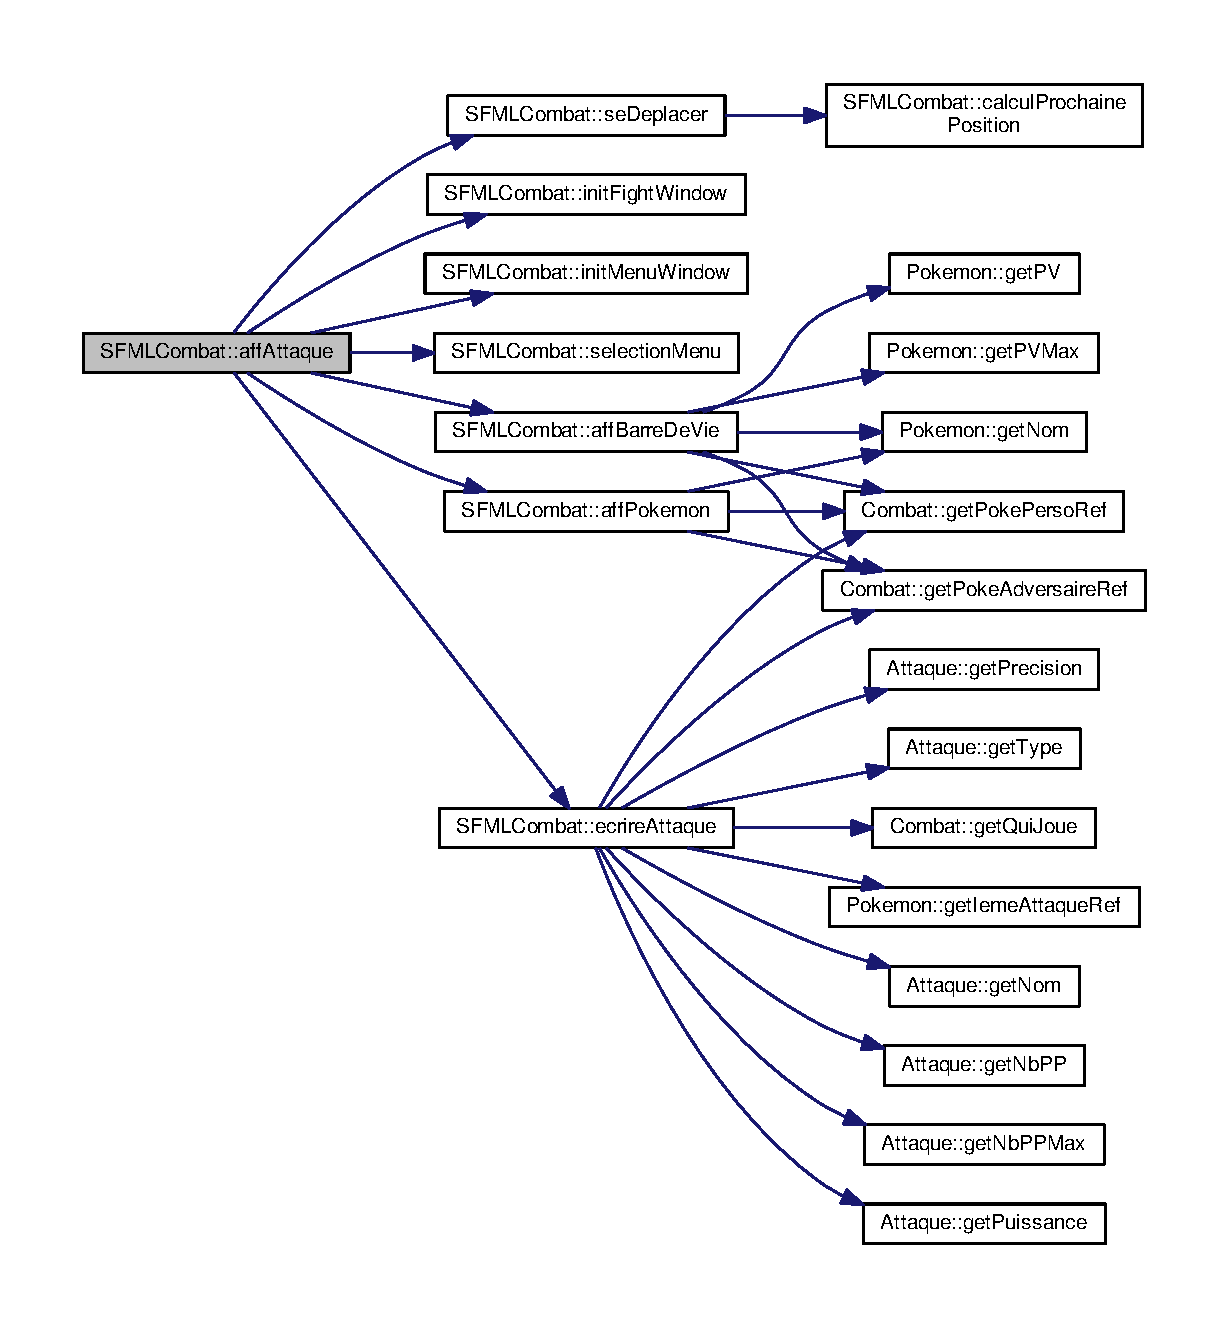
\includegraphics[width=350pt]{class_s_f_m_l_combat_a8803b5fb491ebcba31787b0aa20a9c07_cgraph}
\end{center}
\end{figure}
Voici le graphe des appelants de cette fonction \+:\nopagebreak
\begin{figure}[H]
\begin{center}
\leavevmode
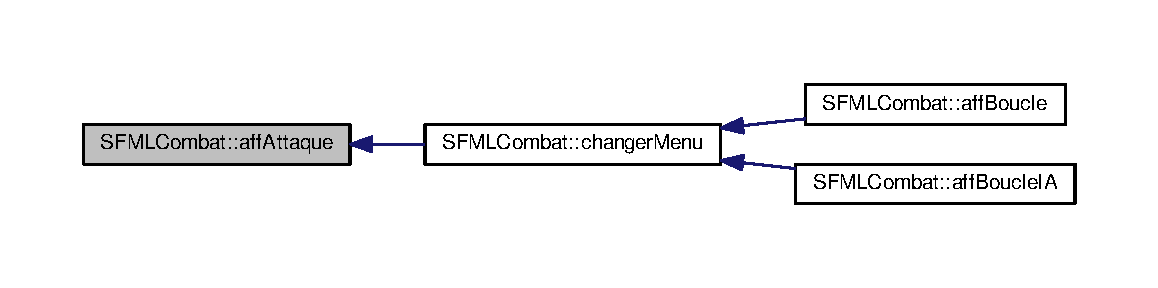
\includegraphics[width=350pt]{class_s_f_m_l_combat_a8803b5fb491ebcba31787b0aa20a9c07_icgraph}
\end{center}
\end{figure}
\mbox{\Hypertarget{class_s_f_m_l_combat_ad5ab6d579c0da644135ae1e51e44f890}\label{class_s_f_m_l_combat_ad5ab6d579c0da644135ae1e51e44f890}} 
\index{S\+F\+M\+L\+Combat@{S\+F\+M\+L\+Combat}!aff\+Barre\+De\+Vie@{aff\+Barre\+De\+Vie}}
\index{aff\+Barre\+De\+Vie@{aff\+Barre\+De\+Vie}!S\+F\+M\+L\+Combat@{S\+F\+M\+L\+Combat}}
\subsubsection{\texorpdfstring{aff\+Barre\+De\+Vie()}{affBarreDeVie()}}
{\footnotesize\ttfamily void S\+F\+M\+L\+Combat\+::aff\+Barre\+De\+Vie (\begin{DoxyParamCaption}{ }\end{DoxyParamCaption})\hspace{0.3cm}{\ttfamily [private]}}

$\vert$brief Affichage de la barre de vie

Dessine la barre de vie pour chaque \hyperlink{class_pokemon}{Pokemon} étant en combat, et gére l\textquotesingle{}évolution de la vie au cours du combat Voici le graphe d\textquotesingle{}appel pour cette fonction \+:\nopagebreak
\begin{figure}[H]
\begin{center}
\leavevmode
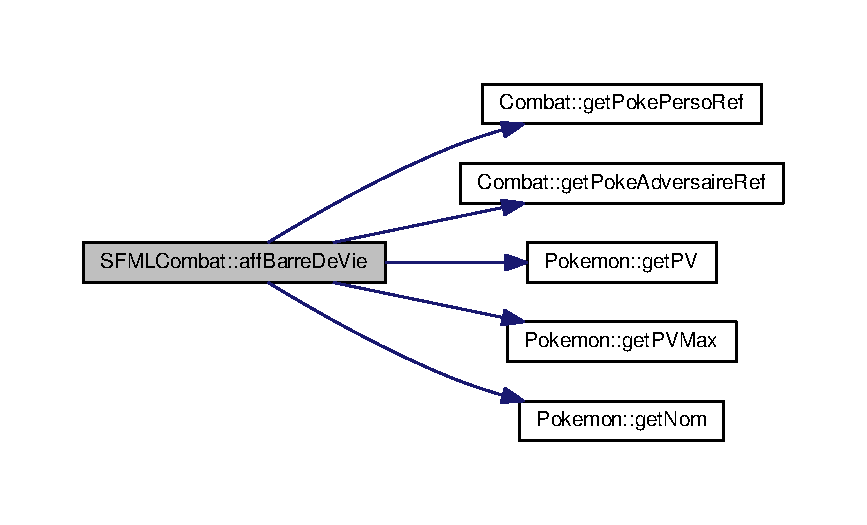
\includegraphics[width=350pt]{class_s_f_m_l_combat_ad5ab6d579c0da644135ae1e51e44f890_cgraph}
\end{center}
\end{figure}
Voici le graphe des appelants de cette fonction \+:\nopagebreak
\begin{figure}[H]
\begin{center}
\leavevmode
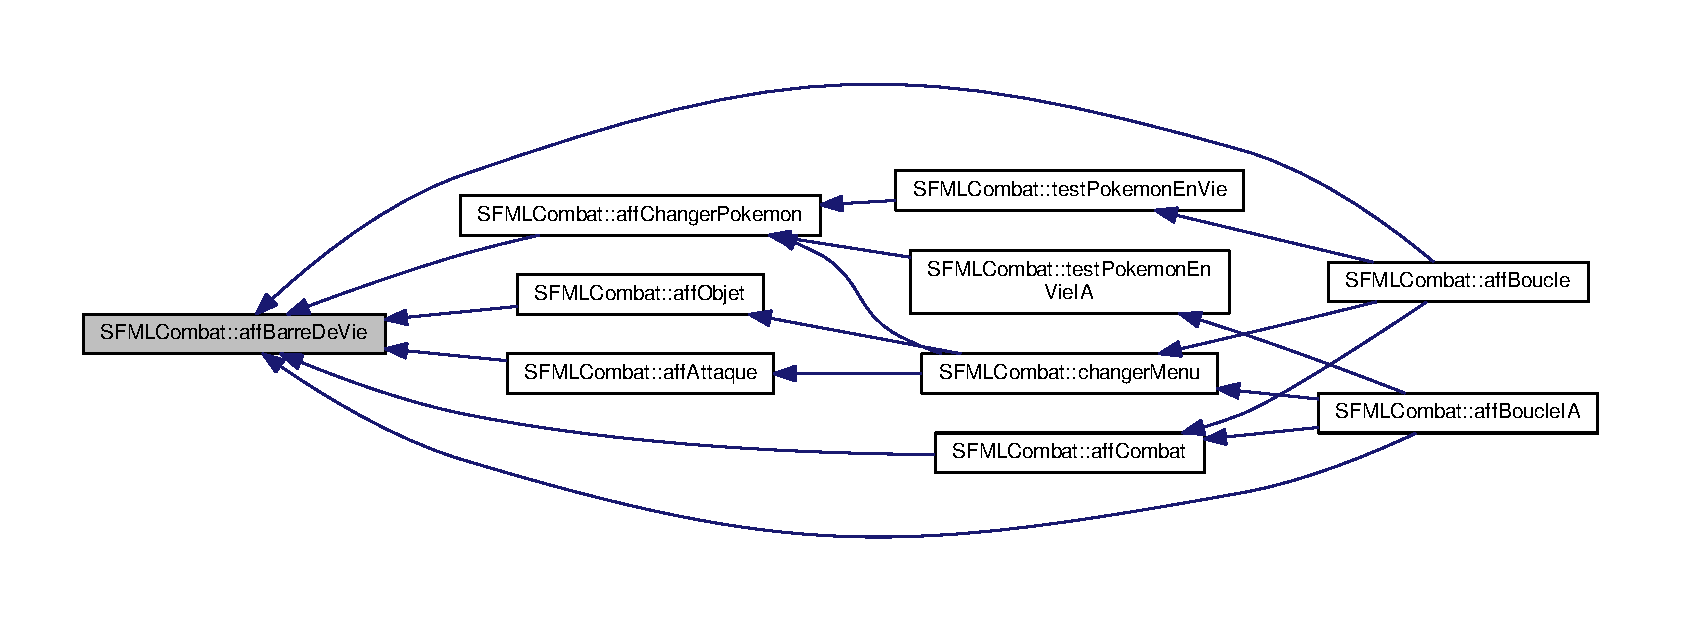
\includegraphics[width=350pt]{class_s_f_m_l_combat_ad5ab6d579c0da644135ae1e51e44f890_icgraph}
\end{center}
\end{figure}
\mbox{\Hypertarget{class_s_f_m_l_combat_a39155235e6275b4d63b9317b9561843e}\label{class_s_f_m_l_combat_a39155235e6275b4d63b9317b9561843e}} 
\index{S\+F\+M\+L\+Combat@{S\+F\+M\+L\+Combat}!aff\+Boucle@{aff\+Boucle}}
\index{aff\+Boucle@{aff\+Boucle}!S\+F\+M\+L\+Combat@{S\+F\+M\+L\+Combat}}
\subsubsection{\texorpdfstring{aff\+Boucle()}{affBoucle()}}
{\footnotesize\ttfamily void S\+F\+M\+L\+Combat\+::aff\+Boucle (\begin{DoxyParamCaption}{ }\end{DoxyParamCaption})}



La boucle principale de Jeu. 

aff\+Boucle permet de démarrer le jeu et encapsulera toutes les autres boucles nécéssaire à l\textquotesingle{}affichage du combat Voici le graphe d\textquotesingle{}appel pour cette fonction \+:\nopagebreak
\begin{figure}[H]
\begin{center}
\leavevmode
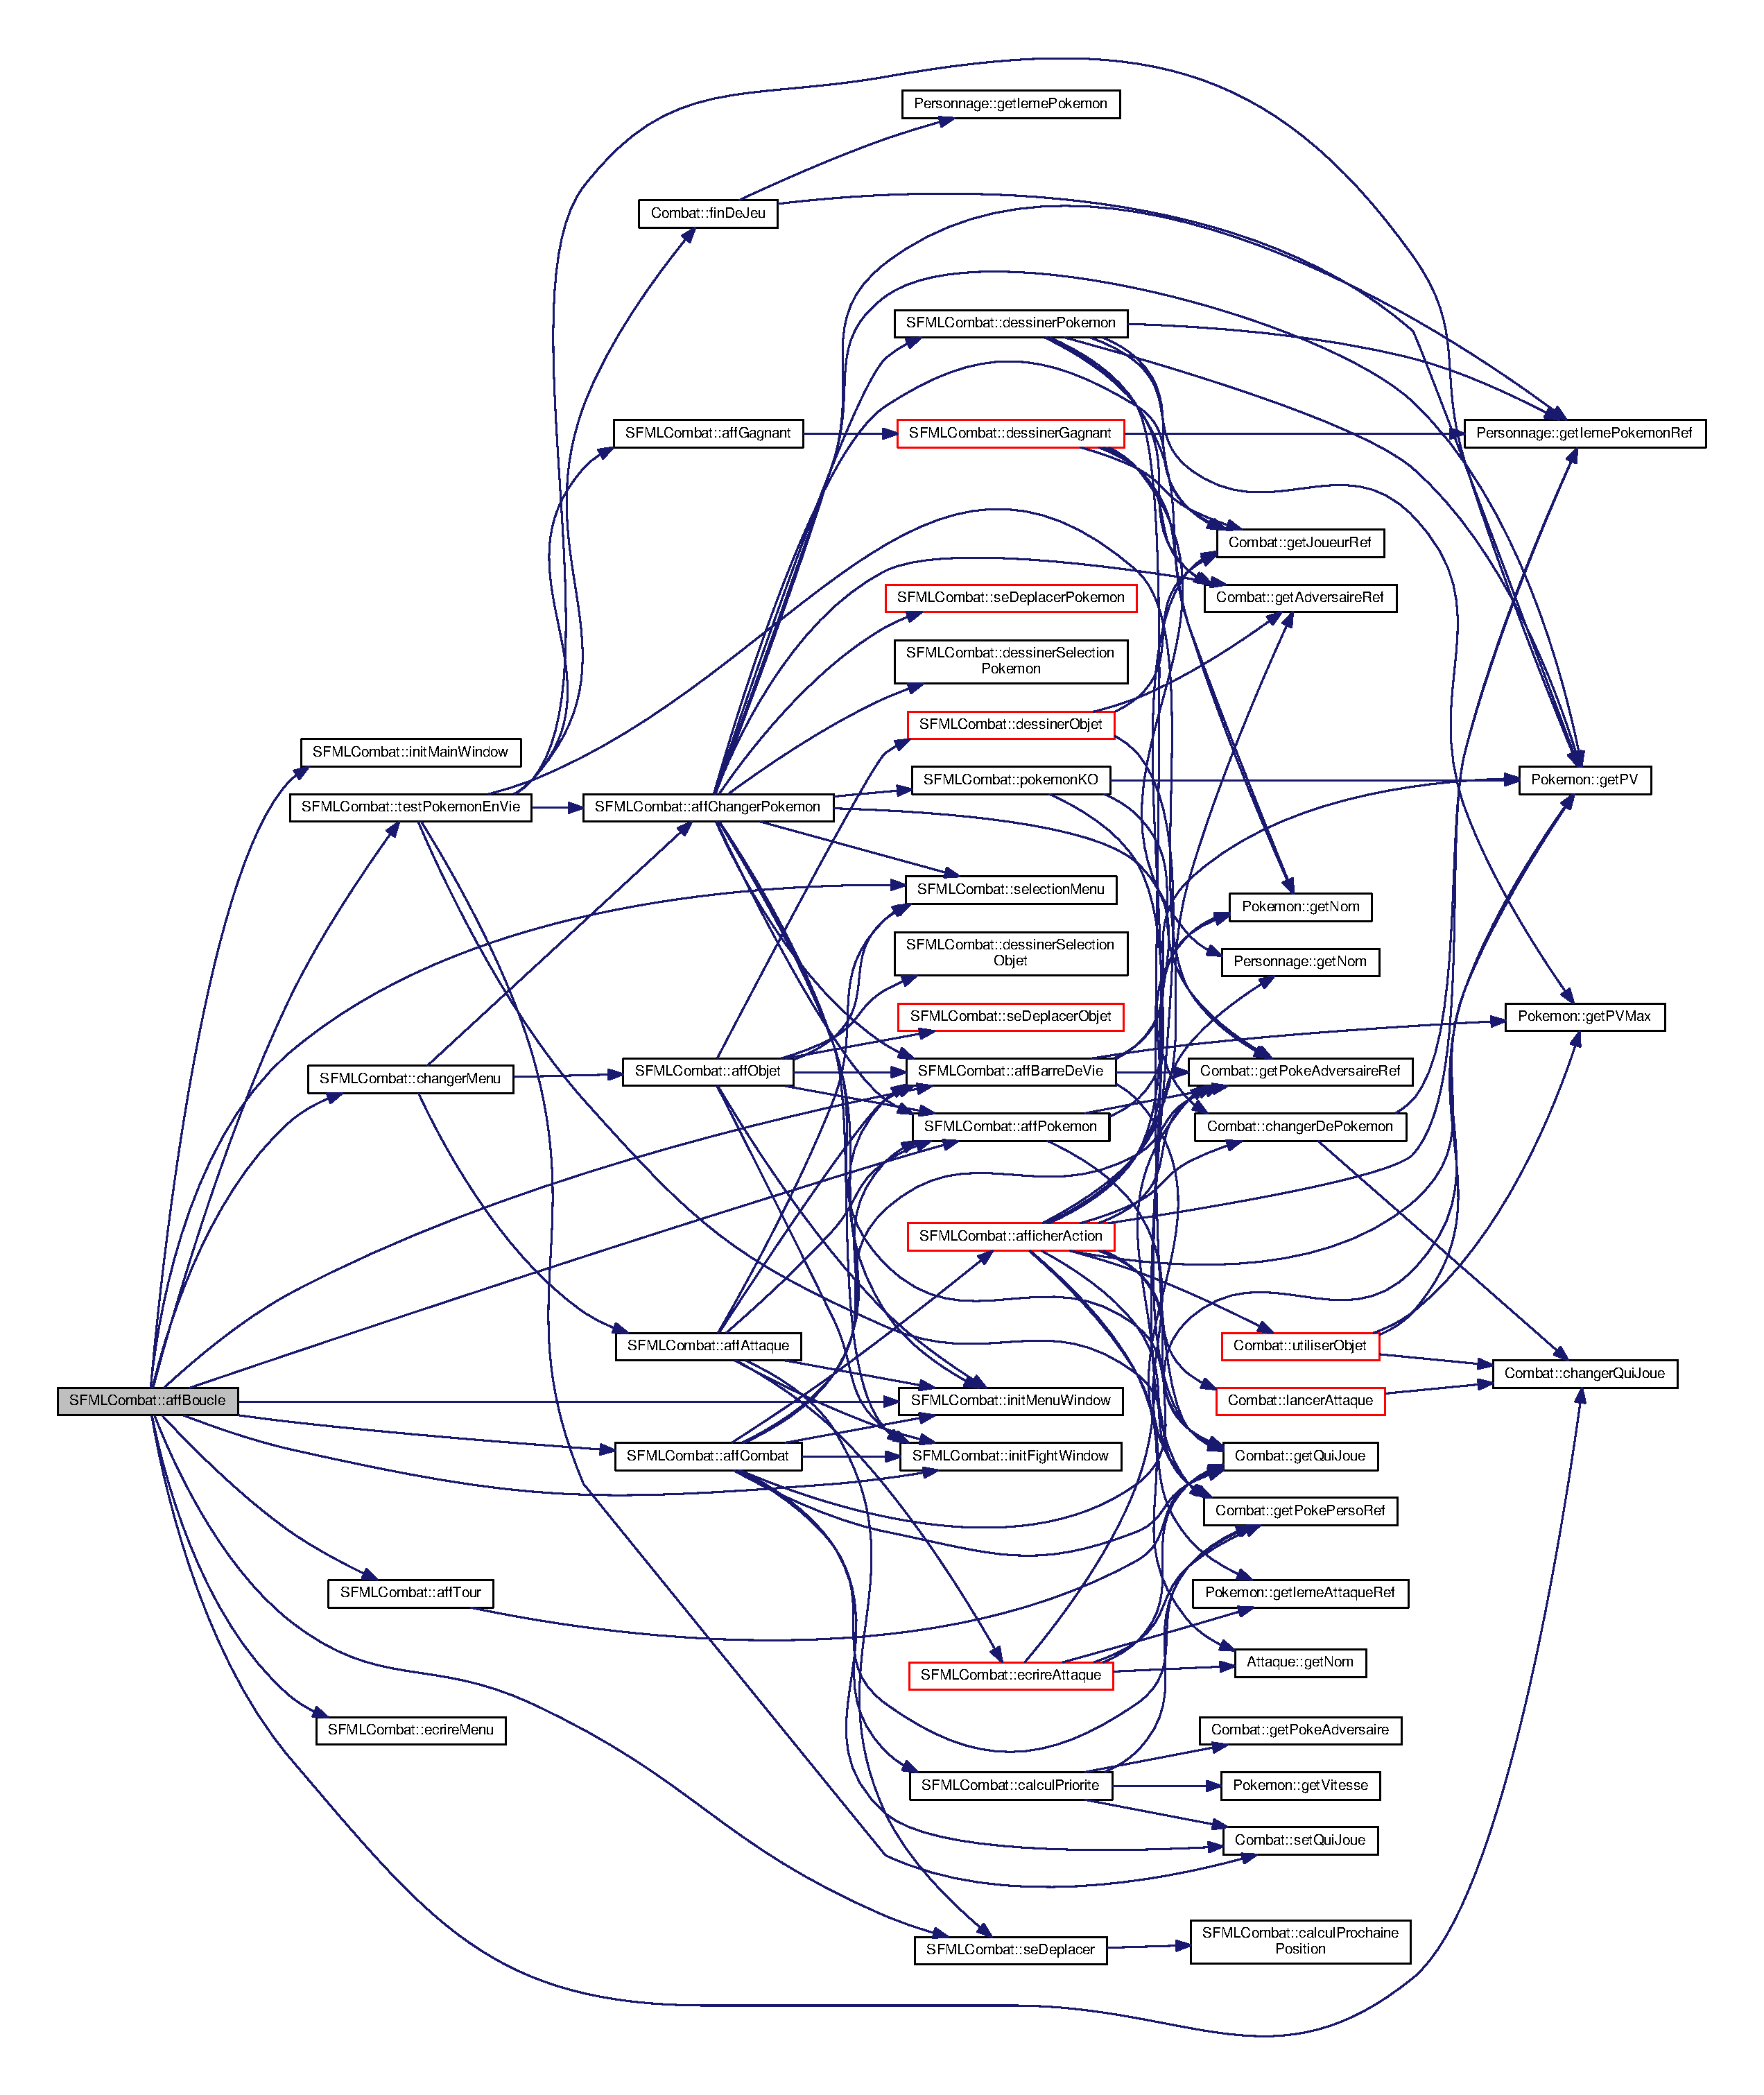
\includegraphics[width=350pt]{class_s_f_m_l_combat_a39155235e6275b4d63b9317b9561843e_cgraph}
\end{center}
\end{figure}
\mbox{\Hypertarget{class_s_f_m_l_combat_a116d70985530e3c46e5b60adc910a1fb}\label{class_s_f_m_l_combat_a116d70985530e3c46e5b60adc910a1fb}} 
\index{S\+F\+M\+L\+Combat@{S\+F\+M\+L\+Combat}!aff\+Boucle\+IA@{aff\+Boucle\+IA}}
\index{aff\+Boucle\+IA@{aff\+Boucle\+IA}!S\+F\+M\+L\+Combat@{S\+F\+M\+L\+Combat}}
\subsubsection{\texorpdfstring{aff\+Boucle\+I\+A()}{affBoucleIA()}}
{\footnotesize\ttfamily void S\+F\+M\+L\+Combat\+::aff\+Boucle\+IA (\begin{DoxyParamCaption}{ }\end{DoxyParamCaption})}



La boucle principale de Jeu (version combat IA) 

aff\+Boucle\+IA permet de démarrer le jeu et encapsulera toutes les autres boucles nécéssaire à l\textquotesingle{}affichage du combat (version combat IA) Voici le graphe d\textquotesingle{}appel pour cette fonction \+:\nopagebreak
\begin{figure}[H]
\begin{center}
\leavevmode
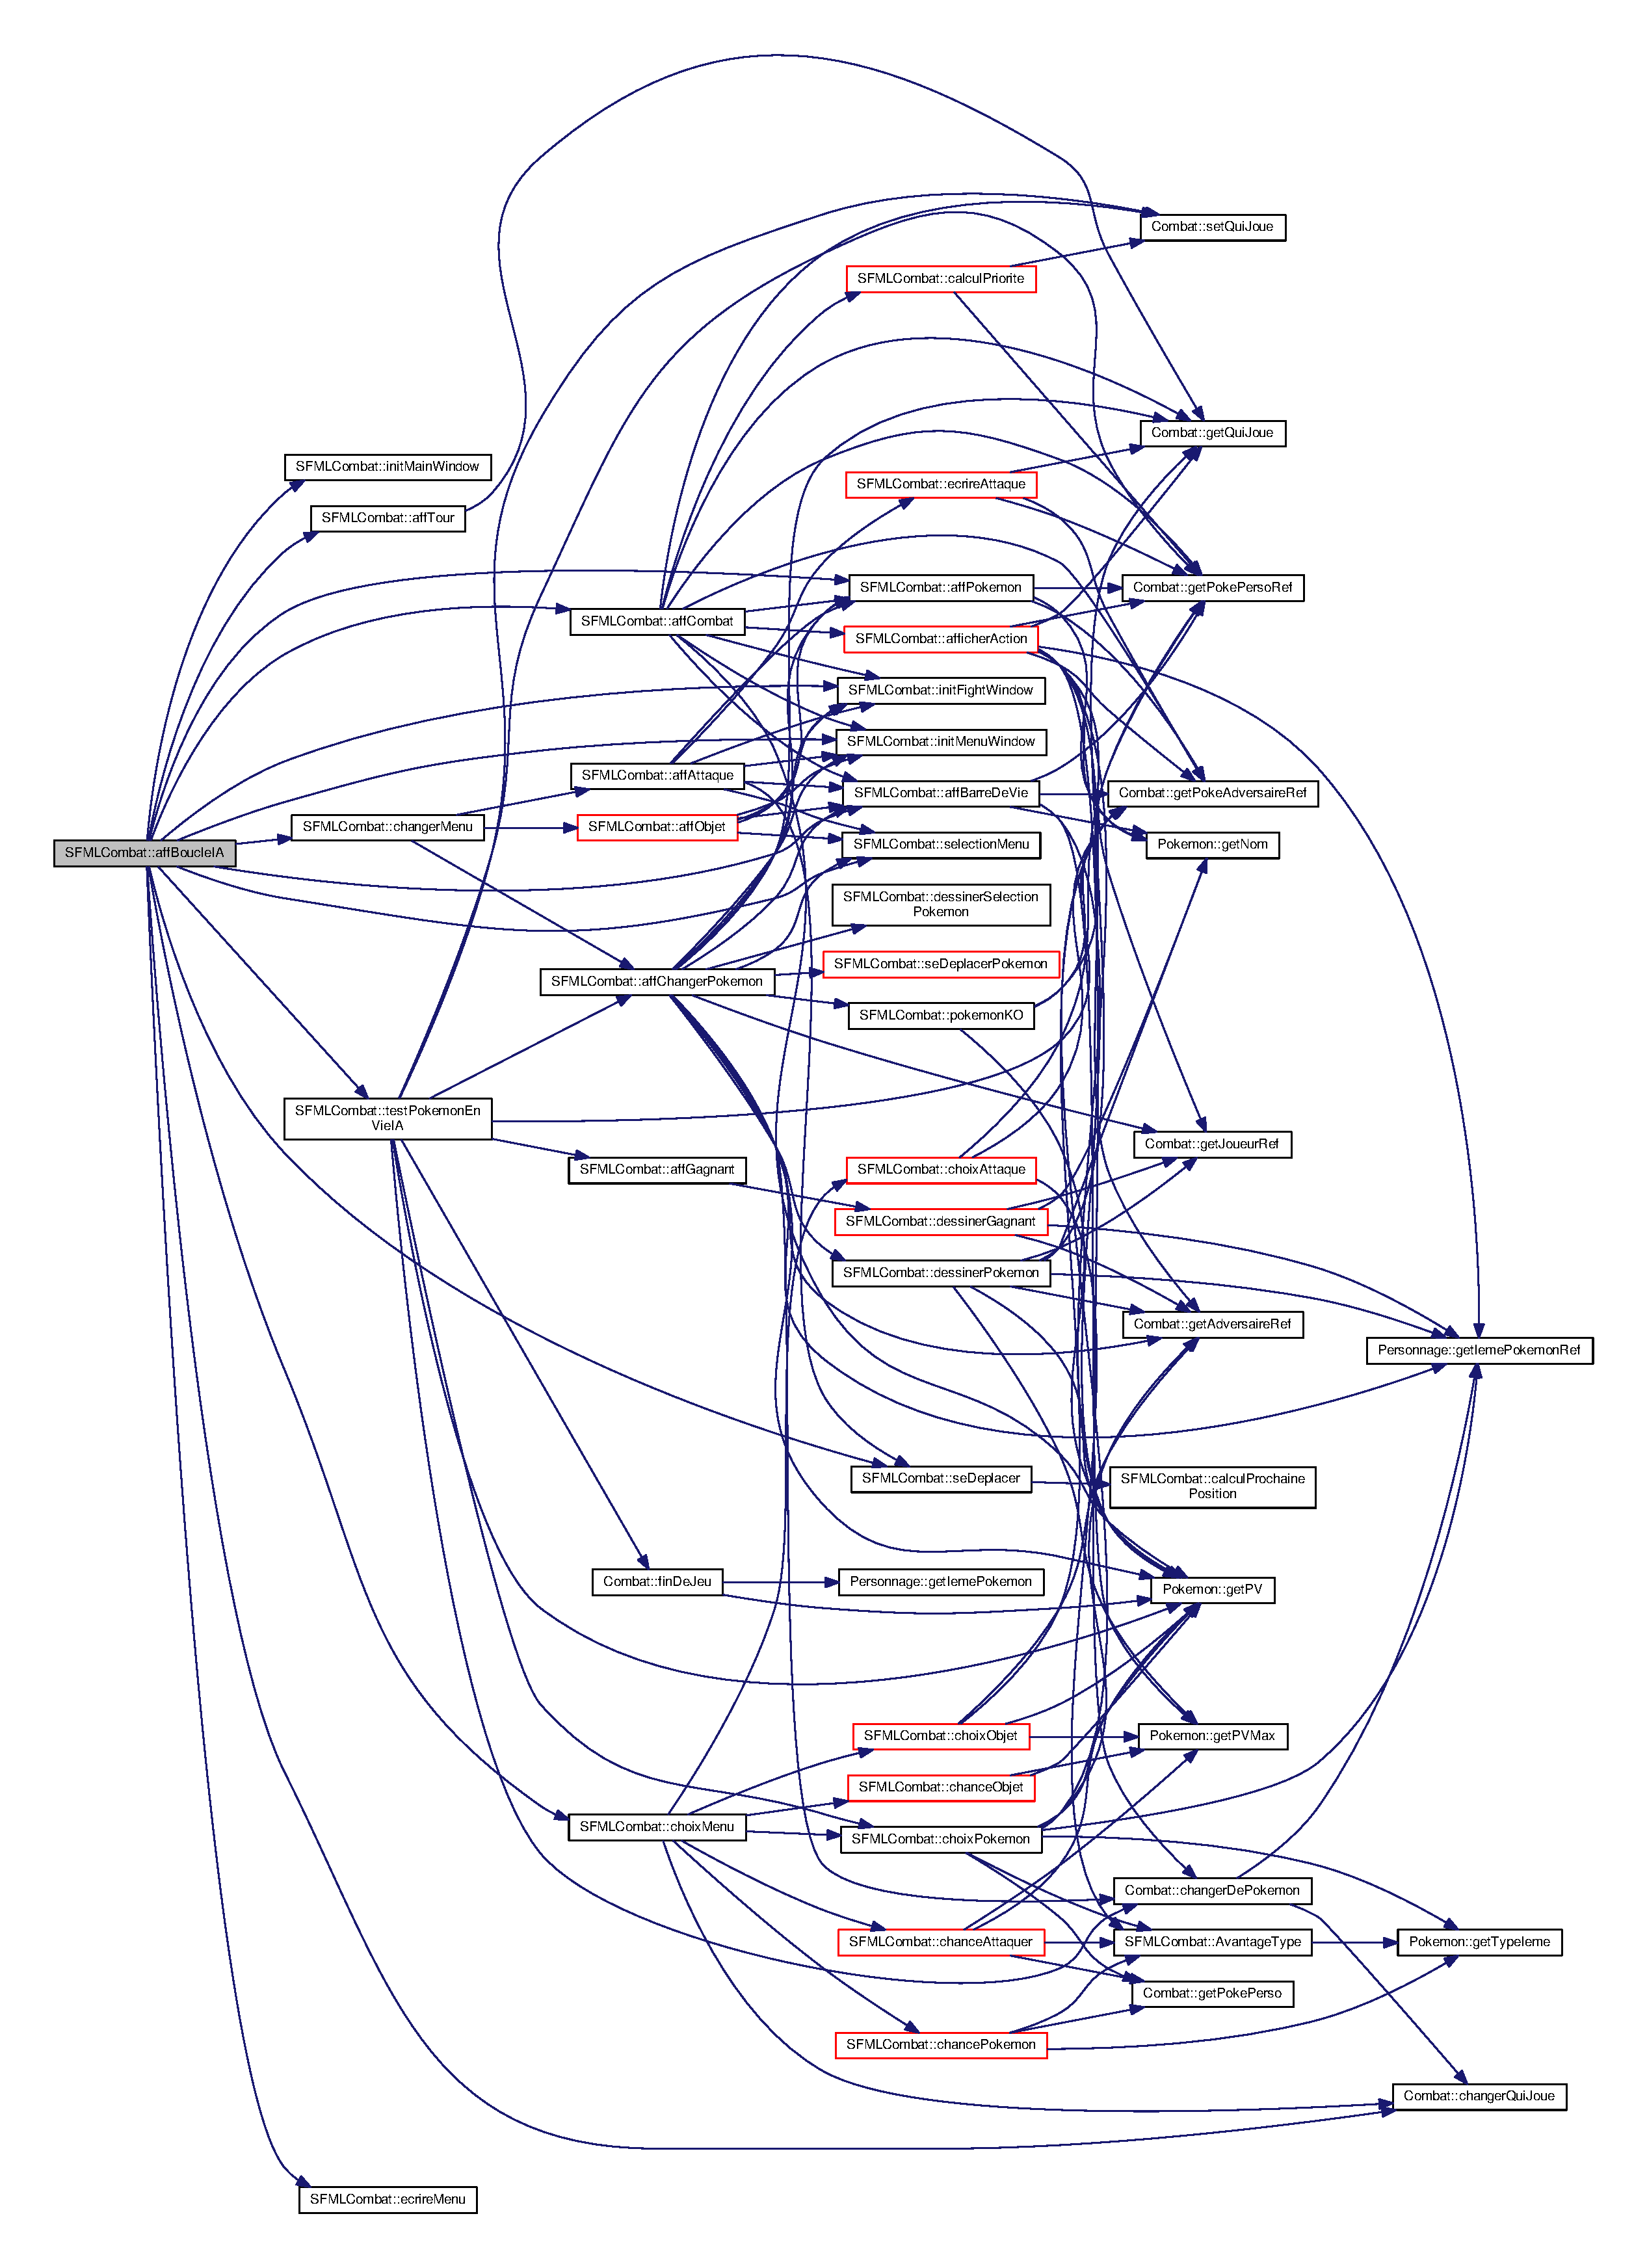
\includegraphics[width=350pt]{class_s_f_m_l_combat_a116d70985530e3c46e5b60adc910a1fb_cgraph}
\end{center}
\end{figure}
\mbox{\Hypertarget{class_s_f_m_l_combat_ab8d4dfb3e7e4ca9722e52c1ef5fa897d}\label{class_s_f_m_l_combat_ab8d4dfb3e7e4ca9722e52c1ef5fa897d}} 
\index{S\+F\+M\+L\+Combat@{S\+F\+M\+L\+Combat}!aff\+Changer\+Pokemon@{aff\+Changer\+Pokemon}}
\index{aff\+Changer\+Pokemon@{aff\+Changer\+Pokemon}!S\+F\+M\+L\+Combat@{S\+F\+M\+L\+Combat}}
\subsubsection{\texorpdfstring{aff\+Changer\+Pokemon()}{affChangerPokemon()}}
{\footnotesize\ttfamily void S\+F\+M\+L\+Combat\+::aff\+Changer\+Pokemon (\begin{DoxyParamCaption}{ }\end{DoxyParamCaption})\hspace{0.3cm}{\ttfamily [private]}}



Boucle d\textquotesingle{}affichage du menu Changer de \hyperlink{class_pokemon}{Pokemon}. 

Permet de gérer le menu \hyperlink{class_pokemon}{Pokemon}, et de gérer la selection d\textquotesingle{}un \hyperlink{class_pokemon}{Pokemon} pour le changement Voici le graphe d\textquotesingle{}appel pour cette fonction \+:\nopagebreak
\begin{figure}[H]
\begin{center}
\leavevmode
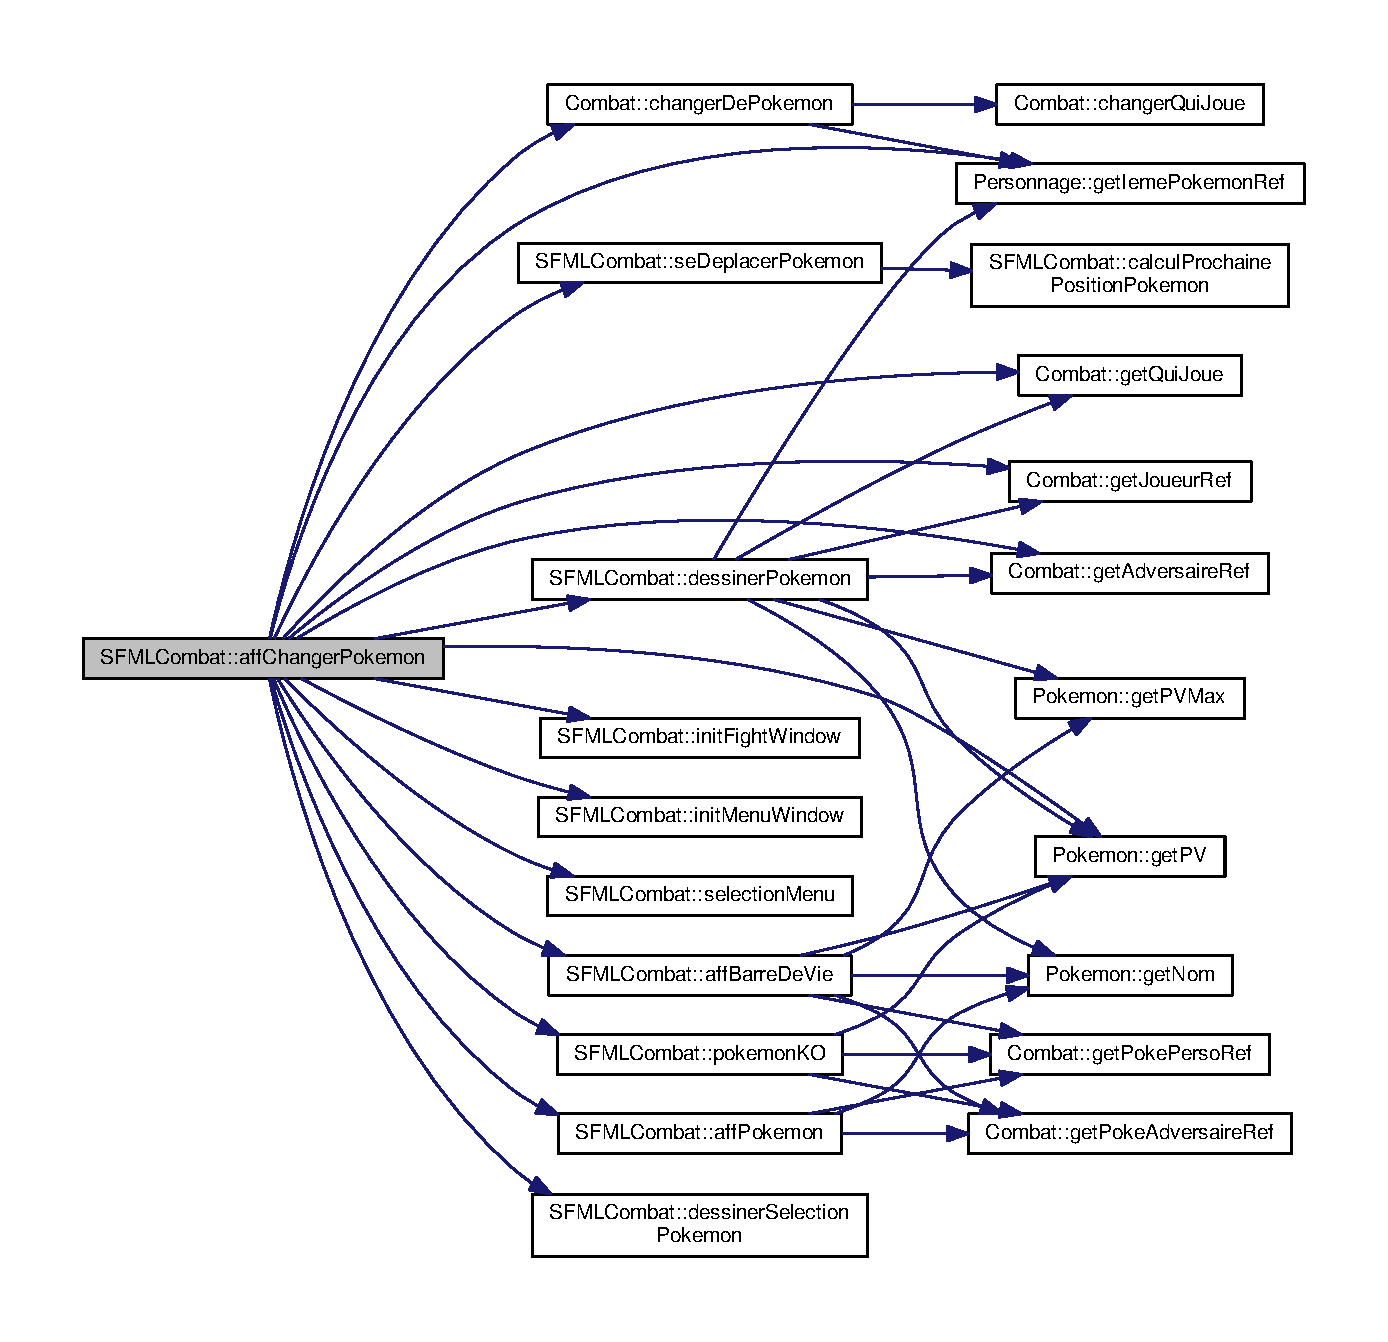
\includegraphics[width=350pt]{class_s_f_m_l_combat_ab8d4dfb3e7e4ca9722e52c1ef5fa897d_cgraph}
\end{center}
\end{figure}
Voici le graphe des appelants de cette fonction \+:\nopagebreak
\begin{figure}[H]
\begin{center}
\leavevmode
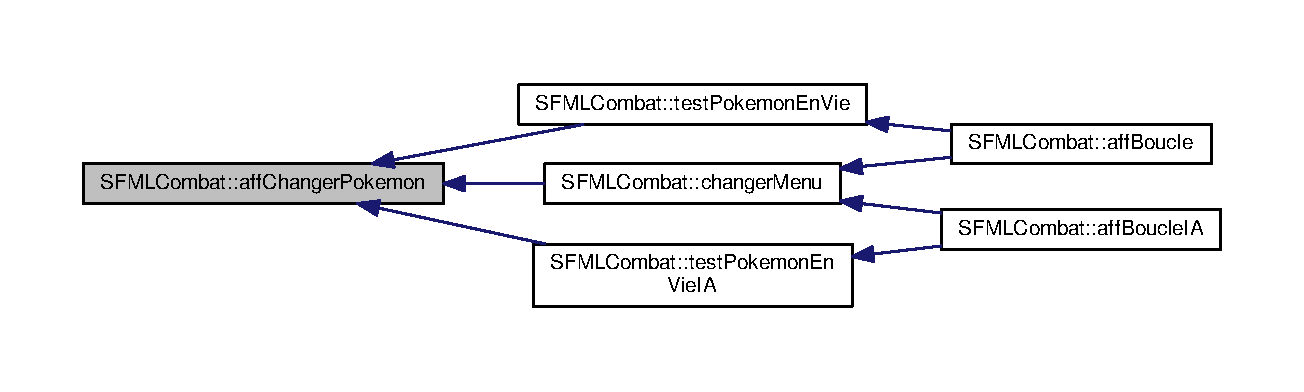
\includegraphics[width=350pt]{class_s_f_m_l_combat_ab8d4dfb3e7e4ca9722e52c1ef5fa897d_icgraph}
\end{center}
\end{figure}
\mbox{\Hypertarget{class_s_f_m_l_combat_a4b2bed6ea12c96a58e55d968b1652597}\label{class_s_f_m_l_combat_a4b2bed6ea12c96a58e55d968b1652597}} 
\index{S\+F\+M\+L\+Combat@{S\+F\+M\+L\+Combat}!aff\+Combat@{aff\+Combat}}
\index{aff\+Combat@{aff\+Combat}!S\+F\+M\+L\+Combat@{S\+F\+M\+L\+Combat}}
\subsubsection{\texorpdfstring{aff\+Combat()}{affCombat()}}
{\footnotesize\ttfamily void S\+F\+M\+L\+Combat\+::aff\+Combat (\begin{DoxyParamCaption}\item[{int \&}]{Choix\+Menu1,  }\item[{int \&}]{Choix\+Bis1,  }\item[{int \&}]{Choix\+Menu2,  }\item[{int \&}]{Choix\+Bis2 }\end{DoxyParamCaption})\hspace{0.3cm}{\ttfamily [private]}}



Boucle d\textquotesingle{}affichage des actions. 

Permet d\textquotesingle{}afficher chaque action effectué par chaque joueur 
\begin{DoxyParams}[1]{Paramètres}
\mbox{\tt out}  & {\em Choix\+Menu1} & Correspond au choix de menu du J1 (Attaquer, Changer de \hyperlink{class_pokemon}{Pokemon} ou Utiliser un \hyperlink{class_objet}{Objet}) \\
\hline
\mbox{\tt out}  & {\em Choix\+Bis1} & Correspond au choix du J1 en fonction du menu, quelle attaque, objet ou \hyperlink{class_pokemon}{Pokemon} \\
\hline
\mbox{\tt out}  & {\em Choix\+Menu2} & Correspond au choix de menu du J2 (Attaquer, Changer de \hyperlink{class_pokemon}{Pokemon} ou Utiliser un \hyperlink{class_objet}{Objet}) \\
\hline
\mbox{\tt out}  & {\em Choix\+Bis2} & Correspond au choix du J2 en fonction du menu, quelle attaque, objet ou \hyperlink{class_pokemon}{Pokemon} \\
\hline
\end{DoxyParams}
Voici le graphe d\textquotesingle{}appel pour cette fonction \+:\nopagebreak
\begin{figure}[H]
\begin{center}
\leavevmode
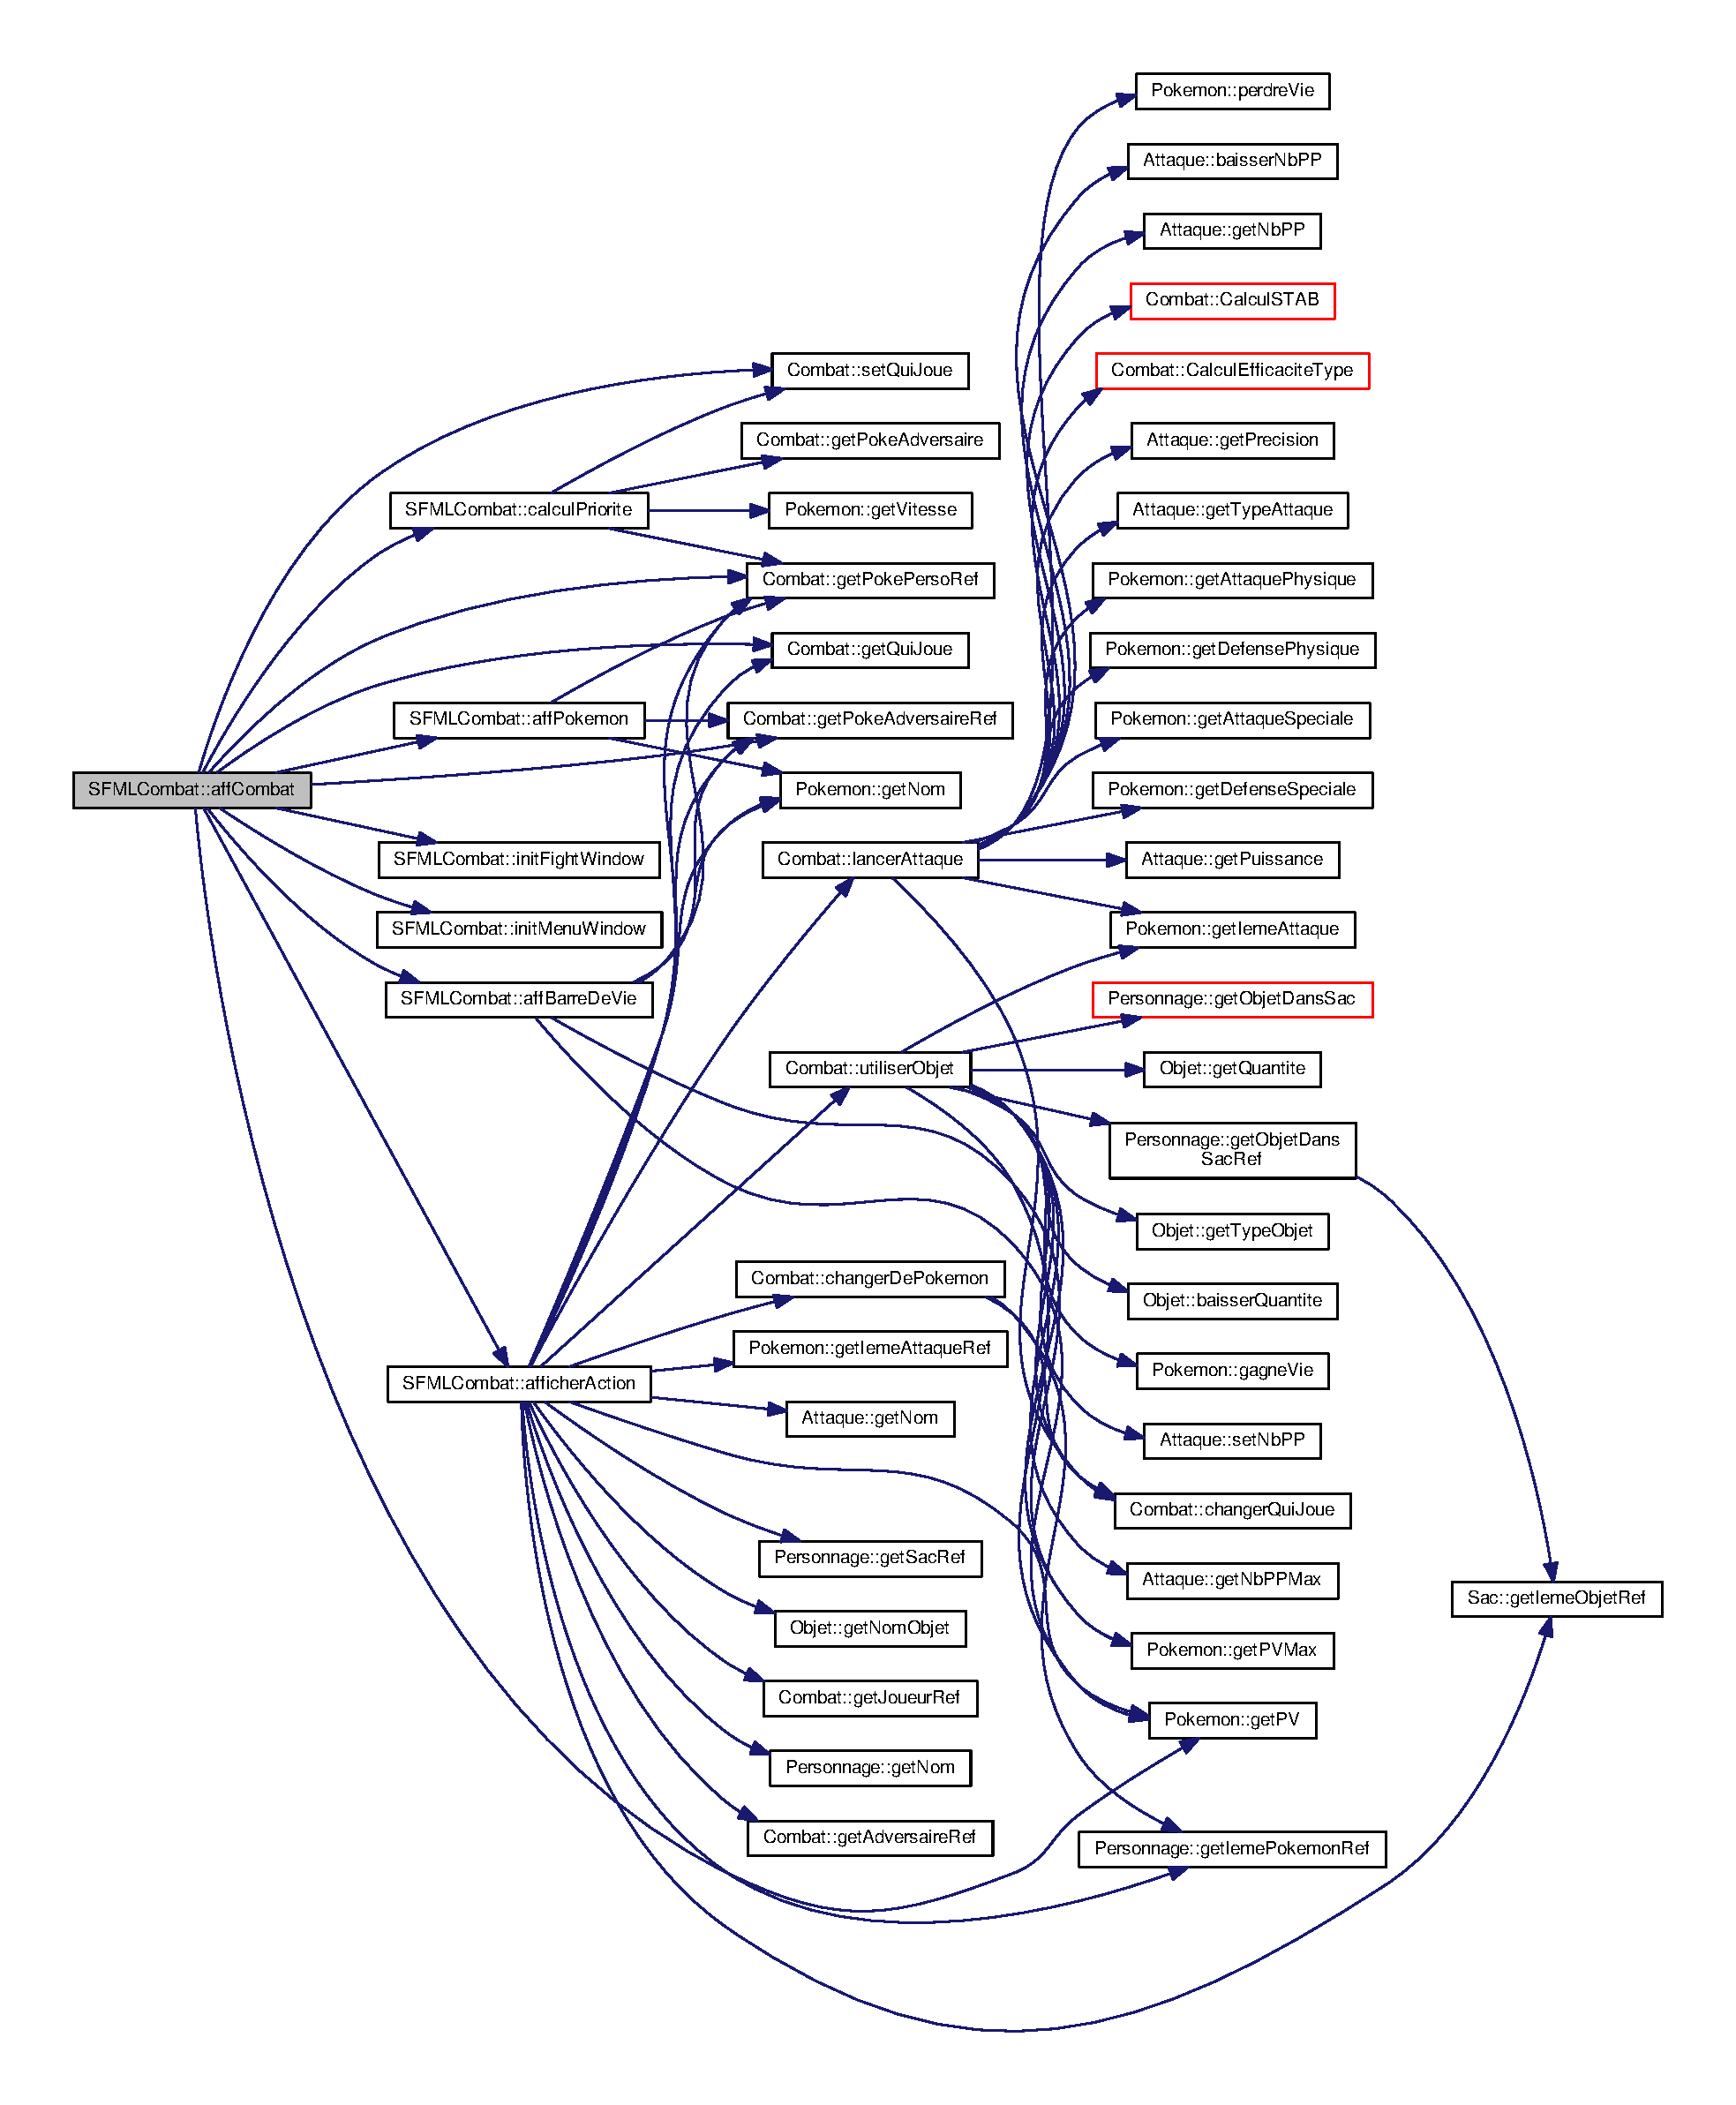
\includegraphics[width=350pt]{class_s_f_m_l_combat_a4b2bed6ea12c96a58e55d968b1652597_cgraph}
\end{center}
\end{figure}
Voici le graphe des appelants de cette fonction \+:\nopagebreak
\begin{figure}[H]
\begin{center}
\leavevmode
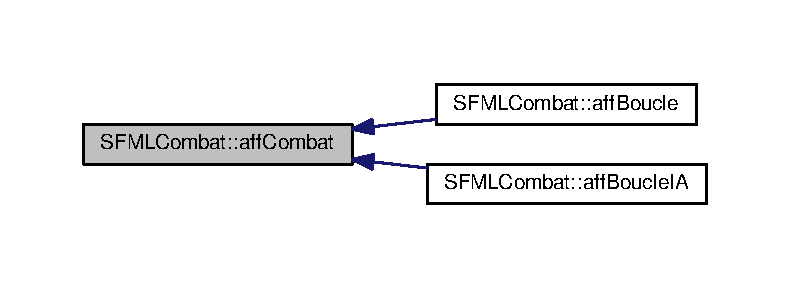
\includegraphics[width=350pt]{class_s_f_m_l_combat_a4b2bed6ea12c96a58e55d968b1652597_icgraph}
\end{center}
\end{figure}
\mbox{\Hypertarget{class_s_f_m_l_combat_ace8cd35d8b2bbc86478a7a28bf0996b4}\label{class_s_f_m_l_combat_ace8cd35d8b2bbc86478a7a28bf0996b4}} 
\index{S\+F\+M\+L\+Combat@{S\+F\+M\+L\+Combat}!aff\+Gagnant@{aff\+Gagnant}}
\index{aff\+Gagnant@{aff\+Gagnant}!S\+F\+M\+L\+Combat@{S\+F\+M\+L\+Combat}}
\subsubsection{\texorpdfstring{aff\+Gagnant()}{affGagnant()}}
{\footnotesize\ttfamily void S\+F\+M\+L\+Combat\+::aff\+Gagnant (\begin{DoxyParamCaption}{ }\end{DoxyParamCaption})\hspace{0.3cm}{\ttfamily [private]}}



Boucle d\textquotesingle{}affichage de fin de partie. 

Gére l\textquotesingle{}affichage de fin de partie Voici le graphe d\textquotesingle{}appel pour cette fonction \+:\nopagebreak
\begin{figure}[H]
\begin{center}
\leavevmode
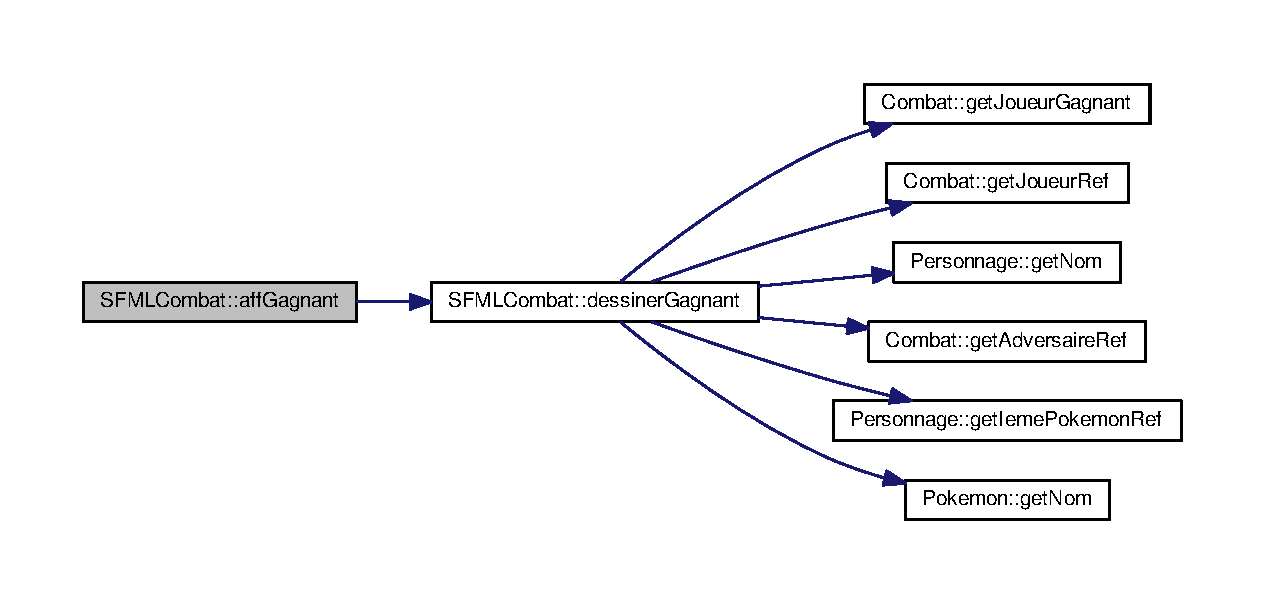
\includegraphics[width=350pt]{class_s_f_m_l_combat_ace8cd35d8b2bbc86478a7a28bf0996b4_cgraph}
\end{center}
\end{figure}
Voici le graphe des appelants de cette fonction \+:\nopagebreak
\begin{figure}[H]
\begin{center}
\leavevmode
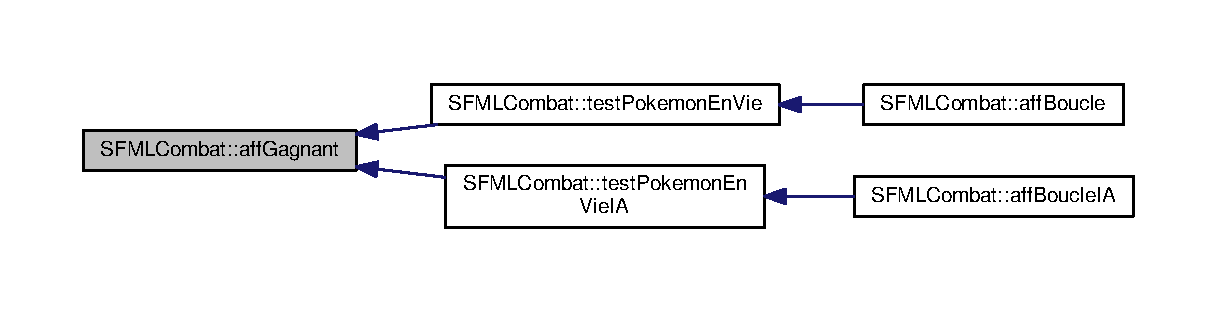
\includegraphics[width=350pt]{class_s_f_m_l_combat_ace8cd35d8b2bbc86478a7a28bf0996b4_icgraph}
\end{center}
\end{figure}
\mbox{\Hypertarget{class_s_f_m_l_combat_acc968da97d4c933f516e67b0356e3d73}\label{class_s_f_m_l_combat_acc968da97d4c933f516e67b0356e3d73}} 
\index{S\+F\+M\+L\+Combat@{S\+F\+M\+L\+Combat}!afficher\+Action@{afficher\+Action}}
\index{afficher\+Action@{afficher\+Action}!S\+F\+M\+L\+Combat@{S\+F\+M\+L\+Combat}}
\subsubsection{\texorpdfstring{afficher\+Action()}{afficherAction()}}
{\footnotesize\ttfamily void S\+F\+M\+L\+Combat\+::afficher\+Action (\begin{DoxyParamCaption}{ }\end{DoxyParamCaption})\hspace{0.3cm}{\ttfamily [private]}}



Affichage textuel des actions effectués. 

Desinne le texte des actions effectués par chaque joueur Voici le graphe d\textquotesingle{}appel pour cette fonction \+:\nopagebreak
\begin{figure}[H]
\begin{center}
\leavevmode
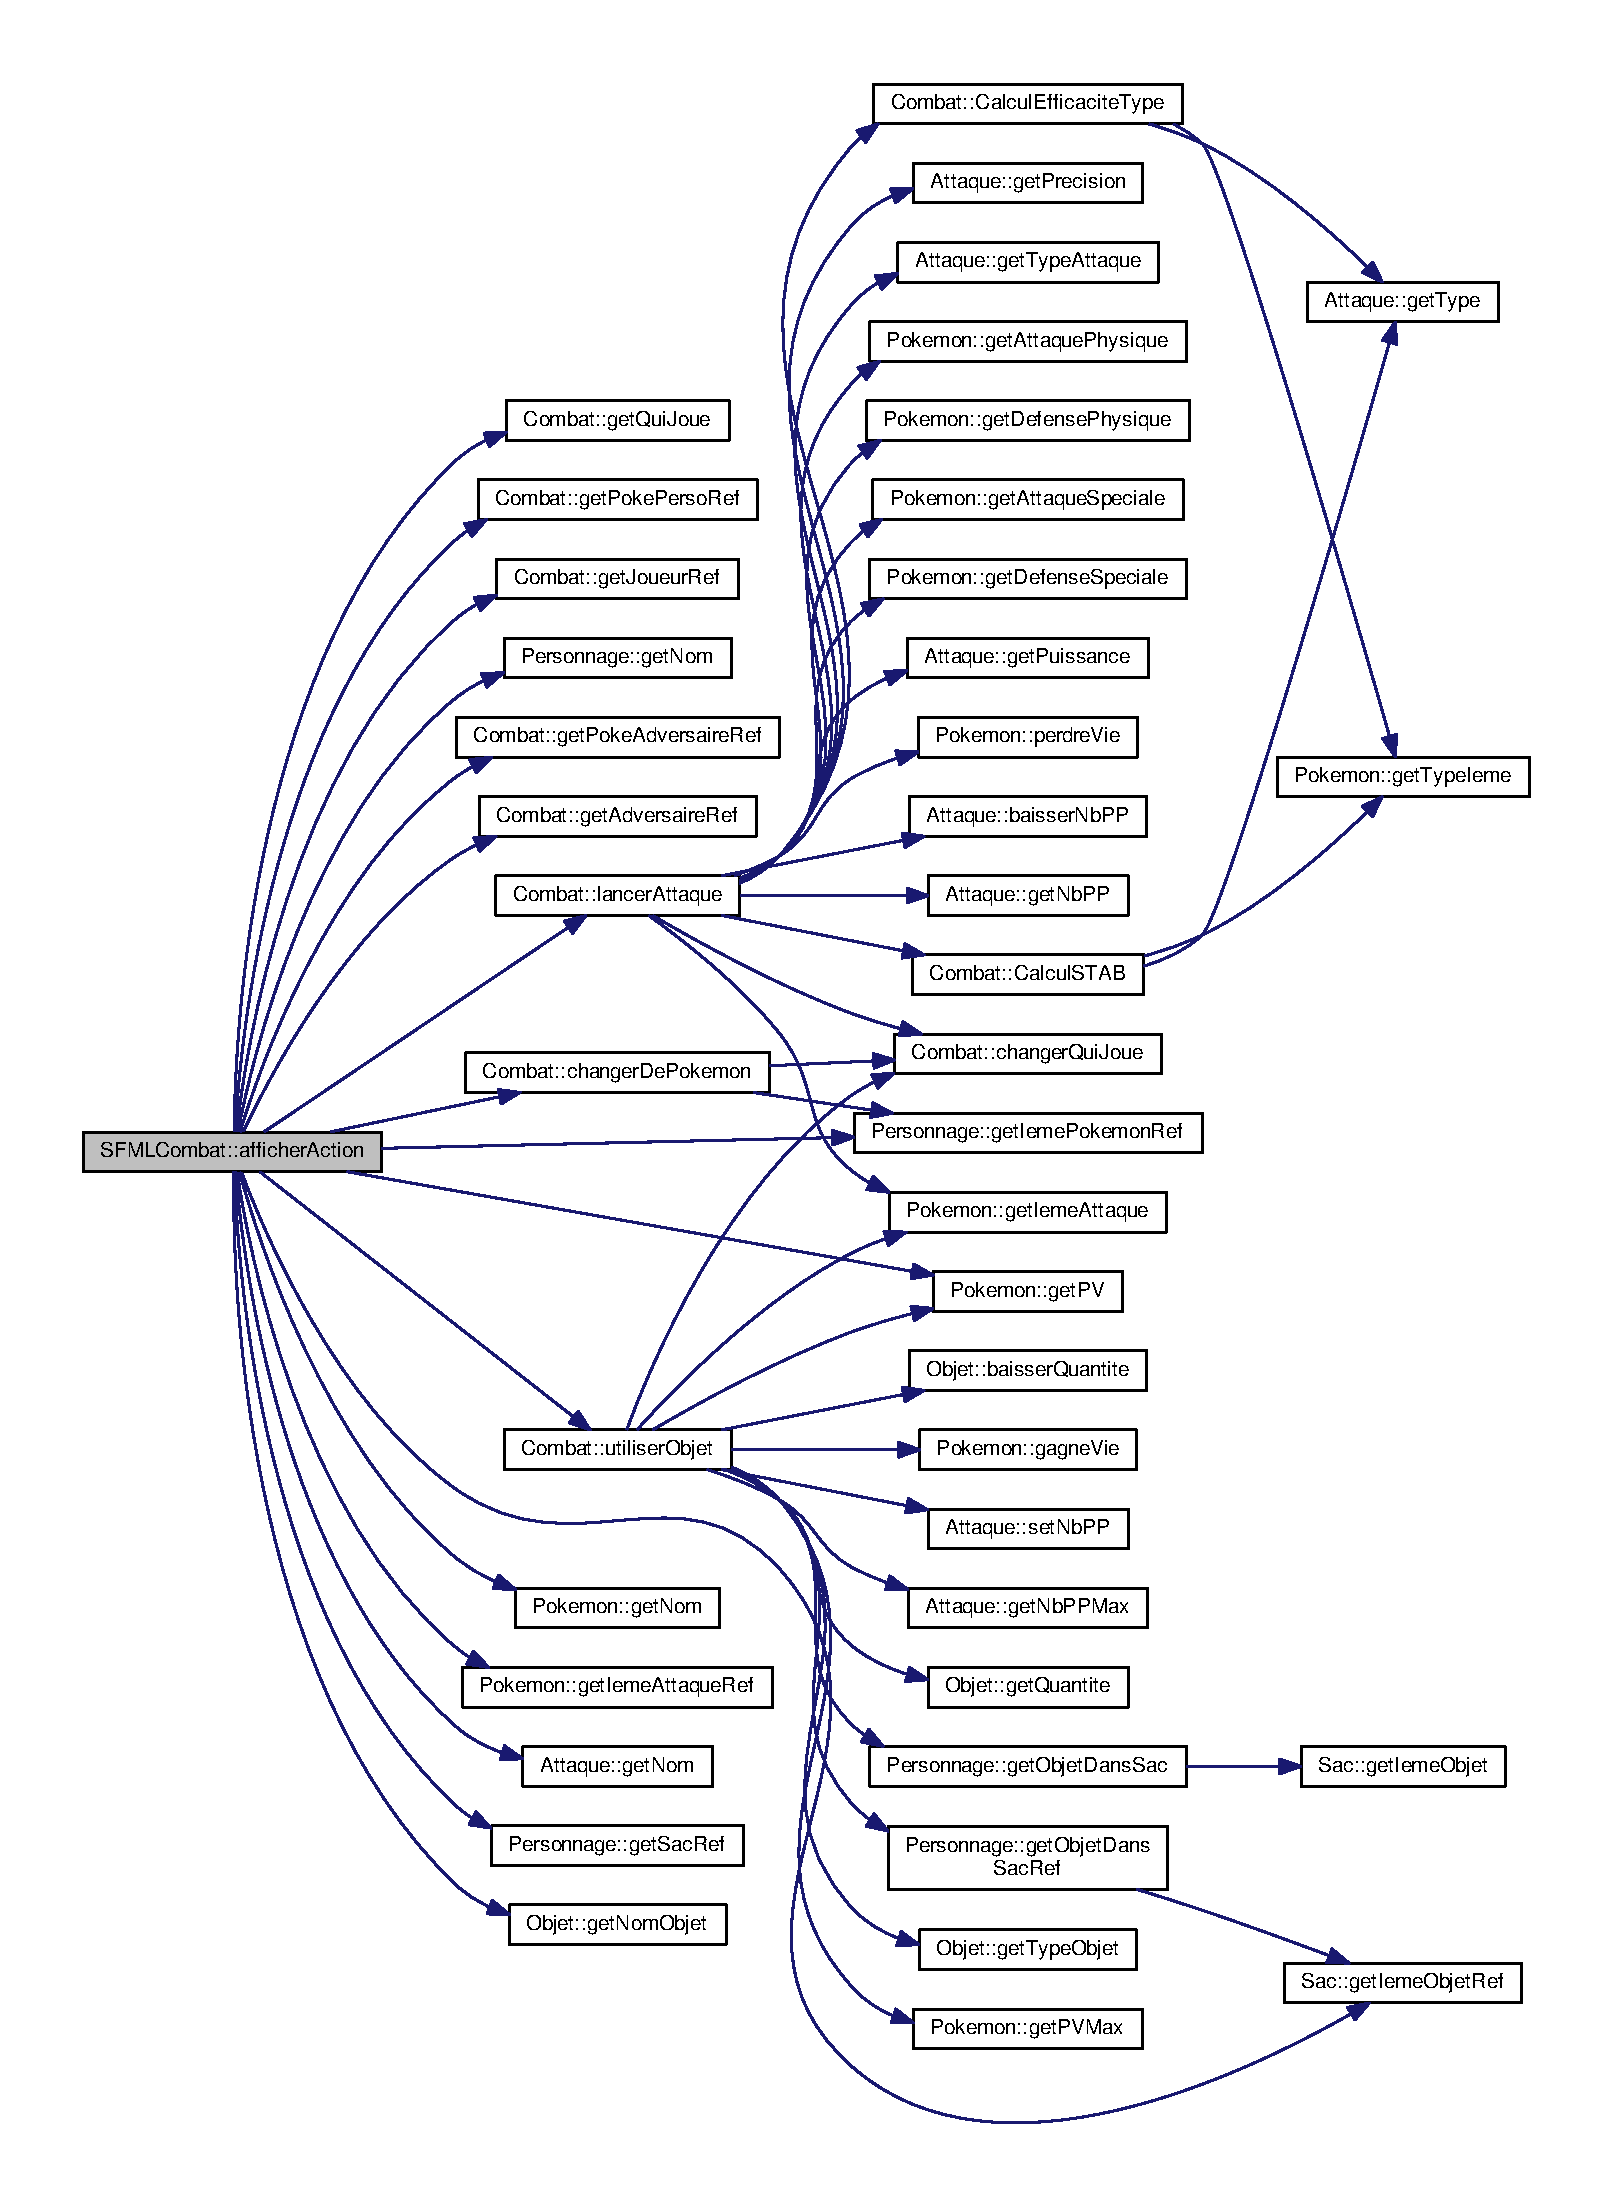
\includegraphics[width=350pt]{class_s_f_m_l_combat_acc968da97d4c933f516e67b0356e3d73_cgraph}
\end{center}
\end{figure}
Voici le graphe des appelants de cette fonction \+:\nopagebreak
\begin{figure}[H]
\begin{center}
\leavevmode
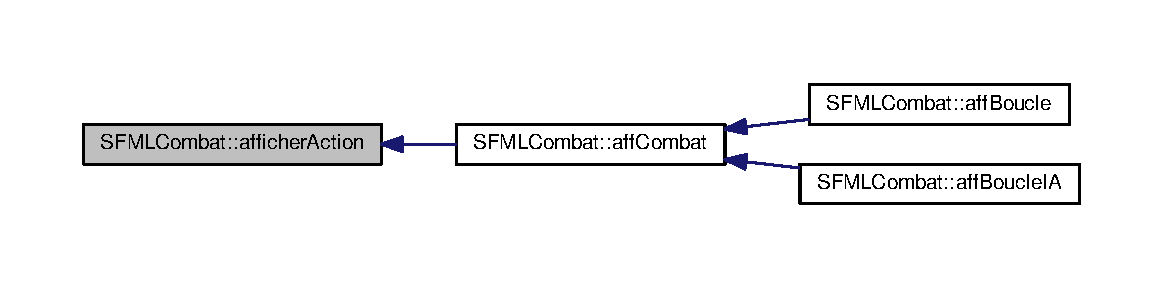
\includegraphics[width=350pt]{class_s_f_m_l_combat_acc968da97d4c933f516e67b0356e3d73_icgraph}
\end{center}
\end{figure}
\mbox{\Hypertarget{class_s_f_m_l_combat_a55c6728be410efdf2ca919a9ee44728a}\label{class_s_f_m_l_combat_a55c6728be410efdf2ca919a9ee44728a}} 
\index{S\+F\+M\+L\+Combat@{S\+F\+M\+L\+Combat}!aff\+Objet@{aff\+Objet}}
\index{aff\+Objet@{aff\+Objet}!S\+F\+M\+L\+Combat@{S\+F\+M\+L\+Combat}}
\subsubsection{\texorpdfstring{aff\+Objet()}{affObjet()}}
{\footnotesize\ttfamily void S\+F\+M\+L\+Combat\+::aff\+Objet (\begin{DoxyParamCaption}{ }\end{DoxyParamCaption})\hspace{0.3cm}{\ttfamily [private]}}



Boucle d\textquotesingle{}affichage du menu objet. 

Permet de gérer le menu d\textquotesingle{}objet, et de gérer la selection d\textquotesingle{}un objet à utiliser Voici le graphe d\textquotesingle{}appel pour cette fonction \+:\nopagebreak
\begin{figure}[H]
\begin{center}
\leavevmode
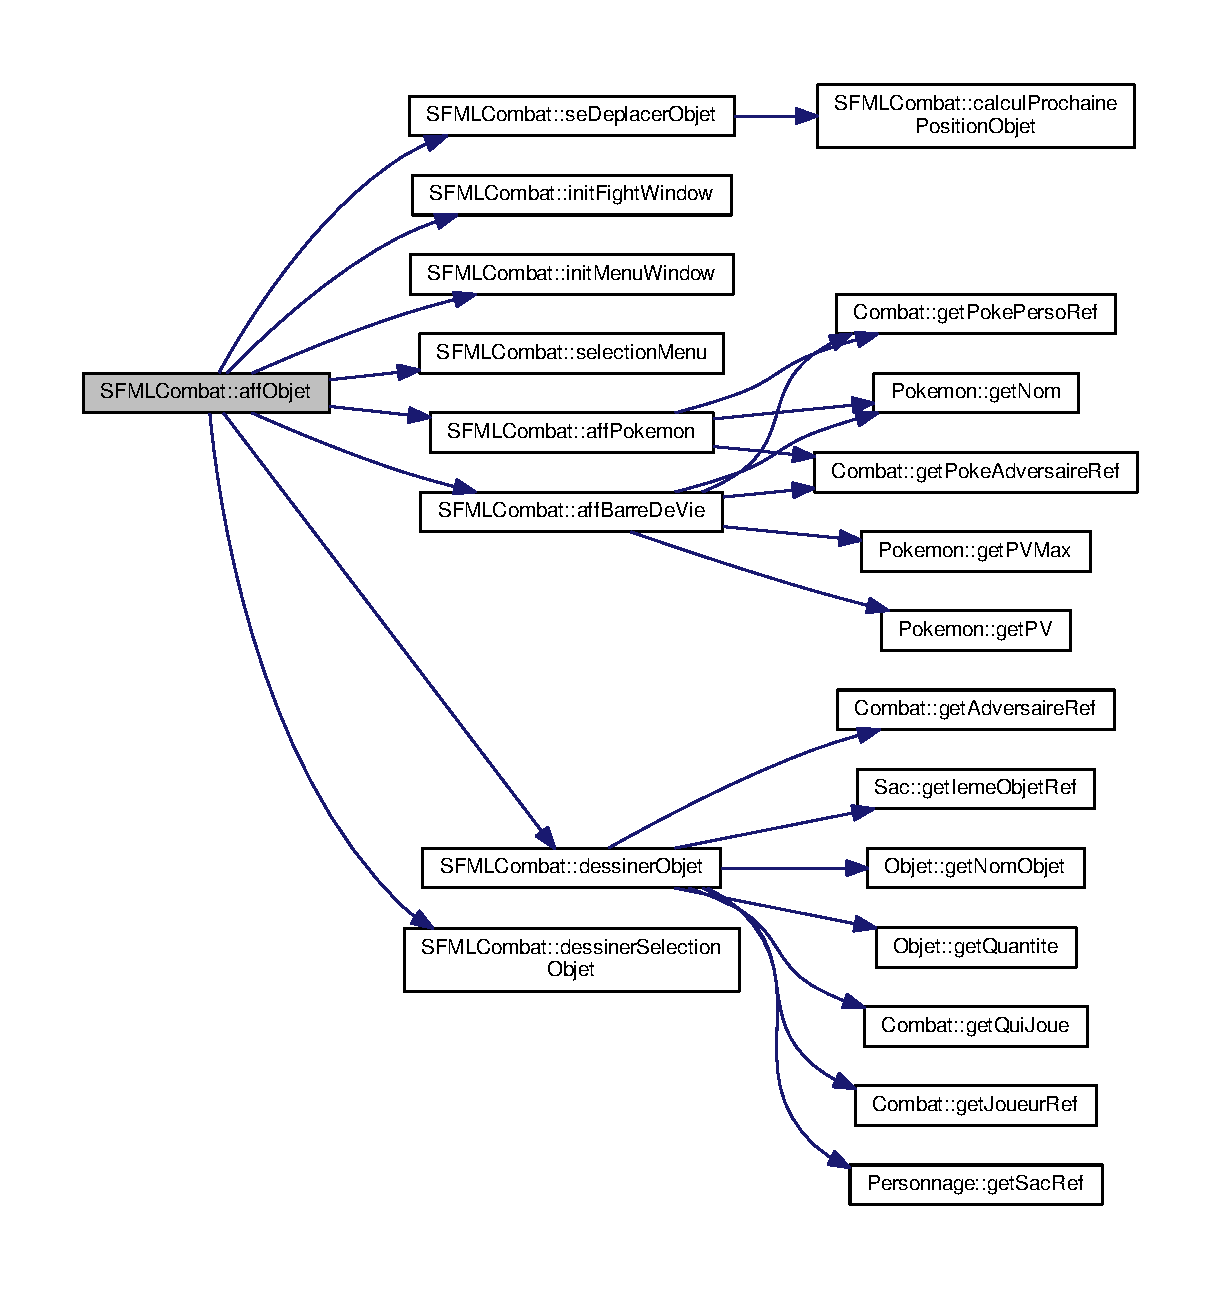
\includegraphics[width=350pt]{class_s_f_m_l_combat_a55c6728be410efdf2ca919a9ee44728a_cgraph}
\end{center}
\end{figure}
Voici le graphe des appelants de cette fonction \+:\nopagebreak
\begin{figure}[H]
\begin{center}
\leavevmode
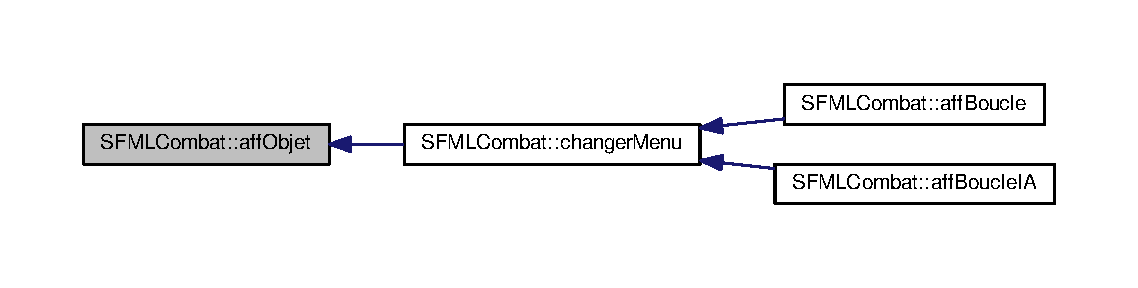
\includegraphics[width=350pt]{class_s_f_m_l_combat_a55c6728be410efdf2ca919a9ee44728a_icgraph}
\end{center}
\end{figure}
\mbox{\Hypertarget{class_s_f_m_l_combat_ab5de8e3048e2549352cea43a3ff636d4}\label{class_s_f_m_l_combat_ab5de8e3048e2549352cea43a3ff636d4}} 
\index{S\+F\+M\+L\+Combat@{S\+F\+M\+L\+Combat}!aff\+Pokemon@{aff\+Pokemon}}
\index{aff\+Pokemon@{aff\+Pokemon}!S\+F\+M\+L\+Combat@{S\+F\+M\+L\+Combat}}
\subsubsection{\texorpdfstring{aff\+Pokemon()}{affPokemon()}}
{\footnotesize\ttfamily void S\+F\+M\+L\+Combat\+::aff\+Pokemon (\begin{DoxyParamCaption}{ }\end{DoxyParamCaption})\hspace{0.3cm}{\ttfamily [private]}}

$\vert$brief Affichage des \hyperlink{class_pokemon}{Pokemon} actuellement en combat

Desinne les sprites des \hyperlink{class_pokemon}{Pokemon} de chaque \hyperlink{class_joueur}{Joueur} étant actuellement en combat Voici le graphe d\textquotesingle{}appel pour cette fonction \+:\nopagebreak
\begin{figure}[H]
\begin{center}
\leavevmode
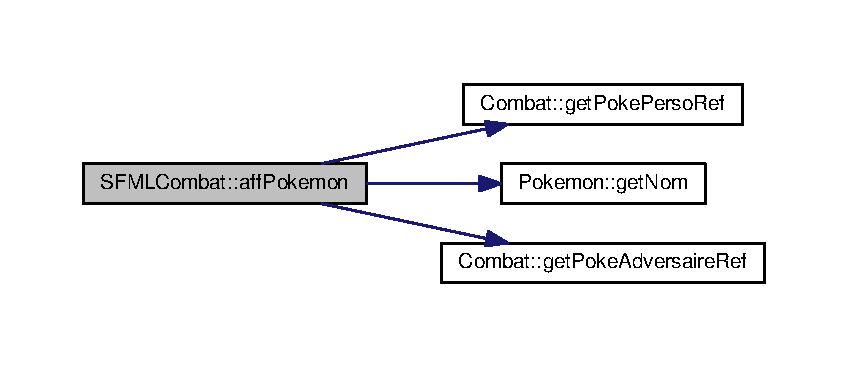
\includegraphics[width=350pt]{class_s_f_m_l_combat_ab5de8e3048e2549352cea43a3ff636d4_cgraph}
\end{center}
\end{figure}
Voici le graphe des appelants de cette fonction \+:\nopagebreak
\begin{figure}[H]
\begin{center}
\leavevmode
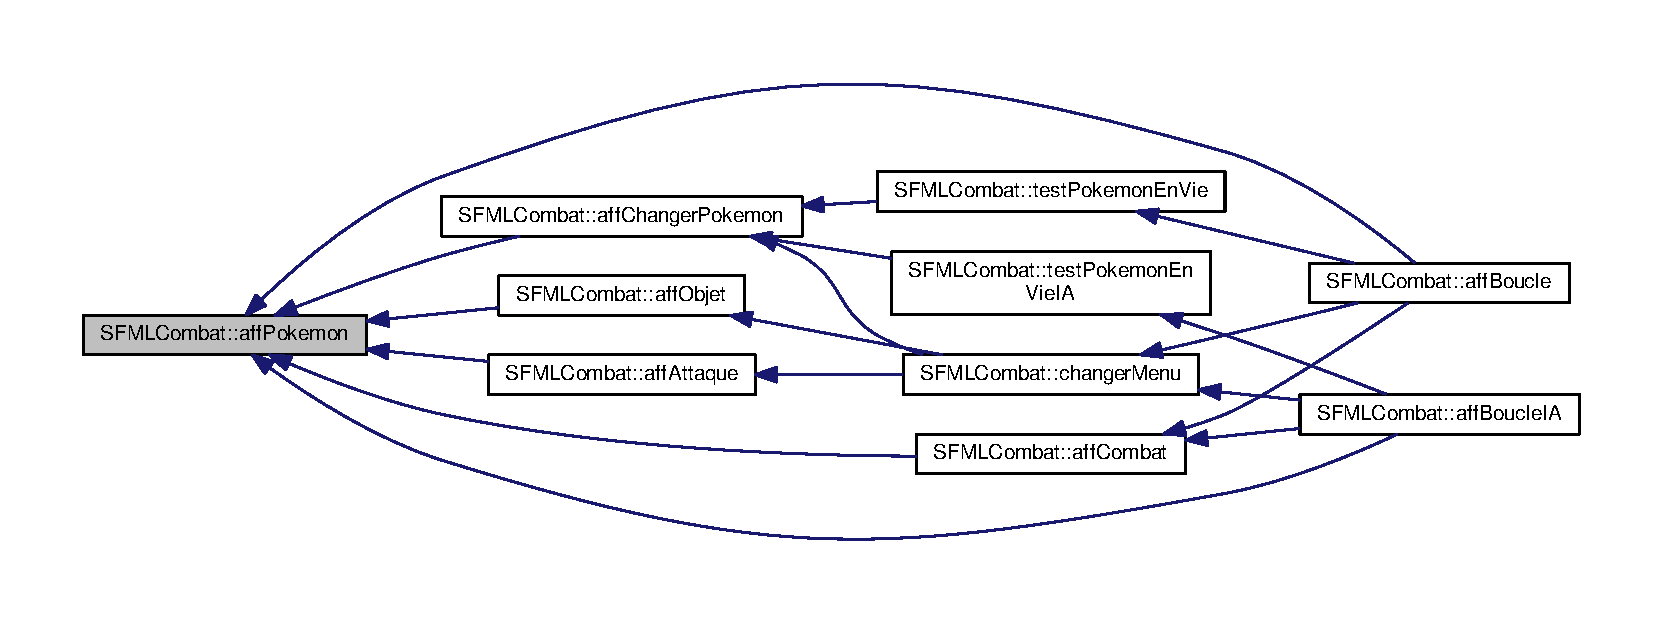
\includegraphics[width=350pt]{class_s_f_m_l_combat_ab5de8e3048e2549352cea43a3ff636d4_icgraph}
\end{center}
\end{figure}
\mbox{\Hypertarget{class_s_f_m_l_combat_ae641a09e3a5a8e50b3fe8352207e4748}\label{class_s_f_m_l_combat_ae641a09e3a5a8e50b3fe8352207e4748}} 
\index{S\+F\+M\+L\+Combat@{S\+F\+M\+L\+Combat}!aff\+Tour@{aff\+Tour}}
\index{aff\+Tour@{aff\+Tour}!S\+F\+M\+L\+Combat@{S\+F\+M\+L\+Combat}}
\subsubsection{\texorpdfstring{aff\+Tour()}{affTour()}}
{\footnotesize\ttfamily void S\+F\+M\+L\+Combat\+::aff\+Tour (\begin{DoxyParamCaption}{ }\end{DoxyParamCaption})\hspace{0.3cm}{\ttfamily [private]}}

$\vert$brief Affichage du tour

Dessine un texte dans le coin supérieure droit permettant de savoir qui doit jouer Voici le graphe d\textquotesingle{}appel pour cette fonction \+:\nopagebreak
\begin{figure}[H]
\begin{center}
\leavevmode
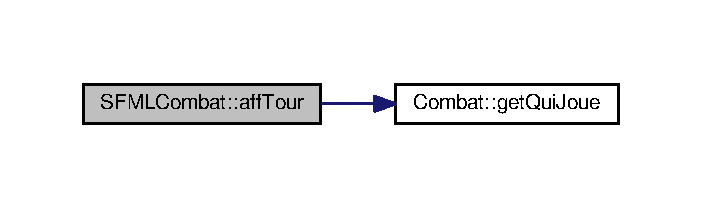
\includegraphics[width=337pt]{class_s_f_m_l_combat_ae641a09e3a5a8e50b3fe8352207e4748_cgraph}
\end{center}
\end{figure}
Voici le graphe des appelants de cette fonction \+:\nopagebreak
\begin{figure}[H]
\begin{center}
\leavevmode
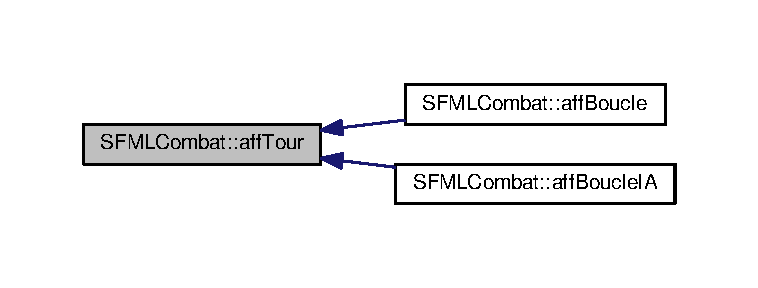
\includegraphics[width=350pt]{class_s_f_m_l_combat_ae641a09e3a5a8e50b3fe8352207e4748_icgraph}
\end{center}
\end{figure}
\mbox{\Hypertarget{class_s_f_m_l_combat_a226dd0d639049753aef1fef95cf9a3f0}\label{class_s_f_m_l_combat_a226dd0d639049753aef1fef95cf9a3f0}} 
\index{S\+F\+M\+L\+Combat@{S\+F\+M\+L\+Combat}!Avantage\+Type@{Avantage\+Type}}
\index{Avantage\+Type@{Avantage\+Type}!S\+F\+M\+L\+Combat@{S\+F\+M\+L\+Combat}}
\subsubsection{\texorpdfstring{Avantage\+Type()}{AvantageType()}}
{\footnotesize\ttfamily float S\+F\+M\+L\+Combat\+::\+Avantage\+Type (\begin{DoxyParamCaption}\item[{const \hyperlink{class_pokemon}{Pokemon} \&}]{Pkmn\+IA,  }\item[{const \hyperlink{_attaque_8h_a1d1cfd8ffb84e947f82999c682b666a7}{Type} \&}]{type\+Joueur }\end{DoxyParamCaption})\hspace{0.3cm}{\ttfamily [private]}}



Calcul l\textquotesingle{}avantage d\textquotesingle{}un type par rapport aux types d\textquotesingle{}un \hyperlink{class_pokemon}{Pokemon}. 

Calcul le multiplicateur de dégâts d\textquotesingle{}un type par rapport a (ou aux) type(s) d\textquotesingle{}un \hyperlink{class_pokemon}{Pokemon} en fonction de résistance et faiblesse du \hyperlink{class_pokemon}{Pokemon} \begin{DoxyReturn}{Renvoie}
Renvoie le multiplicateur de dégâts 
\end{DoxyReturn}
Voici le graphe d\textquotesingle{}appel pour cette fonction \+:\nopagebreak
\begin{figure}[H]
\begin{center}
\leavevmode
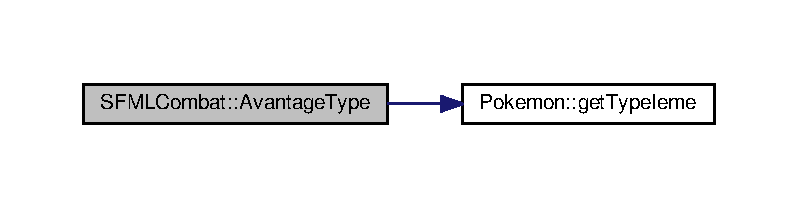
\includegraphics[width=350pt]{class_s_f_m_l_combat_a226dd0d639049753aef1fef95cf9a3f0_cgraph}
\end{center}
\end{figure}
Voici le graphe des appelants de cette fonction \+:\nopagebreak
\begin{figure}[H]
\begin{center}
\leavevmode
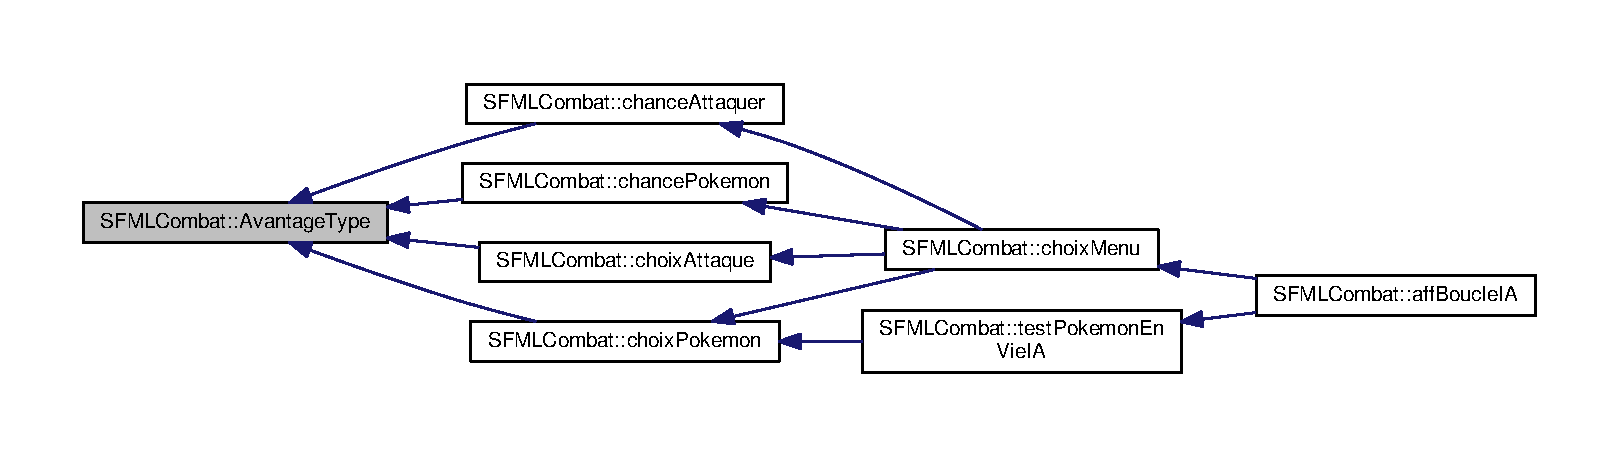
\includegraphics[width=350pt]{class_s_f_m_l_combat_a226dd0d639049753aef1fef95cf9a3f0_icgraph}
\end{center}
\end{figure}
\mbox{\Hypertarget{class_s_f_m_l_combat_af3dbb1374820d004fdf5907397760335}\label{class_s_f_m_l_combat_af3dbb1374820d004fdf5907397760335}} 
\index{S\+F\+M\+L\+Combat@{S\+F\+M\+L\+Combat}!calcul\+Priorite@{calcul\+Priorite}}
\index{calcul\+Priorite@{calcul\+Priorite}!S\+F\+M\+L\+Combat@{S\+F\+M\+L\+Combat}}
\subsubsection{\texorpdfstring{calcul\+Priorite()}{calculPriorite()}}
{\footnotesize\ttfamily void S\+F\+M\+L\+Combat\+::calcul\+Priorite (\begin{DoxyParamCaption}\item[{int}]{Choix\+Menu1,  }\item[{int}]{Choix\+Bis1,  }\item[{int}]{Choix\+Menu2,  }\item[{int}]{Choix\+Bis2 }\end{DoxyParamCaption})\hspace{0.3cm}{\ttfamily [private]}}



Calcul de la priorité des Joueurs. 

Calcul quel joueur a la priorité sur l\textquotesingle{}autre en fonction des actions choisies ainsi que des statistiques de chaque \hyperlink{class_pokemon}{Pokemon} 
\begin{DoxyParams}[1]{Paramètres}
\mbox{\tt in}  & {\em Choix\+Menu1} & Correspond au choix de menu du J1 (Attaquer, Changer de \hyperlink{class_pokemon}{Pokemon} ou Utiliser un \hyperlink{class_objet}{Objet}) \\
\hline
\mbox{\tt in}  & {\em Choix\+Bis1} & Correspond au choix du J1 en fonction du menu, quelle attaque, objet ou \hyperlink{class_pokemon}{Pokemon} \\
\hline
\mbox{\tt in}  & {\em Choix\+Menu2} & Correspond au choix de menu du J2 (Attaquer, Changer de \hyperlink{class_pokemon}{Pokemon} ou Utiliser un \hyperlink{class_objet}{Objet}) \\
\hline
\mbox{\tt in}  & {\em Choix\+Bis2} & Correspond au choix du J2 en fonction du menu, quelle attaque, objet ou \hyperlink{class_pokemon}{Pokemon} \\
\hline
\end{DoxyParams}
Voici le graphe d\textquotesingle{}appel pour cette fonction \+:\nopagebreak
\begin{figure}[H]
\begin{center}
\leavevmode
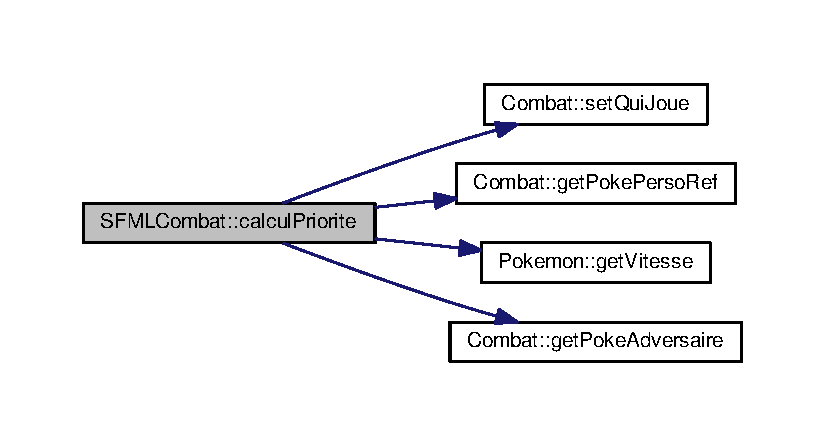
\includegraphics[width=350pt]{class_s_f_m_l_combat_af3dbb1374820d004fdf5907397760335_cgraph}
\end{center}
\end{figure}
Voici le graphe des appelants de cette fonction \+:\nopagebreak
\begin{figure}[H]
\begin{center}
\leavevmode
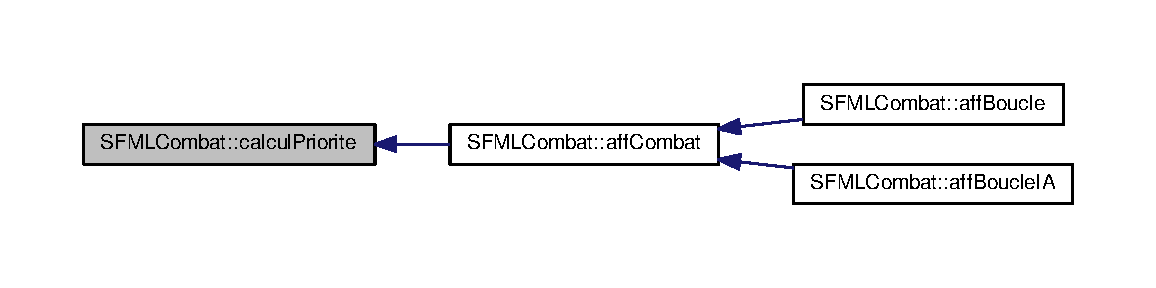
\includegraphics[width=350pt]{class_s_f_m_l_combat_af3dbb1374820d004fdf5907397760335_icgraph}
\end{center}
\end{figure}
\mbox{\Hypertarget{class_s_f_m_l_combat_a2e7feee45aae418d7545cc71534e6148}\label{class_s_f_m_l_combat_a2e7feee45aae418d7545cc71534e6148}} 
\index{S\+F\+M\+L\+Combat@{S\+F\+M\+L\+Combat}!calcul\+Prochaine\+Position@{calcul\+Prochaine\+Position}}
\index{calcul\+Prochaine\+Position@{calcul\+Prochaine\+Position}!S\+F\+M\+L\+Combat@{S\+F\+M\+L\+Combat}}
\subsubsection{\texorpdfstring{calcul\+Prochaine\+Position()}{calculProchainePosition()}}
{\footnotesize\ttfamily int S\+F\+M\+L\+Combat\+::calcul\+Prochaine\+Position (\begin{DoxyParamCaption}\item[{sf\+::\+Event}]{event }\end{DoxyParamCaption})\hspace{0.3cm}{\ttfamily [private]}}

$\vert$brief Calcul de la prochaine position du curseur

Calcul de la prochaine position du curseur en foncton de la touche directionelle préssé par l\textquotesingle{}utilisateur ou renvoie la même position si le déplacement n\textquotesingle{}est pas autorisé 
\begin{DoxyParams}[1]{Paramètres}
\mbox{\tt in}  & {\em event} & Correspond à la touche directionelle préssé par l\textquotesingle{}utilisateur \\
\hline
\end{DoxyParams}
Voici le graphe des appelants de cette fonction \+:\nopagebreak
\begin{figure}[H]
\begin{center}
\leavevmode
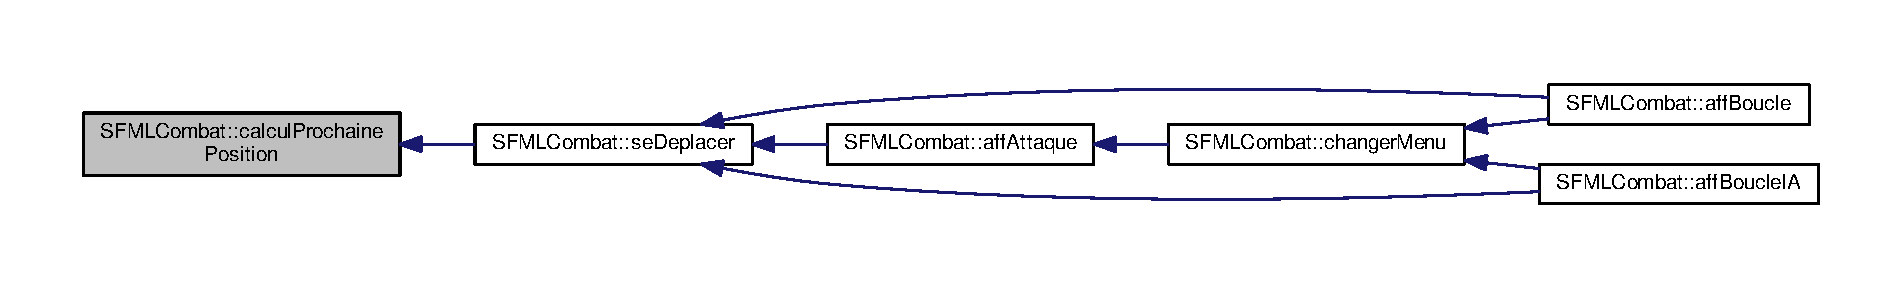
\includegraphics[width=350pt]{class_s_f_m_l_combat_a2e7feee45aae418d7545cc71534e6148_icgraph}
\end{center}
\end{figure}
\mbox{\Hypertarget{class_s_f_m_l_combat_a06e5c66f031d48316b7d779a9589c18e}\label{class_s_f_m_l_combat_a06e5c66f031d48316b7d779a9589c18e}} 
\index{S\+F\+M\+L\+Combat@{S\+F\+M\+L\+Combat}!calcul\+Prochaine\+Position\+Objet@{calcul\+Prochaine\+Position\+Objet}}
\index{calcul\+Prochaine\+Position\+Objet@{calcul\+Prochaine\+Position\+Objet}!S\+F\+M\+L\+Combat@{S\+F\+M\+L\+Combat}}
\subsubsection{\texorpdfstring{calcul\+Prochaine\+Position\+Objet()}{calculProchainePositionObjet()}}
{\footnotesize\ttfamily int S\+F\+M\+L\+Combat\+::calcul\+Prochaine\+Position\+Objet (\begin{DoxyParamCaption}\item[{sf\+::\+Event}]{event,  }\item[{int}]{position\+Objet }\end{DoxyParamCaption})\hspace{0.3cm}{\ttfamily [private]}}



Calcul de la prochaine position objet. 

Permet de calculer la prochaine position de l\textquotesingle{}objet en fonction de la touche directionelle préssé 
\begin{DoxyParams}[1]{Paramètres}
\mbox{\tt in}  & {\em position\+Objet} & Index de position de l\textquotesingle{}objet étant actuellement pointé par le curseur \\
\hline
\mbox{\tt in}  & {\em event} & Correspond à la touche qui est préssé par l\textquotesingle{}utilisateur \\
\hline
\end{DoxyParams}
\begin{DoxyReturn}{Renvoie}
Renvoie la future position du curseur sur objet, ou la même position que précédemment si le déplacement n\textquotesingle{}est pas autorisé 
\end{DoxyReturn}
Voici le graphe des appelants de cette fonction \+:\nopagebreak
\begin{figure}[H]
\begin{center}
\leavevmode
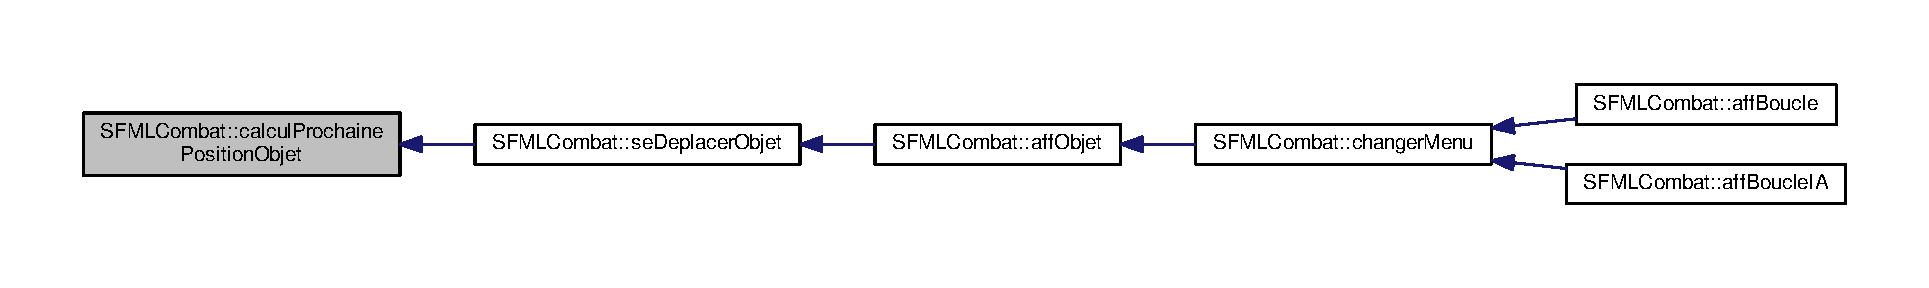
\includegraphics[width=350pt]{class_s_f_m_l_combat_a06e5c66f031d48316b7d779a9589c18e_icgraph}
\end{center}
\end{figure}
\mbox{\Hypertarget{class_s_f_m_l_combat_ab0728cc1b2fcc52112165ec8e3e14eb6}\label{class_s_f_m_l_combat_ab0728cc1b2fcc52112165ec8e3e14eb6}} 
\index{S\+F\+M\+L\+Combat@{S\+F\+M\+L\+Combat}!calcul\+Prochaine\+Position\+Pokemon@{calcul\+Prochaine\+Position\+Pokemon}}
\index{calcul\+Prochaine\+Position\+Pokemon@{calcul\+Prochaine\+Position\+Pokemon}!S\+F\+M\+L\+Combat@{S\+F\+M\+L\+Combat}}
\subsubsection{\texorpdfstring{calcul\+Prochaine\+Position\+Pokemon()}{calculProchainePositionPokemon()}}
{\footnotesize\ttfamily int S\+F\+M\+L\+Combat\+::calcul\+Prochaine\+Position\+Pokemon (\begin{DoxyParamCaption}\item[{sf\+::\+Event}]{event,  }\item[{int}]{position\+Pokemon }\end{DoxyParamCaption})\hspace{0.3cm}{\ttfamily [private]}}



Calcul de la prochaine position \hyperlink{class_pokemon}{Pokemon}. 

Permet de calculer la prochaine position du cursueur sur \hyperlink{class_pokemon}{Pokemon} en fonction de la touche directionelle préssé 
\begin{DoxyParams}[1]{Paramètres}
\mbox{\tt in}  & {\em position\+Pokemon} & Index de position du \hyperlink{class_pokemon}{Pokemon} étant actuellement pointé par le curseur \\
\hline
\mbox{\tt in}  & {\em event} & Correspond à la touche qui est préssé par l\textquotesingle{}utilisateur \\
\hline
\end{DoxyParams}
\begin{DoxyReturn}{Renvoie}
Renvoie la future position du curseur sur objet, ou la même position que précédemment si le déplacement n\textquotesingle{}est pas autorisé 
\end{DoxyReturn}
Voici le graphe des appelants de cette fonction \+:\nopagebreak
\begin{figure}[H]
\begin{center}
\leavevmode
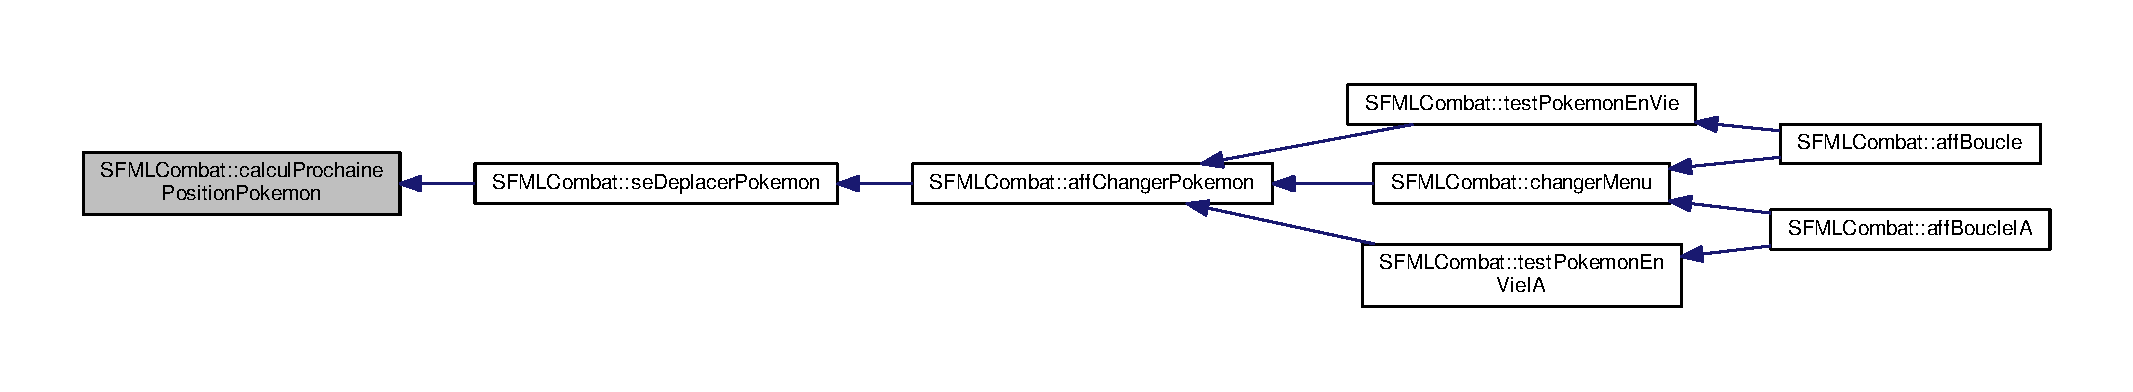
\includegraphics[width=350pt]{class_s_f_m_l_combat_ab0728cc1b2fcc52112165ec8e3e14eb6_icgraph}
\end{center}
\end{figure}
\mbox{\Hypertarget{class_s_f_m_l_combat_ac8720bfe637fdaa932ef45240493bbd6}\label{class_s_f_m_l_combat_ac8720bfe637fdaa932ef45240493bbd6}} 
\index{S\+F\+M\+L\+Combat@{S\+F\+M\+L\+Combat}!chance\+Attaquer@{chance\+Attaquer}}
\index{chance\+Attaquer@{chance\+Attaquer}!S\+F\+M\+L\+Combat@{S\+F\+M\+L\+Combat}}
\subsubsection{\texorpdfstring{chance\+Attaquer()}{chanceAttaquer()}}
{\footnotesize\ttfamily bool S\+F\+M\+L\+Combat\+::chance\+Attaquer (\begin{DoxyParamCaption}{ }\end{DoxyParamCaption})\hspace{0.3cm}{\ttfamily [private]}}



Chance d\textquotesingle{}attaquer. 

Effectue différent test afin de savoir si il faut attaquer \begin{DoxyReturn}{Renvoie}
Un booléen permettant de savoir si l\textquotesingle{}IA doit attaquer 
\end{DoxyReturn}
Voici le graphe d\textquotesingle{}appel pour cette fonction \+:\nopagebreak
\begin{figure}[H]
\begin{center}
\leavevmode
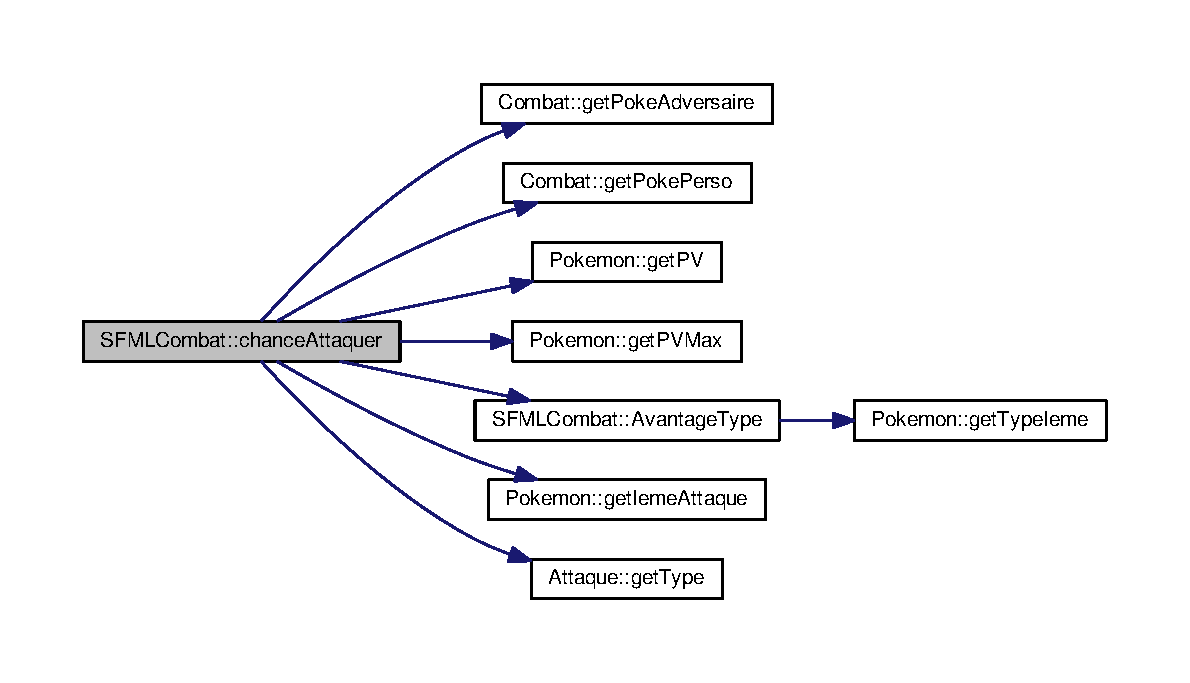
\includegraphics[width=350pt]{class_s_f_m_l_combat_ac8720bfe637fdaa932ef45240493bbd6_cgraph}
\end{center}
\end{figure}
Voici le graphe des appelants de cette fonction \+:\nopagebreak
\begin{figure}[H]
\begin{center}
\leavevmode
\includegraphics[width=350pt]{class_s_f_m_l_combat_ac8720bfe637fdaa932ef45240493bbd6_icgraph}
\end{center}
\end{figure}
\mbox{\Hypertarget{class_s_f_m_l_combat_a00370ff45d848befb5d35c52bd1db2d5}\label{class_s_f_m_l_combat_a00370ff45d848befb5d35c52bd1db2d5}} 
\index{S\+F\+M\+L\+Combat@{S\+F\+M\+L\+Combat}!chance\+Objet@{chance\+Objet}}
\index{chance\+Objet@{chance\+Objet}!S\+F\+M\+L\+Combat@{S\+F\+M\+L\+Combat}}
\subsubsection{\texorpdfstring{chance\+Objet()}{chanceObjet()}}
{\footnotesize\ttfamily bool S\+F\+M\+L\+Combat\+::chance\+Objet (\begin{DoxyParamCaption}{ }\end{DoxyParamCaption})\hspace{0.3cm}{\ttfamily [private]}}



Chance d\textquotesingle{}utiliser un objet. 

Effectue différent test afin de savoir si il faut utiliser un objet \begin{DoxyReturn}{Renvoie}
Un booléen permettant de savoir si l\textquotesingle{}IA doit utiliser un objet 
\end{DoxyReturn}
Voici le graphe d\textquotesingle{}appel pour cette fonction \+:\nopagebreak
\begin{figure}[H]
\begin{center}
\leavevmode
\includegraphics[width=350pt]{class_s_f_m_l_combat_a00370ff45d848befb5d35c52bd1db2d5_cgraph}
\end{center}
\end{figure}
Voici le graphe des appelants de cette fonction \+:\nopagebreak
\begin{figure}[H]
\begin{center}
\leavevmode
\includegraphics[width=350pt]{class_s_f_m_l_combat_a00370ff45d848befb5d35c52bd1db2d5_icgraph}
\end{center}
\end{figure}
\mbox{\Hypertarget{class_s_f_m_l_combat_a4ba9a6e1f0c91eb425ac83649e443375}\label{class_s_f_m_l_combat_a4ba9a6e1f0c91eb425ac83649e443375}} 
\index{S\+F\+M\+L\+Combat@{S\+F\+M\+L\+Combat}!chance\+Pokemon@{chance\+Pokemon}}
\index{chance\+Pokemon@{chance\+Pokemon}!S\+F\+M\+L\+Combat@{S\+F\+M\+L\+Combat}}
\subsubsection{\texorpdfstring{chance\+Pokemon()}{chancePokemon()}}
{\footnotesize\ttfamily bool S\+F\+M\+L\+Combat\+::chance\+Pokemon (\begin{DoxyParamCaption}{ }\end{DoxyParamCaption})\hspace{0.3cm}{\ttfamily [private]}}



Chance de changer de \hyperlink{class_pokemon}{Pokemon}. 

Effectue différent test afin de savoir si il faut utiliser un objet \begin{DoxyReturn}{Renvoie}
Un booléen permettant de savoir si l\textquotesingle{}IA doit utiliser un objet 
\end{DoxyReturn}
Voici le graphe d\textquotesingle{}appel pour cette fonction \+:\nopagebreak
\begin{figure}[H]
\begin{center}
\leavevmode
\includegraphics[width=350pt]{class_s_f_m_l_combat_a4ba9a6e1f0c91eb425ac83649e443375_cgraph}
\end{center}
\end{figure}
Voici le graphe des appelants de cette fonction \+:\nopagebreak
\begin{figure}[H]
\begin{center}
\leavevmode
\includegraphics[width=350pt]{class_s_f_m_l_combat_a4ba9a6e1f0c91eb425ac83649e443375_icgraph}
\end{center}
\end{figure}
\mbox{\Hypertarget{class_s_f_m_l_combat_ab856672c59db95d55c7c28cd3a1eee93}\label{class_s_f_m_l_combat_ab856672c59db95d55c7c28cd3a1eee93}} 
\index{S\+F\+M\+L\+Combat@{S\+F\+M\+L\+Combat}!changer\+Menu@{changer\+Menu}}
\index{changer\+Menu@{changer\+Menu}!S\+F\+M\+L\+Combat@{S\+F\+M\+L\+Combat}}
\subsubsection{\texorpdfstring{changer\+Menu()}{changerMenu()}}
{\footnotesize\ttfamily int S\+F\+M\+L\+Combat\+::changer\+Menu (\begin{DoxyParamCaption}{ }\end{DoxyParamCaption})\hspace{0.3cm}{\ttfamily [private]}}

$\vert$brief Gére le changement de menu

Sélectionne dans quel boucle de menu le programme doit rentrer en fonction du choix de l\textquotesingle{}utilisateur \begin{DoxyReturn}{Renvoie}
Renvoie l\textquotesingle{}indice du menu sélectionné par le joueur 
\end{DoxyReturn}
Voici le graphe d\textquotesingle{}appel pour cette fonction \+:\nopagebreak
\begin{figure}[H]
\begin{center}
\leavevmode
\includegraphics[width=350pt]{class_s_f_m_l_combat_ab856672c59db95d55c7c28cd3a1eee93_cgraph}
\end{center}
\end{figure}
Voici le graphe des appelants de cette fonction \+:\nopagebreak
\begin{figure}[H]
\begin{center}
\leavevmode
\includegraphics[width=350pt]{class_s_f_m_l_combat_ab856672c59db95d55c7c28cd3a1eee93_icgraph}
\end{center}
\end{figure}
\mbox{\Hypertarget{class_s_f_m_l_combat_ab1f7a0fa82f0cfd9c0a0e1c321f5f7e7}\label{class_s_f_m_l_combat_ab1f7a0fa82f0cfd9c0a0e1c321f5f7e7}} 
\index{S\+F\+M\+L\+Combat@{S\+F\+M\+L\+Combat}!choix\+Attaque@{choix\+Attaque}}
\index{choix\+Attaque@{choix\+Attaque}!S\+F\+M\+L\+Combat@{S\+F\+M\+L\+Combat}}
\subsubsection{\texorpdfstring{choix\+Attaque()}{choixAttaque()}}
{\footnotesize\ttfamily int S\+F\+M\+L\+Combat\+::choix\+Attaque (\begin{DoxyParamCaption}{ }\end{DoxyParamCaption})\hspace{0.3cm}{\ttfamily [private]}}



Choix de l\textquotesingle{}attaque à lancer. 

Effectuent différents test pour savoir quelle attaque doit-\/être lancer \begin{DoxyReturn}{Renvoie}
L\textquotesingle{}indice de l\textquotesingle{}attaque à lancer 
\end{DoxyReturn}
Voici le graphe d\textquotesingle{}appel pour cette fonction \+:\nopagebreak
\begin{figure}[H]
\begin{center}
\leavevmode
\includegraphics[width=350pt]{class_s_f_m_l_combat_ab1f7a0fa82f0cfd9c0a0e1c321f5f7e7_cgraph}
\end{center}
\end{figure}
Voici le graphe des appelants de cette fonction \+:\nopagebreak
\begin{figure}[H]
\begin{center}
\leavevmode
\includegraphics[width=350pt]{class_s_f_m_l_combat_ab1f7a0fa82f0cfd9c0a0e1c321f5f7e7_icgraph}
\end{center}
\end{figure}
\mbox{\Hypertarget{class_s_f_m_l_combat_ad72f480db9eb3f134e3736b1acb228c8}\label{class_s_f_m_l_combat_ad72f480db9eb3f134e3736b1acb228c8}} 
\index{S\+F\+M\+L\+Combat@{S\+F\+M\+L\+Combat}!choix\+Menu@{choix\+Menu}}
\index{choix\+Menu@{choix\+Menu}!S\+F\+M\+L\+Combat@{S\+F\+M\+L\+Combat}}
\subsubsection{\texorpdfstring{choix\+Menu()}{choixMenu()}}
{\footnotesize\ttfamily void S\+F\+M\+L\+Combat\+::choix\+Menu (\begin{DoxyParamCaption}\item[{int \&}]{Choix\+Menu2,  }\item[{int \&}]{Choix\+Bis2 }\end{DoxyParamCaption})\hspace{0.3cm}{\ttfamily [private]}}



Reflexion de l\textquotesingle{}IA sur l\textquotesingle{}action à effectuer. 

Permet de calculer quel est l\textquotesingle{}action à effectuer et remplis ensuite Choix\+Menu2 et Choix\+Bis2 des indices des actions à effectuer 
\begin{DoxyParams}[1]{Paramètres}
\mbox{\tt out}  & {\em Choix\+Menu2} & Correspond au choix de menu de l\textquotesingle{}IA (Attaquer, Changer de \hyperlink{class_pokemon}{Pokemon} ou Utiliser un \hyperlink{class_objet}{Objet}) \\
\hline
\mbox{\tt out}  & {\em Choix\+Bis2} & Correspond au choix de l\textquotesingle{}IA en fonction du menu, quelle attaque, objet ou \hyperlink{class_pokemon}{Pokemon} \\
\hline
\end{DoxyParams}
Voici le graphe d\textquotesingle{}appel pour cette fonction \+:\nopagebreak
\begin{figure}[H]
\begin{center}
\leavevmode
\includegraphics[width=350pt]{class_s_f_m_l_combat_ad72f480db9eb3f134e3736b1acb228c8_cgraph}
\end{center}
\end{figure}
Voici le graphe des appelants de cette fonction \+:\nopagebreak
\begin{figure}[H]
\begin{center}
\leavevmode
\includegraphics[width=350pt]{class_s_f_m_l_combat_ad72f480db9eb3f134e3736b1acb228c8_icgraph}
\end{center}
\end{figure}
\mbox{\Hypertarget{class_s_f_m_l_combat_aa22c1c2665846e97e2eef331af8420d1}\label{class_s_f_m_l_combat_aa22c1c2665846e97e2eef331af8420d1}} 
\index{S\+F\+M\+L\+Combat@{S\+F\+M\+L\+Combat}!choix\+Objet@{choix\+Objet}}
\index{choix\+Objet@{choix\+Objet}!S\+F\+M\+L\+Combat@{S\+F\+M\+L\+Combat}}
\subsubsection{\texorpdfstring{choix\+Objet()}{choixObjet()}}
{\footnotesize\ttfamily int S\+F\+M\+L\+Combat\+::choix\+Objet (\begin{DoxyParamCaption}{ }\end{DoxyParamCaption})\hspace{0.3cm}{\ttfamily [private]}}



Choix de l\textquotesingle{}objet à utiliser. 

Effectuent différents test pour savoir quel objet doit-\/être utiliser \begin{DoxyReturn}{Renvoie}
L\textquotesingle{}indice de l\textquotesingle{}attaque à utiliser 
\end{DoxyReturn}
Voici le graphe d\textquotesingle{}appel pour cette fonction \+:\nopagebreak
\begin{figure}[H]
\begin{center}
\leavevmode
\includegraphics[width=350pt]{class_s_f_m_l_combat_aa22c1c2665846e97e2eef331af8420d1_cgraph}
\end{center}
\end{figure}
Voici le graphe des appelants de cette fonction \+:\nopagebreak
\begin{figure}[H]
\begin{center}
\leavevmode
\includegraphics[width=350pt]{class_s_f_m_l_combat_aa22c1c2665846e97e2eef331af8420d1_icgraph}
\end{center}
\end{figure}
\mbox{\Hypertarget{class_s_f_m_l_combat_a4d5b43087452661e39479026a886d1b6}\label{class_s_f_m_l_combat_a4d5b43087452661e39479026a886d1b6}} 
\index{S\+F\+M\+L\+Combat@{S\+F\+M\+L\+Combat}!choix\+Pokemon@{choix\+Pokemon}}
\index{choix\+Pokemon@{choix\+Pokemon}!S\+F\+M\+L\+Combat@{S\+F\+M\+L\+Combat}}
\subsubsection{\texorpdfstring{choix\+Pokemon()}{choixPokemon()}}
{\footnotesize\ttfamily int S\+F\+M\+L\+Combat\+::choix\+Pokemon (\begin{DoxyParamCaption}{ }\end{DoxyParamCaption})\hspace{0.3cm}{\ttfamily [private]}}



Choix du \hyperlink{class_pokemon}{Pokemon} à faire rentrer sur le terrain. 

Effectuent différents test pour savoir quel pokemon doit rentrer sur le terrain \begin{DoxyReturn}{Renvoie}
L\textquotesingle{}indice du \hyperlink{class_pokemon}{Pokemon} à faire rentrer 
\end{DoxyReturn}
Voici le graphe d\textquotesingle{}appel pour cette fonction \+:\nopagebreak
\begin{figure}[H]
\begin{center}
\leavevmode
\includegraphics[width=350pt]{class_s_f_m_l_combat_a4d5b43087452661e39479026a886d1b6_cgraph}
\end{center}
\end{figure}
Voici le graphe des appelants de cette fonction \+:\nopagebreak
\begin{figure}[H]
\begin{center}
\leavevmode
\includegraphics[width=350pt]{class_s_f_m_l_combat_a4d5b43087452661e39479026a886d1b6_icgraph}
\end{center}
\end{figure}
\mbox{\Hypertarget{class_s_f_m_l_combat_aea2c9616512a2cb0c5e7e2f676a5daab}\label{class_s_f_m_l_combat_aea2c9616512a2cb0c5e7e2f676a5daab}} 
\index{S\+F\+M\+L\+Combat@{S\+F\+M\+L\+Combat}!dessiner\+Gagnant@{dessiner\+Gagnant}}
\index{dessiner\+Gagnant@{dessiner\+Gagnant}!S\+F\+M\+L\+Combat@{S\+F\+M\+L\+Combat}}
\subsubsection{\texorpdfstring{dessiner\+Gagnant()}{dessinerGagnant()}}
{\footnotesize\ttfamily void S\+F\+M\+L\+Combat\+::dessiner\+Gagnant (\begin{DoxyParamCaption}{ }\end{DoxyParamCaption})\hspace{0.3cm}{\ttfamily [private]}}



Dessine l\textquotesingle{}écran de fin de partie. 

Dessine l\textquotesingle{}écran de fin de partie, est utilisé dans aff\+Gagnant Voici le graphe d\textquotesingle{}appel pour cette fonction \+:\nopagebreak
\begin{figure}[H]
\begin{center}
\leavevmode
\includegraphics[width=350pt]{class_s_f_m_l_combat_aea2c9616512a2cb0c5e7e2f676a5daab_cgraph}
\end{center}
\end{figure}
Voici le graphe des appelants de cette fonction \+:\nopagebreak
\begin{figure}[H]
\begin{center}
\leavevmode
\includegraphics[width=350pt]{class_s_f_m_l_combat_aea2c9616512a2cb0c5e7e2f676a5daab_icgraph}
\end{center}
\end{figure}
\mbox{\Hypertarget{class_s_f_m_l_combat_a82520574af06d7d4bcb145f0a37fe691}\label{class_s_f_m_l_combat_a82520574af06d7d4bcb145f0a37fe691}} 
\index{S\+F\+M\+L\+Combat@{S\+F\+M\+L\+Combat}!dessiner\+Objet@{dessiner\+Objet}}
\index{dessiner\+Objet@{dessiner\+Objet}!S\+F\+M\+L\+Combat@{S\+F\+M\+L\+Combat}}
\subsubsection{\texorpdfstring{dessiner\+Objet()}{dessinerObjet()}}
{\footnotesize\ttfamily void S\+F\+M\+L\+Combat\+::dessiner\+Objet (\begin{DoxyParamCaption}{ }\end{DoxyParamCaption})\hspace{0.3cm}{\ttfamily [private]}}



Dessine les sprites des objets. 

Desinne les sprites des objets dans leur rectangle attribué, et affiche le menu de sélection d\textquotesingle{}objet Voici le graphe d\textquotesingle{}appel pour cette fonction \+:\nopagebreak
\begin{figure}[H]
\begin{center}
\leavevmode
\includegraphics[width=350pt]{class_s_f_m_l_combat_a82520574af06d7d4bcb145f0a37fe691_cgraph}
\end{center}
\end{figure}
Voici le graphe des appelants de cette fonction \+:\nopagebreak
\begin{figure}[H]
\begin{center}
\leavevmode
\includegraphics[width=350pt]{class_s_f_m_l_combat_a82520574af06d7d4bcb145f0a37fe691_icgraph}
\end{center}
\end{figure}
\mbox{\Hypertarget{class_s_f_m_l_combat_a22523f39138086a3b118a896ca214c4d}\label{class_s_f_m_l_combat_a22523f39138086a3b118a896ca214c4d}} 
\index{S\+F\+M\+L\+Combat@{S\+F\+M\+L\+Combat}!dessiner\+Pokemon@{dessiner\+Pokemon}}
\index{dessiner\+Pokemon@{dessiner\+Pokemon}!S\+F\+M\+L\+Combat@{S\+F\+M\+L\+Combat}}
\subsubsection{\texorpdfstring{dessiner\+Pokemon()}{dessinerPokemon()}}
{\footnotesize\ttfamily void S\+F\+M\+L\+Combat\+::dessiner\+Pokemon (\begin{DoxyParamCaption}{ }\end{DoxyParamCaption})\hspace{0.3cm}{\ttfamily [private]}}



Dessine les sprites des \hyperlink{class_pokemon}{Pokemon}. 

Desinne les sprites des \hyperlink{class_pokemon}{Pokemon} dans leur rectangle attribué et le menu de sélection de \hyperlink{class_pokemon}{Pokemon} Voici le graphe d\textquotesingle{}appel pour cette fonction \+:\nopagebreak
\begin{figure}[H]
\begin{center}
\leavevmode
\includegraphics[width=350pt]{class_s_f_m_l_combat_a22523f39138086a3b118a896ca214c4d_cgraph}
\end{center}
\end{figure}
Voici le graphe des appelants de cette fonction \+:\nopagebreak
\begin{figure}[H]
\begin{center}
\leavevmode
\includegraphics[width=350pt]{class_s_f_m_l_combat_a22523f39138086a3b118a896ca214c4d_icgraph}
\end{center}
\end{figure}
\mbox{\Hypertarget{class_s_f_m_l_combat_a578125c9faee0eebfaa898b5d6ae6f6e}\label{class_s_f_m_l_combat_a578125c9faee0eebfaa898b5d6ae6f6e}} 
\index{S\+F\+M\+L\+Combat@{S\+F\+M\+L\+Combat}!dessiner\+Selection\+Objet@{dessiner\+Selection\+Objet}}
\index{dessiner\+Selection\+Objet@{dessiner\+Selection\+Objet}!S\+F\+M\+L\+Combat@{S\+F\+M\+L\+Combat}}
\subsubsection{\texorpdfstring{dessiner\+Selection\+Objet()}{dessinerSelectionObjet()}}
{\footnotesize\ttfamily void S\+F\+M\+L\+Combat\+::dessiner\+Selection\+Objet (\begin{DoxyParamCaption}\item[{int}]{position\+Objet }\end{DoxyParamCaption})\hspace{0.3cm}{\ttfamily [private]}}



Dessine le curseur de sélection. 

Dessine le curseur autour du cadre de l\textquotesingle{}objet étant actuellement pointé par le curseur 
\begin{DoxyParams}[1]{Paramètres}
\mbox{\tt in}  & {\em position\+Objet} & Index de position de l\textquotesingle{}objet étant actuellement pointé par le curseur \\
\hline
\end{DoxyParams}
Voici le graphe des appelants de cette fonction \+:\nopagebreak
\begin{figure}[H]
\begin{center}
\leavevmode
\includegraphics[width=350pt]{class_s_f_m_l_combat_a578125c9faee0eebfaa898b5d6ae6f6e_icgraph}
\end{center}
\end{figure}
\mbox{\Hypertarget{class_s_f_m_l_combat_ab37fca053d9f0e3529502c69f0de1055}\label{class_s_f_m_l_combat_ab37fca053d9f0e3529502c69f0de1055}} 
\index{S\+F\+M\+L\+Combat@{S\+F\+M\+L\+Combat}!dessiner\+Selection\+Pokemon@{dessiner\+Selection\+Pokemon}}
\index{dessiner\+Selection\+Pokemon@{dessiner\+Selection\+Pokemon}!S\+F\+M\+L\+Combat@{S\+F\+M\+L\+Combat}}
\subsubsection{\texorpdfstring{dessiner\+Selection\+Pokemon()}{dessinerSelectionPokemon()}}
{\footnotesize\ttfamily void S\+F\+M\+L\+Combat\+::dessiner\+Selection\+Pokemon (\begin{DoxyParamCaption}\item[{int}]{position\+Pokemon }\end{DoxyParamCaption})\hspace{0.3cm}{\ttfamily [private]}}



Dessine le curseur de sélection. 

Dessine le curseur autour du cadre du \hyperlink{class_pokemon}{Pokemon} étant actuellement pointé par le curseur 
\begin{DoxyParams}[1]{Paramètres}
\mbox{\tt in}  & {\em position\+Pokemon} & Index de position du \hyperlink{class_pokemon}{Pokemon} étant actuellement pointé par le curseur \\
\hline
\end{DoxyParams}
Voici le graphe des appelants de cette fonction \+:\nopagebreak
\begin{figure}[H]
\begin{center}
\leavevmode
\includegraphics[width=350pt]{class_s_f_m_l_combat_ab37fca053d9f0e3529502c69f0de1055_icgraph}
\end{center}
\end{figure}
\mbox{\Hypertarget{class_s_f_m_l_combat_a83899ae7d061225976857060d2a16388}\label{class_s_f_m_l_combat_a83899ae7d061225976857060d2a16388}} 
\index{S\+F\+M\+L\+Combat@{S\+F\+M\+L\+Combat}!ecrire\+Attaque@{ecrire\+Attaque}}
\index{ecrire\+Attaque@{ecrire\+Attaque}!S\+F\+M\+L\+Combat@{S\+F\+M\+L\+Combat}}
\subsubsection{\texorpdfstring{ecrire\+Attaque()}{ecrireAttaque()}}
{\footnotesize\ttfamily void S\+F\+M\+L\+Combat\+::ecrire\+Attaque (\begin{DoxyParamCaption}{ }\end{DoxyParamCaption})\hspace{0.3cm}{\ttfamily [private]}}

$\vert$brief Affichage des noms des attaque

Dessine le texte designant le nom de chaque attaque possédé par le \hyperlink{class_pokemon}{Pokemon} Voici le graphe d\textquotesingle{}appel pour cette fonction \+:\nopagebreak
\begin{figure}[H]
\begin{center}
\leavevmode
\includegraphics[width=350pt]{class_s_f_m_l_combat_a83899ae7d061225976857060d2a16388_cgraph}
\end{center}
\end{figure}
Voici le graphe des appelants de cette fonction \+:\nopagebreak
\begin{figure}[H]
\begin{center}
\leavevmode
\includegraphics[width=350pt]{class_s_f_m_l_combat_a83899ae7d061225976857060d2a16388_icgraph}
\end{center}
\end{figure}
\mbox{\Hypertarget{class_s_f_m_l_combat_a557bb97c785650b8d28ff913ca86081a}\label{class_s_f_m_l_combat_a557bb97c785650b8d28ff913ca86081a}} 
\index{S\+F\+M\+L\+Combat@{S\+F\+M\+L\+Combat}!ecrire\+Menu@{ecrire\+Menu}}
\index{ecrire\+Menu@{ecrire\+Menu}!S\+F\+M\+L\+Combat@{S\+F\+M\+L\+Combat}}
\subsubsection{\texorpdfstring{ecrire\+Menu()}{ecrireMenu()}}
{\footnotesize\ttfamily void S\+F\+M\+L\+Combat\+::ecrire\+Menu (\begin{DoxyParamCaption}{ }\end{DoxyParamCaption})\hspace{0.3cm}{\ttfamily [private]}}

$\vert$brief Affichage des noms des menus

Dessine le texte designant le nom de chaque menu des actions principale dans leur rectangle attribué Voici le graphe des appelants de cette fonction \+:\nopagebreak
\begin{figure}[H]
\begin{center}
\leavevmode
\includegraphics[width=350pt]{class_s_f_m_l_combat_a557bb97c785650b8d28ff913ca86081a_icgraph}
\end{center}
\end{figure}
\mbox{\Hypertarget{class_s_f_m_l_combat_a1529363beee93ae18694046822ea2e53}\label{class_s_f_m_l_combat_a1529363beee93ae18694046822ea2e53}} 
\index{S\+F\+M\+L\+Combat@{S\+F\+M\+L\+Combat}!get\+Combat\+Ref@{get\+Combat\+Ref}}
\index{get\+Combat\+Ref@{get\+Combat\+Ref}!S\+F\+M\+L\+Combat@{S\+F\+M\+L\+Combat}}
\subsubsection{\texorpdfstring{get\+Combat\+Ref()}{getCombatRef()}}
{\footnotesize\ttfamily \hyperlink{class_combat}{Combat} $\ast$ S\+F\+M\+L\+Combat\+::get\+Combat\+Ref (\begin{DoxyParamCaption}{ }\end{DoxyParamCaption})\hspace{0.3cm}{\ttfamily [private]}}



Permet de récupérer un pointeur sur combat. 

Permet de récupérer un pointeur sur le combat étant actuellement géré par l\textquotesingle{}objet de classe \hyperlink{class_s_f_m_l_combat}{S\+F\+M\+L\+Combat} \begin{DoxyReturn}{Renvoie}
Un pointeur sur le combat étant actuellement géré 
\end{DoxyReturn}
\mbox{\Hypertarget{class_s_f_m_l_combat_a5d363c2d06e7f0505990bf12866d0595}\label{class_s_f_m_l_combat_a5d363c2d06e7f0505990bf12866d0595}} 
\index{S\+F\+M\+L\+Combat@{S\+F\+M\+L\+Combat}!init\+Fight\+Window@{init\+Fight\+Window}}
\index{init\+Fight\+Window@{init\+Fight\+Window}!S\+F\+M\+L\+Combat@{S\+F\+M\+L\+Combat}}
\subsubsection{\texorpdfstring{init\+Fight\+Window()}{initFightWindow()}}
{\footnotesize\ttfamily void S\+F\+M\+L\+Combat\+::init\+Fight\+Window (\begin{DoxyParamCaption}{ }\end{DoxyParamCaption})\hspace{0.3cm}{\ttfamily [private]}}

$\vert$brief Initialise la base de l\textquotesingle{}affichage du combar

Desinne les fonds de chaque partie de l\textquotesingle{}affichage (menu et terrain de combat) Voici le graphe des appelants de cette fonction \+:\nopagebreak
\begin{figure}[H]
\begin{center}
\leavevmode
\includegraphics[width=350pt]{class_s_f_m_l_combat_a5d363c2d06e7f0505990bf12866d0595_icgraph}
\end{center}
\end{figure}
\mbox{\Hypertarget{class_s_f_m_l_combat_a9d307eb8a3289a694486f30b56ca402d}\label{class_s_f_m_l_combat_a9d307eb8a3289a694486f30b56ca402d}} 
\index{S\+F\+M\+L\+Combat@{S\+F\+M\+L\+Combat}!init\+Main\+Window@{init\+Main\+Window}}
\index{init\+Main\+Window@{init\+Main\+Window}!S\+F\+M\+L\+Combat@{S\+F\+M\+L\+Combat}}
\subsubsection{\texorpdfstring{init\+Main\+Window()}{initMainWindow()}}
{\footnotesize\ttfamily void S\+F\+M\+L\+Combat\+::init\+Main\+Window (\begin{DoxyParamCaption}{ }\end{DoxyParamCaption})\hspace{0.3cm}{\ttfamily [private]}}

$\vert$brief Initialise les paramètres de la fenêtre

Récupére la résolution de l\textquotesingle{}écran de l\textquotesingle{}utilisateur, créer la fenêtre en fonction, et stocke les valeurs de la taille de la fenêtre dans dimX et dimY Voici le graphe des appelants de cette fonction \+:\nopagebreak
\begin{figure}[H]
\begin{center}
\leavevmode
\includegraphics[width=350pt]{class_s_f_m_l_combat_a9d307eb8a3289a694486f30b56ca402d_icgraph}
\end{center}
\end{figure}
\mbox{\Hypertarget{class_s_f_m_l_combat_aba0eacdc425cc859b8533060ead79564}\label{class_s_f_m_l_combat_aba0eacdc425cc859b8533060ead79564}} 
\index{S\+F\+M\+L\+Combat@{S\+F\+M\+L\+Combat}!init\+Menu\+Window@{init\+Menu\+Window}}
\index{init\+Menu\+Window@{init\+Menu\+Window}!S\+F\+M\+L\+Combat@{S\+F\+M\+L\+Combat}}
\subsubsection{\texorpdfstring{init\+Menu\+Window()}{initMenuWindow()}}
{\footnotesize\ttfamily void S\+F\+M\+L\+Combat\+::init\+Menu\+Window (\begin{DoxyParamCaption}{ }\end{DoxyParamCaption})\hspace{0.3cm}{\ttfamily [private]}}

$\vert$brief Affichage des menus d\textquotesingle{}actions

Desinne le menu principale permettant la sélection des actions Voici le graphe des appelants de cette fonction \+:\nopagebreak
\begin{figure}[H]
\begin{center}
\leavevmode
\includegraphics[width=350pt]{class_s_f_m_l_combat_aba0eacdc425cc859b8533060ead79564_icgraph}
\end{center}
\end{figure}
\mbox{\Hypertarget{class_s_f_m_l_combat_a2665ce99eeccb4bdb1e032086a9feb04}\label{class_s_f_m_l_combat_a2665ce99eeccb4bdb1e032086a9feb04}} 
\index{S\+F\+M\+L\+Combat@{S\+F\+M\+L\+Combat}!pokemon\+KO@{pokemon\+KO}}
\index{pokemon\+KO@{pokemon\+KO}!S\+F\+M\+L\+Combat@{S\+F\+M\+L\+Combat}}
\subsubsection{\texorpdfstring{pokemon\+K\+O()}{pokemonKO()}}
{\footnotesize\ttfamily int S\+F\+M\+L\+Combat\+::pokemon\+KO (\begin{DoxyParamCaption}{ }\end{DoxyParamCaption})\hspace{0.3cm}{\ttfamily [private]}}



Test si un des \hyperlink{class_pokemon}{Pokemon} combattant est KO. 

Test si un \hyperlink{class_pokemon}{Pokemon} est KO et enclenche le menu de changement de \hyperlink{class_pokemon}{Pokemon} \begin{DoxyReturn}{Renvoie}
Un booléen permettant de savoir si oui ou non un \hyperlink{class_pokemon}{Pokemon} était KO 
\end{DoxyReturn}
Voici le graphe d\textquotesingle{}appel pour cette fonction \+:\nopagebreak
\begin{figure}[H]
\begin{center}
\leavevmode
\includegraphics[width=350pt]{class_s_f_m_l_combat_a2665ce99eeccb4bdb1e032086a9feb04_cgraph}
\end{center}
\end{figure}
Voici le graphe des appelants de cette fonction \+:\nopagebreak
\begin{figure}[H]
\begin{center}
\leavevmode
\includegraphics[width=350pt]{class_s_f_m_l_combat_a2665ce99eeccb4bdb1e032086a9feb04_icgraph}
\end{center}
\end{figure}
\mbox{\Hypertarget{class_s_f_m_l_combat_a796b43eec3296bc9d66e2618069f5abe}\label{class_s_f_m_l_combat_a796b43eec3296bc9d66e2618069f5abe}} 
\index{S\+F\+M\+L\+Combat@{S\+F\+M\+L\+Combat}!se\+Deplacer@{se\+Deplacer}}
\index{se\+Deplacer@{se\+Deplacer}!S\+F\+M\+L\+Combat@{S\+F\+M\+L\+Combat}}
\subsubsection{\texorpdfstring{se\+Deplacer()}{seDeplacer()}}
{\footnotesize\ttfamily void S\+F\+M\+L\+Combat\+::se\+Deplacer (\begin{DoxyParamCaption}\item[{sf\+::\+Event}]{event }\end{DoxyParamCaption})\hspace{0.3cm}{\ttfamily [private]}}

$\vert$brief Changement de position du curseur

Attribue le résultat de calcul\+Prochaine\+Position dans position afin de déplacer le curseur en fonction de la touche directionelle préssé par l\textquotesingle{}utilisateur 
\begin{DoxyParams}[1]{Paramètres}
\mbox{\tt in}  & {\em event} & Correspond à la touche directionelle préssé par l\textquotesingle{}utilisateur \\
\hline
\end{DoxyParams}
Voici le graphe d\textquotesingle{}appel pour cette fonction \+:\nopagebreak
\begin{figure}[H]
\begin{center}
\leavevmode
\includegraphics[width=350pt]{class_s_f_m_l_combat_a796b43eec3296bc9d66e2618069f5abe_cgraph}
\end{center}
\end{figure}
Voici le graphe des appelants de cette fonction \+:\nopagebreak
\begin{figure}[H]
\begin{center}
\leavevmode
\includegraphics[width=350pt]{class_s_f_m_l_combat_a796b43eec3296bc9d66e2618069f5abe_icgraph}
\end{center}
\end{figure}
\mbox{\Hypertarget{class_s_f_m_l_combat_ac41423229acd874f68463a462fdfce08}\label{class_s_f_m_l_combat_ac41423229acd874f68463a462fdfce08}} 
\index{S\+F\+M\+L\+Combat@{S\+F\+M\+L\+Combat}!se\+Deplacer\+Objet@{se\+Deplacer\+Objet}}
\index{se\+Deplacer\+Objet@{se\+Deplacer\+Objet}!S\+F\+M\+L\+Combat@{S\+F\+M\+L\+Combat}}
\subsubsection{\texorpdfstring{se\+Deplacer\+Objet()}{seDeplacerObjet()}}
{\footnotesize\ttfamily void S\+F\+M\+L\+Combat\+::se\+Deplacer\+Objet (\begin{DoxyParamCaption}\item[{sf\+::\+Event}]{event,  }\item[{int \&}]{position\+Objet }\end{DoxyParamCaption})\hspace{0.3cm}{\ttfamily [private]}}



Modifie position\+Objet. 

Attribue à position\+Objet la valeur retourné par calcul\+Prochaine\+Position\+Objet 
\begin{DoxyParams}[1]{Paramètres}
\mbox{\tt out}  & {\em position\+Objet} & Index de position de l\textquotesingle{}objet étant actuellement pointé par le curseur \\
\hline
\mbox{\tt in}  & {\em event} & Correspond à la touche qui est préssé par l\textquotesingle{}utilisateur \\
\hline
\end{DoxyParams}
Voici le graphe d\textquotesingle{}appel pour cette fonction \+:\nopagebreak
\begin{figure}[H]
\begin{center}
\leavevmode
\includegraphics[width=350pt]{class_s_f_m_l_combat_ac41423229acd874f68463a462fdfce08_cgraph}
\end{center}
\end{figure}
Voici le graphe des appelants de cette fonction \+:\nopagebreak
\begin{figure}[H]
\begin{center}
\leavevmode
\includegraphics[width=350pt]{class_s_f_m_l_combat_ac41423229acd874f68463a462fdfce08_icgraph}
\end{center}
\end{figure}
\mbox{\Hypertarget{class_s_f_m_l_combat_ad6e349e747401615a1c3d5c56e59be76}\label{class_s_f_m_l_combat_ad6e349e747401615a1c3d5c56e59be76}} 
\index{S\+F\+M\+L\+Combat@{S\+F\+M\+L\+Combat}!se\+Deplacer\+Pokemon@{se\+Deplacer\+Pokemon}}
\index{se\+Deplacer\+Pokemon@{se\+Deplacer\+Pokemon}!S\+F\+M\+L\+Combat@{S\+F\+M\+L\+Combat}}
\subsubsection{\texorpdfstring{se\+Deplacer\+Pokemon()}{seDeplacerPokemon()}}
{\footnotesize\ttfamily void S\+F\+M\+L\+Combat\+::se\+Deplacer\+Pokemon (\begin{DoxyParamCaption}\item[{sf\+::\+Event}]{event,  }\item[{int \&}]{position\+Pokemon }\end{DoxyParamCaption})\hspace{0.3cm}{\ttfamily [private]}}



Modifie position\+Pokemon. 

Attribue à position\+Pokemon la valeur retourné par calcul\+Prochaine\+Position\+Pokemon 
\begin{DoxyParams}[1]{Paramètres}
\mbox{\tt out}  & {\em position\+Pokemon} & Index de position du \hyperlink{class_pokemon}{Pokemon} étant actuellement pointé par le curseur \\
\hline
\mbox{\tt in}  & {\em event} & Correspond à la touche qui est préssé par l\textquotesingle{}utilisateur \\
\hline
\end{DoxyParams}
Voici le graphe d\textquotesingle{}appel pour cette fonction \+:\nopagebreak
\begin{figure}[H]
\begin{center}
\leavevmode
\includegraphics[width=350pt]{class_s_f_m_l_combat_ad6e349e747401615a1c3d5c56e59be76_cgraph}
\end{center}
\end{figure}
Voici le graphe des appelants de cette fonction \+:\nopagebreak
\begin{figure}[H]
\begin{center}
\leavevmode
\includegraphics[width=350pt]{class_s_f_m_l_combat_ad6e349e747401615a1c3d5c56e59be76_icgraph}
\end{center}
\end{figure}
\mbox{\Hypertarget{class_s_f_m_l_combat_a9a9295e8e7f369f0443ee5618004f0d9}\label{class_s_f_m_l_combat_a9a9295e8e7f369f0443ee5618004f0d9}} 
\index{S\+F\+M\+L\+Combat@{S\+F\+M\+L\+Combat}!selection\+Menu@{selection\+Menu}}
\index{selection\+Menu@{selection\+Menu}!S\+F\+M\+L\+Combat@{S\+F\+M\+L\+Combat}}
\subsubsection{\texorpdfstring{selection\+Menu()}{selectionMenu()}}
{\footnotesize\ttfamily void S\+F\+M\+L\+Combat\+::selection\+Menu (\begin{DoxyParamCaption}{ }\end{DoxyParamCaption})\hspace{0.3cm}{\ttfamily [private]}}

$\vert$brief Affichage du menu actuellement pointé

Dessine un curseur autour du menu étant actuellement selectionné par le joueur Voici le graphe des appelants de cette fonction \+:\nopagebreak
\begin{figure}[H]
\begin{center}
\leavevmode
\includegraphics[width=350pt]{class_s_f_m_l_combat_a9a9295e8e7f369f0443ee5618004f0d9_icgraph}
\end{center}
\end{figure}
\mbox{\Hypertarget{class_s_f_m_l_combat_af7ddb137c3bbaff70d2c566137c2cbb7}\label{class_s_f_m_l_combat_af7ddb137c3bbaff70d2c566137c2cbb7}} 
\index{S\+F\+M\+L\+Combat@{S\+F\+M\+L\+Combat}!test\+Pokemon\+En\+Vie@{test\+Pokemon\+En\+Vie}}
\index{test\+Pokemon\+En\+Vie@{test\+Pokemon\+En\+Vie}!S\+F\+M\+L\+Combat@{S\+F\+M\+L\+Combat}}
\subsubsection{\texorpdfstring{test\+Pokemon\+En\+Vie()}{testPokemonEnVie()}}
{\footnotesize\ttfamily bool S\+F\+M\+L\+Combat\+::test\+Pokemon\+En\+Vie (\begin{DoxyParamCaption}{ }\end{DoxyParamCaption})\hspace{0.3cm}{\ttfamily [private]}}



Test si une équipe \hyperlink{class_pokemon}{Pokemon} entière est KO. 

Test si une équipe \hyperlink{class_pokemon}{Pokemon} entière est KO et lance l\textquotesingle{}affichage de fin de partie \begin{DoxyReturn}{Renvoie}
Un booléen permettant de savoir si oui ou non le combat est fini 
\end{DoxyReturn}
Voici le graphe d\textquotesingle{}appel pour cette fonction \+:\nopagebreak
\begin{figure}[H]
\begin{center}
\leavevmode
\includegraphics[width=350pt]{class_s_f_m_l_combat_af7ddb137c3bbaff70d2c566137c2cbb7_cgraph}
\end{center}
\end{figure}
Voici le graphe des appelants de cette fonction \+:\nopagebreak
\begin{figure}[H]
\begin{center}
\leavevmode
\includegraphics[width=350pt]{class_s_f_m_l_combat_af7ddb137c3bbaff70d2c566137c2cbb7_icgraph}
\end{center}
\end{figure}
\mbox{\Hypertarget{class_s_f_m_l_combat_a97bf8a2d3300663aacbb8899bbbf3472}\label{class_s_f_m_l_combat_a97bf8a2d3300663aacbb8899bbbf3472}} 
\index{S\+F\+M\+L\+Combat@{S\+F\+M\+L\+Combat}!test\+Pokemon\+En\+Vie\+IA@{test\+Pokemon\+En\+Vie\+IA}}
\index{test\+Pokemon\+En\+Vie\+IA@{test\+Pokemon\+En\+Vie\+IA}!S\+F\+M\+L\+Combat@{S\+F\+M\+L\+Combat}}
\subsubsection{\texorpdfstring{test\+Pokemon\+En\+Vie\+I\+A()}{testPokemonEnVieIA()}}
{\footnotesize\ttfamily bool S\+F\+M\+L\+Combat\+::test\+Pokemon\+En\+Vie\+IA (\begin{DoxyParamCaption}{ }\end{DoxyParamCaption})\hspace{0.3cm}{\ttfamily [private]}}



Test si un des \hyperlink{class_pokemon}{Pokemon} combattant est KO (version combat contre IA) 

Test si un \hyperlink{class_pokemon}{Pokemon} est KO et enclenche le menu de changement de \hyperlink{class_pokemon}{Pokemon} \begin{DoxyReturn}{Renvoie}
Un booléen permettant de savoir si oui ou non un \hyperlink{class_pokemon}{Pokemon} était KO 
\end{DoxyReturn}
Voici le graphe d\textquotesingle{}appel pour cette fonction \+:\nopagebreak
\begin{figure}[H]
\begin{center}
\leavevmode
\includegraphics[width=350pt]{class_s_f_m_l_combat_a97bf8a2d3300663aacbb8899bbbf3472_cgraph}
\end{center}
\end{figure}
Voici le graphe des appelants de cette fonction \+:\nopagebreak
\begin{figure}[H]
\begin{center}
\leavevmode
\includegraphics[width=350pt]{class_s_f_m_l_combat_a97bf8a2d3300663aacbb8899bbbf3472_icgraph}
\end{center}
\end{figure}


\subsection{Documentation des données membres}
\mbox{\Hypertarget{class_s_f_m_l_combat_a3dbd6e3e3626b934d91feeecfdc75f2f}\label{class_s_f_m_l_combat_a3dbd6e3e3626b934d91feeecfdc75f2f}} 
\index{S\+F\+M\+L\+Combat@{S\+F\+M\+L\+Combat}!boite\+Attaquer@{boite\+Attaquer}}
\index{boite\+Attaquer@{boite\+Attaquer}!S\+F\+M\+L\+Combat@{S\+F\+M\+L\+Combat}}
\subsubsection{\texorpdfstring{boite\+Attaquer}{boiteAttaquer}}
{\footnotesize\ttfamily sf\+::\+Rectangle\+Shape S\+F\+M\+L\+Combat\+::boite\+Attaquer\hspace{0.3cm}{\ttfamily [private]}}



Le rectangle définissant la boite \char`\"{}\+Attaquer\char`\"{}. 

boite\+Attaquer représente les délimitations de la boite \char`\"{}\+Attaquer\char`\"{} dans la partie inférieure de l\textquotesingle{}affichage combat. \mbox{\Hypertarget{class_s_f_m_l_combat_a0a9270612142eaa1406152265ba839b2}\label{class_s_f_m_l_combat_a0a9270612142eaa1406152265ba839b2}} 
\index{S\+F\+M\+L\+Combat@{S\+F\+M\+L\+Combat}!boite\+Fuir@{boite\+Fuir}}
\index{boite\+Fuir@{boite\+Fuir}!S\+F\+M\+L\+Combat@{S\+F\+M\+L\+Combat}}
\subsubsection{\texorpdfstring{boite\+Fuir}{boiteFuir}}
{\footnotesize\ttfamily sf\+::\+Rectangle\+Shape S\+F\+M\+L\+Combat\+::boite\+Fuir\hspace{0.3cm}{\ttfamily [private]}}



Le rectangle définissant la boite \char`\"{}\+Fuir\char`\"{}. 

boite\+Attaquer représente les délimitations de la boite \char`\"{}\+Fuir\char`\"{} dans la partie inférieure de l\textquotesingle{}affichage combat. \mbox{\Hypertarget{class_s_f_m_l_combat_a7a7d3634ff67cf57c61d343e07800586}\label{class_s_f_m_l_combat_a7a7d3634ff67cf57c61d343e07800586}} 
\index{S\+F\+M\+L\+Combat@{S\+F\+M\+L\+Combat}!boite\+Objet@{boite\+Objet}}
\index{boite\+Objet@{boite\+Objet}!S\+F\+M\+L\+Combat@{S\+F\+M\+L\+Combat}}
\subsubsection{\texorpdfstring{boite\+Objet}{boiteObjet}}
{\footnotesize\ttfamily sf\+::\+Rectangle\+Shape S\+F\+M\+L\+Combat\+::boite\+Objet\hspace{0.3cm}{\ttfamily [private]}}



Le rectangle définissant la boite \char`\"{}\+Utiliser objet\char`\"{}. 

boite\+Attaquer représente les délimitations de la boite \char`\"{}\+Utiliser objet\char`\"{} dans la partie inférieure de l\textquotesingle{}affichage combat. \mbox{\Hypertarget{class_s_f_m_l_combat_a752cb4de138e2aa37f12c237efea253e}\label{class_s_f_m_l_combat_a752cb4de138e2aa37f12c237efea253e}} 
\index{S\+F\+M\+L\+Combat@{S\+F\+M\+L\+Combat}!boite\+Pokemon@{boite\+Pokemon}}
\index{boite\+Pokemon@{boite\+Pokemon}!S\+F\+M\+L\+Combat@{S\+F\+M\+L\+Combat}}
\subsubsection{\texorpdfstring{boite\+Pokemon}{boitePokemon}}
{\footnotesize\ttfamily sf\+::\+Rectangle\+Shape S\+F\+M\+L\+Combat\+::boite\+Pokemon\hspace{0.3cm}{\ttfamily [private]}}



Le rectangle définissant la boite \char`\"{}\+Changer de Pokemon\char`\"{}. 

boite\+Attaquer représente les délimitations de la boite \char`\"{}\+Changer de Pokemon\char`\"{} dans la partie inférieure de l\textquotesingle{}affichage combat. \mbox{\Hypertarget{class_s_f_m_l_combat_ad76ea7634796fda2075edda681735375}\label{class_s_f_m_l_combat_ad76ea7634796fda2075edda681735375}} 
\index{S\+F\+M\+L\+Combat@{S\+F\+M\+L\+Combat}!Choix\+Bis@{Choix\+Bis}}
\index{Choix\+Bis@{Choix\+Bis}!S\+F\+M\+L\+Combat@{S\+F\+M\+L\+Combat}}
\subsubsection{\texorpdfstring{Choix\+Bis}{ChoixBis}}
{\footnotesize\ttfamily int $\ast$ S\+F\+M\+L\+Combat\+::\+Choix\+Bis\hspace{0.3cm}{\ttfamily [private]}}



Le pointeur sur le choix de Bis. 

Choix\+Bis correspond à un pointeur nous permettant de gérer les choix des deux joueurs en utilisant qu\textquotesingle{}une seule et même variables. \mbox{\Hypertarget{class_s_f_m_l_combat_ac89c3f6d77a8238bf105586f861f1195}\label{class_s_f_m_l_combat_ac89c3f6d77a8238bf105586f861f1195}} 
\index{S\+F\+M\+L\+Combat@{S\+F\+M\+L\+Combat}!Choix\+Menu@{Choix\+Menu}}
\index{Choix\+Menu@{Choix\+Menu}!S\+F\+M\+L\+Combat@{S\+F\+M\+L\+Combat}}
\subsubsection{\texorpdfstring{Choix\+Menu}{ChoixMenu}}
{\footnotesize\ttfamily int $\ast$ S\+F\+M\+L\+Combat\+::\+Choix\+Menu\hspace{0.3cm}{\ttfamily [private]}}



Le pointeur sur le choix de Menu. 

Choix\+Menu correspond à un pointeur nous permettant de gérer les choix des deux joueurs en utilisant qu\textquotesingle{}une seule et même variables. \mbox{\Hypertarget{class_s_f_m_l_combat_a3bddd4f06e74010cb91565b6b23a2f22}\label{class_s_f_m_l_combat_a3bddd4f06e74010cb91565b6b23a2f22}} 
\index{S\+F\+M\+L\+Combat@{S\+F\+M\+L\+Combat}!combat@{combat}}
\index{combat@{combat}!S\+F\+M\+L\+Combat@{S\+F\+M\+L\+Combat}}
\subsubsection{\texorpdfstring{combat}{combat}}
{\footnotesize\ttfamily \hyperlink{class_combat}{Combat} $\ast$ S\+F\+M\+L\+Combat\+::combat\hspace{0.3cm}{\ttfamily [private]}}



Le combat étant actuellement géré par le module. 

combat correspond au combat ayant actuellement lieu, et qui est donc actuellement géré par la classe \hyperlink{class_s_f_m_l_combat}{S\+F\+M\+L\+Combat}. \mbox{\Hypertarget{class_s_f_m_l_combat_aad9f3c91f2ec93a927d14d21d18df8bf}\label{class_s_f_m_l_combat_aad9f3c91f2ec93a927d14d21d18df8bf}} 
\index{S\+F\+M\+L\+Combat@{S\+F\+M\+L\+Combat}!dimX@{dimX}}
\index{dimX@{dimX}!S\+F\+M\+L\+Combat@{S\+F\+M\+L\+Combat}}
\subsubsection{\texorpdfstring{dimX}{dimX}}
{\footnotesize\ttfamily unsigned int S\+F\+M\+L\+Combat\+::dimX\hspace{0.3cm}{\ttfamily [private]}}



La largeur de la fenêtre de Jeu. 

dimX correspond à la taille en largeur de la fenêtre de Jeu, elle est adapté en fonction de la résolution de l\textquotesingle{}écran de l\textquotesingle{}Utilisateur. \mbox{\Hypertarget{class_s_f_m_l_combat_a07171a9f601831e2ffba2cab5c072bba}\label{class_s_f_m_l_combat_a07171a9f601831e2ffba2cab5c072bba}} 
\index{S\+F\+M\+L\+Combat@{S\+F\+M\+L\+Combat}!dimY@{dimY}}
\index{dimY@{dimY}!S\+F\+M\+L\+Combat@{S\+F\+M\+L\+Combat}}
\subsubsection{\texorpdfstring{dimY}{dimY}}
{\footnotesize\ttfamily unsigned int S\+F\+M\+L\+Combat\+::dimY\hspace{0.3cm}{\ttfamily [private]}}



La hauteur de la fenêtre de Jeu. 

dimX correspond à la taille en largeur de la fenêtre de Jeu, elle est adapté en fonction de la résolution de l\textquotesingle{}écran de l\textquotesingle{}Utilisateur. \mbox{\Hypertarget{class_s_f_m_l_combat_a38592e5f22439c81e07f3ffee4012a5f}\label{class_s_f_m_l_combat_a38592e5f22439c81e07f3ffee4012a5f}} 
\index{S\+F\+M\+L\+Combat@{S\+F\+M\+L\+Combat}!font@{font}}
\index{font@{font}!S\+F\+M\+L\+Combat@{S\+F\+M\+L\+Combat}}
\subsubsection{\texorpdfstring{font}{font}}
{\footnotesize\ttfamily sf\+::\+Font S\+F\+M\+L\+Combat\+::font\hspace{0.3cm}{\ttfamily [private]}}



La police d\textquotesingle{}écriture utilisé pour l\textquotesingle{}affichage de texte. 

font est initialisé avec une police d\textquotesingle{}écriture fournis dans assets, qui est ensuite utilisé pour chaque affichage de texte. \mbox{\Hypertarget{class_s_f_m_l_combat_a78da4b3f5a924922d26db0b756531505}\label{class_s_f_m_l_combat_a78da4b3f5a924922d26db0b756531505}} 
\index{S\+F\+M\+L\+Combat@{S\+F\+M\+L\+Combat}!main\+Window@{main\+Window}}
\index{main\+Window@{main\+Window}!S\+F\+M\+L\+Combat@{S\+F\+M\+L\+Combat}}
\subsubsection{\texorpdfstring{main\+Window}{mainWindow}}
{\footnotesize\ttfamily sf\+::\+Render\+Window $\ast$ S\+F\+M\+L\+Combat\+::main\+Window\hspace{0.3cm}{\ttfamily [private]}}



Un pointeur sur la fenêtre de Jeu. 

main\+Window est le pointeur permettant d\textquotesingle{}accéder et de modifier la fenêtre principale de jeu. \mbox{\Hypertarget{class_s_f_m_l_combat_aced33a85a7133efb947d8c472f770ec1}\label{class_s_f_m_l_combat_aced33a85a7133efb947d8c472f770ec1}} 
\index{S\+F\+M\+L\+Combat@{S\+F\+M\+L\+Combat}!pkmn\+J1@{pkmn\+J1}}
\index{pkmn\+J1@{pkmn\+J1}!S\+F\+M\+L\+Combat@{S\+F\+M\+L\+Combat}}
\subsubsection{\texorpdfstring{pkmn\+J1}{pkmnJ1}}
{\footnotesize\ttfamily sf\+::\+Rectangle\+Shape S\+F\+M\+L\+Combat\+::pkmn\+J1\hspace{0.3cm}{\ttfamily [private]}}



Le rectangle définissant le \hyperlink{class_pokemon}{Pokemon} du J1. 

pkmn\+J1 représente les délimitations du sprite du \hyperlink{class_pokemon}{Pokemon} du \hyperlink{class_joueur}{Joueur} 1 dans la partie supérieure de l\textquotesingle{}affichage combat. \mbox{\Hypertarget{class_s_f_m_l_combat_ac85b298cc8a29f2ea61b5d1e76a4f427}\label{class_s_f_m_l_combat_ac85b298cc8a29f2ea61b5d1e76a4f427}} 
\index{S\+F\+M\+L\+Combat@{S\+F\+M\+L\+Combat}!pkmn\+J2@{pkmn\+J2}}
\index{pkmn\+J2@{pkmn\+J2}!S\+F\+M\+L\+Combat@{S\+F\+M\+L\+Combat}}
\subsubsection{\texorpdfstring{pkmn\+J2}{pkmnJ2}}
{\footnotesize\ttfamily sf\+::\+Rectangle\+Shape S\+F\+M\+L\+Combat\+::pkmn\+J2\hspace{0.3cm}{\ttfamily [private]}}



Le rectangle définissant la \hyperlink{class_pokemon}{Pokemon} du J2. 

pkmn\+J2 représente les délimitations du sprite du \hyperlink{class_pokemon}{Pokemon} du \hyperlink{class_joueur}{Joueur} 2 dans la partie supérieure de l\textquotesingle{}affichage combat. \mbox{\Hypertarget{class_s_f_m_l_combat_a21d930da921cc2aa1cdc55b417c2fe0b}\label{class_s_f_m_l_combat_a21d930da921cc2aa1cdc55b417c2fe0b}} 
\index{S\+F\+M\+L\+Combat@{S\+F\+M\+L\+Combat}!position@{position}}
\index{position@{position}!S\+F\+M\+L\+Combat@{S\+F\+M\+L\+Combat}}
\subsubsection{\texorpdfstring{position}{position}}
{\footnotesize\ttfamily int S\+F\+M\+L\+Combat\+::position\hspace{0.3cm}{\ttfamily [private]}}



La position du curseur dans les menus. 

position correspond à la position dans le menu principale ainsi que dans le menu de séléction d\textquotesingle{}une \hyperlink{class_attaque}{Attaque}. 

La documentation de cette classe a été générée à partir des fichiers suivants \+:\begin{DoxyCompactItemize}
\item 
/home/corentin/\+Documents/lifap4/src/\+S\+F\+M\+L\+Combat/\hyperlink{_s_f_m_l_8h}{S\+F\+M\+L.\+h}\item 
/home/corentin/\+Documents/lifap4/src/\+S\+F\+M\+L\+Combat/\hyperlink{_s_f_m_l_8cpp}{S\+F\+M\+L.\+cpp}\end{DoxyCompactItemize}

\hypertarget{class_s_f_m_l_menu}{}\section{S\+F\+M\+L\+Menu Class Reference}
\label{class_s_f_m_l_menu}\index{S\+F\+M\+L\+Menu@{S\+F\+M\+L\+Menu}}
\subsection*{Public Member Functions}
\begin{DoxyCompactItemize}
\item 
\mbox{\Hypertarget{class_s_f_m_l_menu_ab7eeb1a042f076ec28ce301c1d8d3660}\label{class_s_f_m_l_menu_ab7eeb1a042f076ec28ce301c1d8d3660}} 
void {\bfseries boucle\+Affichage} ()
\end{DoxyCompactItemize}


The documentation for this class was generated from the following files\+:\begin{DoxyCompactItemize}
\item 
/home/corentin/\+Documents/lifap4/src/S\+F\+M\+L\+Menu.\+h\item 
/home/corentin/\+Documents/lifap4/src/S\+F\+M\+L\+Menu.\+cpp\end{DoxyCompactItemize}

\hypertarget{class_s_f_m_l_pokedex}{}\section{S\+F\+M\+L\+Pokedex Class Reference}
\label{class_s_f_m_l_pokedex}\index{S\+F\+M\+L\+Pokedex@{S\+F\+M\+L\+Pokedex}}
\subsection*{Public Member Functions}
\begin{DoxyCompactItemize}
\item 
\mbox{\Hypertarget{class_s_f_m_l_pokedex_a94d68bf080f6b2503fa8e867663a4b2b}\label{class_s_f_m_l_pokedex_a94d68bf080f6b2503fa8e867663a4b2b}} 
{\bfseries S\+F\+M\+L\+Pokedex} (sf\+::\+Render\+Window \&fenetre)
\item 
\mbox{\Hypertarget{class_s_f_m_l_pokedex_a7caf472eeb1060d9ce88c7cf3cb4bbb8}\label{class_s_f_m_l_pokedex_a7caf472eeb1060d9ce88c7cf3cb4bbb8}} 
void {\bfseries boucle\+Affichage} ()
\item 
\mbox{\Hypertarget{class_s_f_m_l_pokedex_a0b447d5b74964d395264d6d5e50aadbd}\label{class_s_f_m_l_pokedex_a0b447d5b74964d395264d6d5e50aadbd}} 
void {\bfseries boucle\+Affichage\+Avec\+Joueur} (\hyperlink{class_joueur}{Joueur} \&joueur, unsigned int i)
\item 
\mbox{\Hypertarget{class_s_f_m_l_pokedex_af47eb49ddd0c3651f390b45b6697c2d2}\label{class_s_f_m_l_pokedex_af47eb49ddd0c3651f390b45b6697c2d2}} 
void {\bfseries charger\+Ieme\+Pokemon} (\hyperlink{class_joueur}{Joueur} \&joueur, unsigned int i) const
\end{DoxyCompactItemize}


The documentation for this class was generated from the following files\+:\begin{DoxyCompactItemize}
\item 
/home/corentin/\+Documents/lifap4/src/S\+F\+M\+L\+Pokedex.\+h\item 
/home/corentin/\+Documents/lifap4/src/S\+F\+M\+L\+Pokedex.\+cpp\end{DoxyCompactItemize}

\chapter{Documentation des fichiers}
\hypertarget{_attaque_8cpp}{}\section{Référence du fichier /home/corentin/\+Documents/lifap4/src/\+Attaque/\+Attaque.cpp}
\label{_attaque_8cpp}\index{/home/corentin/\+Documents/lifap4/src/\+Attaque/\+Attaque.\+cpp@{/home/corentin/\+Documents/lifap4/src/\+Attaque/\+Attaque.\+cpp}}


Fichier d\textquotesingle{}implémentation de la classe \hyperlink{_attaque_8cpp}{Attaque.\+cpp}.  


{\ttfamily \#include \char`\"{}Attaque.\+h\char`\"{}}\newline
Graphe des dépendances par inclusion de Attaque.\+cpp\+:\nopagebreak
\begin{figure}[H]
\begin{center}
\leavevmode
\includegraphics[width=332pt]{_attaque_8cpp__incl}
\end{center}
\end{figure}


\subsection{Description détaillée}
Fichier d\textquotesingle{}implémentation de la classe \hyperlink{_attaque_8cpp}{Attaque.\+cpp}. 


\hypertarget{_attaque_8h}{}\section{Référence du fichier /home/corentin/\+Documents/lifap4/src/\+Attaque/\+Attaque.h}
\label{_attaque_8h}\index{/home/corentin/\+Documents/lifap4/src/\+Attaque/\+Attaque.\+h@{/home/corentin/\+Documents/lifap4/src/\+Attaque/\+Attaque.\+h}}


Documentation du module \hyperlink{class_attaque}{Attaque}. Le module \hyperlink{class_attaque}{Attaque} représente les attaques qui seront utilisés par les \hyperlink{class_pokemon}{Pokemon} durant leur combat.  


{\ttfamily \#include $<$string$>$}\newline
{\ttfamily \#include $<$iostream$>$}\newline
{\ttfamily \#include $<$fstream$>$}\newline
{\ttfamily \#include $<$assert.\+h$>$}\newline
Graphe des dépendances par inclusion de Attaque.\+h\+:\nopagebreak
\begin{figure}[H]
\begin{center}
\leavevmode
\includegraphics[width=332pt]{_attaque_8h__incl}
\end{center}
\end{figure}
Ce graphe montre quels fichiers incluent directement ou indirectement ce fichier \+:
\nopagebreak
\begin{figure}[H]
\begin{center}
\leavevmode
\includegraphics[width=350pt]{_attaque_8h__dep__incl}
\end{center}
\end{figure}
\subsection*{Classes}
\begin{DoxyCompactItemize}
\item 
class \hyperlink{class_attaque}{Attaque}
\begin{DoxyCompactList}\small\item\em La classe représentant les Attaques des \hyperlink{class_pokemon}{Pokemon}. \end{DoxyCompactList}\end{DoxyCompactItemize}
\subsection*{Énumérations}
\begin{DoxyCompactItemize}
\item 
enum \hyperlink{_attaque_8h_acefba67470a7a2e69ed731d28d318e64}{Type\+Attaque} \{ {\bfseries physique} = 0, 
{\bfseries speciale} = 1, 
{\bfseries pas\+Type\+Attaque} = -\/1
 \}
\item 
enum \hyperlink{_attaque_8h_a1d1cfd8ffb84e947f82999c682b666a7}{Type} \{ \newline
{\bfseries feu} = 0, 
{\bfseries eau} = 1, 
{\bfseries insecte} = 2, 
{\bfseries acier} = 3, 
\newline
{\bfseries dragon} = 4, 
{\bfseries electrik} = 5, 
{\bfseries normal} = 6, 
{\bfseries vol} = 7, 
\newline
{\bfseries glace} = 8, 
{\bfseries psy} = 9, 
{\bfseries roche} = 10, 
{\bfseries tenebre} = 11, 
\newline
{\bfseries spectre} = 12, 
{\bfseries poison} = 13, 
{\bfseries sol} = 14, 
{\bfseries plante} = 15, 
\newline
{\bfseries combat} = 16, 
{\bfseries pas\+Type} = -\/1
 \}
\end{DoxyCompactItemize}


\subsection{Description détaillée}
Documentation du module \hyperlink{class_attaque}{Attaque}. Le module \hyperlink{class_attaque}{Attaque} représente les attaques qui seront utilisés par les \hyperlink{class_pokemon}{Pokemon} durant leur combat. 



\subsection{Documentation du type de l\textquotesingle{}énumération}
\mbox{\Hypertarget{_attaque_8h_a1d1cfd8ffb84e947f82999c682b666a7}\label{_attaque_8h_a1d1cfd8ffb84e947f82999c682b666a7}} 
\index{Attaque.\+h@{Attaque.\+h}!Type@{Type}}
\index{Type@{Type}!Attaque.\+h@{Attaque.\+h}}
\subsubsection{\texorpdfstring{Type}{Type}}
{\footnotesize\ttfamily enum \hyperlink{_attaque_8h_a1d1cfd8ffb84e947f82999c682b666a7}{Type}}

L\textquotesingle{}élément associé à l\textquotesingle{}attaque. \mbox{\Hypertarget{_attaque_8h_acefba67470a7a2e69ed731d28d318e64}\label{_attaque_8h_acefba67470a7a2e69ed731d28d318e64}} 
\index{Attaque.\+h@{Attaque.\+h}!Type\+Attaque@{Type\+Attaque}}
\index{Type\+Attaque@{Type\+Attaque}!Attaque.\+h@{Attaque.\+h}}
\subsubsection{\texorpdfstring{Type\+Attaque}{TypeAttaque}}
{\footnotesize\ttfamily enum \hyperlink{_attaque_8h_acefba67470a7a2e69ed731d28d318e64}{Type\+Attaque}}

Le type d\textquotesingle{}une attaque, elle peut-\/être Physique ou Spécial. 
\hypertarget{_combat_8cpp}{}\section{Référence du fichier /home/corentin/\+Documents/lifap4/src/\+Combat/\+Combat.cpp}
\label{_combat_8cpp}\index{/home/corentin/\+Documents/lifap4/src/\+Combat/\+Combat.\+cpp@{/home/corentin/\+Documents/lifap4/src/\+Combat/\+Combat.\+cpp}}


Fichier d\textquotesingle{}implémentation de la classe \hyperlink{_combat_8cpp}{Combat.\+cpp}.  


{\ttfamily \#include \char`\"{}Combat.\+h\char`\"{}}\newline
{\ttfamily \#include $<$iostream$>$}\newline
{\ttfamily \#include $<$stdlib.\+h$>$}\newline
{\ttfamily \#include $<$time.\+h$>$}\newline
{\ttfamily \#include $<$assert.\+h$>$}\newline
Graphe des dépendances par inclusion de Combat.\+cpp\+:\nopagebreak
\begin{figure}[H]
\begin{center}
\leavevmode
\includegraphics[width=350pt]{_combat_8cpp__incl}
\end{center}
\end{figure}


\subsection{Description détaillée}
Fichier d\textquotesingle{}implémentation de la classe \hyperlink{_combat_8cpp}{Combat.\+cpp}. 


\hypertarget{_combat_8h}{}\section{Référence du fichier /home/corentin/\+Documents/lifap4/src/\+Combat/\+Combat.h}
\label{_combat_8h}\index{/home/corentin/\+Documents/lifap4/src/\+Combat/\+Combat.\+h@{/home/corentin/\+Documents/lifap4/src/\+Combat/\+Combat.\+h}}


Documentation du module \hyperlink{class_combat}{Combat}. Le module \hyperlink{class_combat}{Combat} représente un combat entre deux joueurs, et chaque joueur combat avec une équipe de 6 \hyperlink{class_pokemon}{Pokemon}.  


{\ttfamily \#include \char`\"{}../\+Personnage/\+Personnage.\+h\char`\"{}}\newline
Graphe des dépendances par inclusion de Combat.\+h\+:\nopagebreak
\begin{figure}[H]
\begin{center}
\leavevmode
\includegraphics[width=350pt]{_combat_8h__incl}
\end{center}
\end{figure}
Ce graphe montre quels fichiers incluent directement ou indirectement ce fichier \+:\nopagebreak
\begin{figure}[H]
\begin{center}
\leavevmode
\includegraphics[width=350pt]{_combat_8h__dep__incl}
\end{center}
\end{figure}
\subsection*{Classes}
\begin{DoxyCompactItemize}
\item 
class \hyperlink{class_combat}{Combat}
\begin{DoxyCompactList}\small\item\em La classe gérant le combat. \end{DoxyCompactList}\end{DoxyCompactItemize}


\subsection{Description détaillée}
Documentation du module \hyperlink{class_combat}{Combat}. Le module \hyperlink{class_combat}{Combat} représente un combat entre deux joueurs, et chaque joueur combat avec une équipe de 6 \hyperlink{class_pokemon}{Pokemon}. 


\hypertarget{_objet_8cpp}{}\section{Référence du fichier /home/corentin/\+Documents/lifap4/src/\+Objet/\+Objet.cpp}
\label{_objet_8cpp}\index{/home/corentin/\+Documents/lifap4/src/\+Objet/\+Objet.\+cpp@{/home/corentin/\+Documents/lifap4/src/\+Objet/\+Objet.\+cpp}}


Fichier d\textquotesingle{}implémentation de la classe \hyperlink{class_objet}{Objet}.  


{\ttfamily \#include \char`\"{}Objet.\+h\char`\"{}}\newline
{\ttfamily \#include $<$iostream$>$}\newline
{\ttfamily \#include $<$assert.\+h$>$}\newline
Graphe des dépendances par inclusion de Objet.\+cpp\+:\nopagebreak
\begin{figure}[H]
\begin{center}
\leavevmode
\includegraphics[width=270pt]{_objet_8cpp__incl}
\end{center}
\end{figure}


\subsection{Description détaillée}
Fichier d\textquotesingle{}implémentation de la classe \hyperlink{class_objet}{Objet}. 


\hypertarget{_objet_8h}{}\section{Référence du fichier /home/corentin/\+Documents/lifap4/src/\+Objet/\+Objet.h}
\label{_objet_8h}\index{/home/corentin/\+Documents/lifap4/src/\+Objet/\+Objet.\+h@{/home/corentin/\+Documents/lifap4/src/\+Objet/\+Objet.\+h}}


Module gérant un objet dans le jeu Poke\+P\+E\+IP.  


{\ttfamily \#include $<$string$>$}\newline
Graphe des dépendances par inclusion de Objet.\+h\+:\nopagebreak
\begin{figure}[H]
\begin{center}
\leavevmode
\includegraphics[width=214pt]{_objet_8h__incl}
\end{center}
\end{figure}
Ce graphe montre quels fichiers incluent directement ou indirectement ce fichier \+:
\nopagebreak
\begin{figure}[H]
\begin{center}
\leavevmode
\includegraphics[width=350pt]{_objet_8h__dep__incl}
\end{center}
\end{figure}
\subsection*{Classes}
\begin{DoxyCompactItemize}
\item 
class \hyperlink{class_objet}{Objet}
\begin{DoxyCompactList}\small\item\em Classe \hyperlink{class_objet}{Objet} qui gère un objet et qui contient son type d\textquotesingle{}objet,son nom,sa description et sa quantité \end{DoxyCompactList}\end{DoxyCompactItemize}
\subsection*{Énumérations}
\begin{DoxyCompactItemize}
\item 
\mbox{\Hypertarget{_objet_8h_a7f600ba87e874afa41c988ce5c0975ee}\label{_objet_8h_a7f600ba87e874afa41c988ce5c0975ee}} 
enum {\bfseries Type\+Objet} \{ \newline
{\bfseries Default} =-\/1, 
{\bfseries Potion} =0, 
{\bfseries Super\+\_\+\+Potion} =1, 
{\bfseries Hyper\+\_\+\+Potion} =2, 
\newline
{\bfseries Potion\+\_\+\+Max} =3, 
{\bfseries Elixir} =4, 
{\bfseries Max\+\_\+\+Elixir} =5
 \}
\end{DoxyCompactItemize}


\subsection{Description détaillée}
Module gérant un objet dans le jeu Poke\+P\+E\+IP. 

Classe \hyperlink{class_sac}{Sac} qui gère un sac et qui contient un tableau d\textquotesingle{}objet.
\hypertarget{_personnage_8cpp}{}\section{Référence du fichier /home/corentin/\+Documents/lifap4/src/\+Personnage/\+Personnage.cpp}
\label{_personnage_8cpp}\index{/home/corentin/\+Documents/lifap4/src/\+Personnage/\+Personnage.\+cpp@{/home/corentin/\+Documents/lifap4/src/\+Personnage/\+Personnage.\+cpp}}


Fichier d\textquotesingle{}implémentation de la classe \hyperlink{class_personnage}{Personnage}.  


{\ttfamily \#include $<$iostream$>$}\newline
{\ttfamily \#include \char`\"{}Personnage.\+h\char`\"{}}\newline
Graphe des dépendances par inclusion de Personnage.\+cpp\+:\nopagebreak
\begin{figure}[H]
\begin{center}
\leavevmode
\includegraphics[width=350pt]{_personnage_8cpp__incl}
\end{center}
\end{figure}


\subsection{Description détaillée}
Fichier d\textquotesingle{}implémentation de la classe \hyperlink{class_personnage}{Personnage}. 


\hypertarget{_personnage_8h}{}\section{Référence du fichier /home/corentin/\+Documents/lifap4/src/\+Personnage/\+Personnage.h}
\label{_personnage_8h}\index{/home/corentin/\+Documents/lifap4/src/\+Personnage/\+Personnage.\+h@{/home/corentin/\+Documents/lifap4/src/\+Personnage/\+Personnage.\+h}}


Module gérant un \hyperlink{class_personnage}{Personnage} dans Poke\+P\+E\+IP.  


{\ttfamily \#include $<$string$>$}\newline
{\ttfamily \#include \char`\"{}../\+Pokemon/\+Pokemon.\+h\char`\"{}}\newline
{\ttfamily \#include \char`\"{}../\+Sac/\+Sac.\+h\char`\"{}}\newline
{\ttfamily \#include $<$assert.\+h$>$}\newline
{\ttfamily \#include $<$fstream$>$}\newline
Graphe des dépendances par inclusion de Personnage.\+h\+:\nopagebreak
\begin{figure}[H]
\begin{center}
\leavevmode
\includegraphics[width=350pt]{_personnage_8h__incl}
\end{center}
\end{figure}
Ce graphe montre quels fichiers incluent directement ou indirectement ce fichier \+:\nopagebreak
\begin{figure}[H]
\begin{center}
\leavevmode
\includegraphics[width=350pt]{_personnage_8h__dep__incl}
\end{center}
\end{figure}
\subsection*{Classes}
\begin{DoxyCompactItemize}
\item 
class \hyperlink{class_personnage}{Personnage}
\begin{DoxyCompactList}\small\item\em Classe \hyperlink{class_personnage}{Personnage} qui gère un personnage et qui contient son nom, son équipe pokémon et son sac. \end{DoxyCompactList}\item 
class \hyperlink{class_joueur}{Joueur}
\begin{DoxyCompactList}\small\item\em Classe \hyperlink{class_joueur}{Joueur} hérité de la classe \hyperlink{class_personnage}{Personnage} qui gère un joueur et qui contient son nombre de défaites,de victoires,son niveau et son argent. \end{DoxyCompactList}\item 
class \hyperlink{class_adversaire}{Adversaire}
\begin{DoxyCompactList}\small\item\em Classe \hyperlink{class_adversaire}{Adversaire} hérité de la classe \hyperlink{class_personnage}{Personnage} qui gère un adversaire et qui contient son nombre de défaites,de victoires,son niveau et son argent. \end{DoxyCompactList}\end{DoxyCompactItemize}


\subsection{Description détaillée}
Module gérant un \hyperlink{class_personnage}{Personnage} dans Poke\+P\+E\+IP. 


\hypertarget{_pokemon_8cpp}{}\section{Référence du fichier /home/corentin/\+Documents/lifap4/src/\+Pokemon/\+Pokemon.cpp}
\label{_pokemon_8cpp}\index{/home/corentin/\+Documents/lifap4/src/\+Pokemon/\+Pokemon.\+cpp@{/home/corentin/\+Documents/lifap4/src/\+Pokemon/\+Pokemon.\+cpp}}


Fichier d\textquotesingle{}implémentation de la classe \hyperlink{class_pokemon}{Pokemon}.  


{\ttfamily \#include \char`\"{}Pokemon.\+h\char`\"{}}\newline
{\ttfamily \#include $<$iostream$>$}\newline
{\ttfamily \#include $<$fstream$>$}\newline
Graphe des dépendances par inclusion de Pokemon.\+cpp\+:\nopagebreak
\begin{figure}[H]
\begin{center}
\leavevmode
\includegraphics[width=350pt]{_pokemon_8cpp__incl}
\end{center}
\end{figure}


\subsection{Description détaillée}
Fichier d\textquotesingle{}implémentation de la classe \hyperlink{class_pokemon}{Pokemon}. 


\hypertarget{_pokemon_8h}{}\section{Référence du fichier /home/corentin/\+Documents/lifap4/src/\+Pokemon/\+Pokemon.h}
\label{_pokemon_8h}\index{/home/corentin/\+Documents/lifap4/src/\+Pokemon/\+Pokemon.\+h@{/home/corentin/\+Documents/lifap4/src/\+Pokemon/\+Pokemon.\+h}}


Classe \hyperlink{class_pokemon}{Pokemon} qui gère un pokémon et qui contient son type d\textquotesingle{}objet,son nom,sa description et sa quantité  


{\ttfamily \#include \char`\"{}../\+Objet/\+Objet.\+h\char`\"{}}\newline
{\ttfamily \#include \char`\"{}../\+Attaque/\+Attaque.\+h\char`\"{}}\newline
{\ttfamily \#include $<$string$>$}\newline
{\ttfamily \#include $<$assert.\+h$>$}\newline
Graphe des dépendances par inclusion de Pokemon.\+h\+:\nopagebreak
\begin{figure}[H]
\begin{center}
\leavevmode
\includegraphics[width=350pt]{_pokemon_8h__incl}
\end{center}
\end{figure}
Ce graphe montre quels fichiers incluent directement ou indirectement ce fichier \+:
\nopagebreak
\begin{figure}[H]
\begin{center}
\leavevmode
\includegraphics[width=350pt]{_pokemon_8h__dep__incl}
\end{center}
\end{figure}
\subsection*{Classes}
\begin{DoxyCompactItemize}
\item 
class \hyperlink{class_pokemon}{Pokemon}
\end{DoxyCompactItemize}


\subsection{Description détaillée}
Classe \hyperlink{class_pokemon}{Pokemon} qui gère un pokémon et qui contient son type d\textquotesingle{}objet,son nom,sa description et sa quantité 


\hypertarget{_sac_8cpp}{}\section{Référence du fichier /home/corentin/\+Documents/lifap4/src/\+Sac/\+Sac.cpp}
\label{_sac_8cpp}\index{/home/corentin/\+Documents/lifap4/src/\+Sac/\+Sac.\+cpp@{/home/corentin/\+Documents/lifap4/src/\+Sac/\+Sac.\+cpp}}


Fichier d\textquotesingle{}implémentation de la classe \hyperlink{class_sac}{Sac}.  


{\ttfamily \#include \char`\"{}Sac.\+h\char`\"{}}\newline
{\ttfamily \#include $<$iostream$>$}\newline
{\ttfamily \#include $<$assert.\+h$>$}\newline
Graphe des dépendances par inclusion de Sac.\+cpp\+:\nopagebreak
\begin{figure}[H]
\begin{center}
\leavevmode
\includegraphics[width=285pt]{_sac_8cpp__incl}
\end{center}
\end{figure}


\subsection{Description détaillée}
Fichier d\textquotesingle{}implémentation de la classe \hyperlink{class_sac}{Sac}. 


\hypertarget{_s_f_m_l_charger_8cpp}{}\section{Référence du fichier /home/corentin/\+Documents/lifap4/src/\+S\+F\+M\+L\+Charger/\+S\+F\+M\+L\+Charger.cpp}
\label{_s_f_m_l_charger_8cpp}\index{/home/corentin/\+Documents/lifap4/src/\+S\+F\+M\+L\+Charger/\+S\+F\+M\+L\+Charger.\+cpp@{/home/corentin/\+Documents/lifap4/src/\+S\+F\+M\+L\+Charger/\+S\+F\+M\+L\+Charger.\+cpp}}


Fichier d\textquotesingle{}implémentation de la classe \hyperlink{_s_f_m_l_charger_8cpp}{S\+F\+M\+L\+Charger.\+cpp}.  


{\ttfamily \#include \char`\"{}S\+F\+M\+L\+Charger.\+h\char`\"{}}\newline
{\ttfamily \#include \char`\"{}../\+S\+F\+M\+L\+Pokedex/\+S\+F\+M\+L\+Pokedex.\+h\char`\"{}}\newline
Graphe des dépendances par inclusion de S\+F\+M\+L\+Charger.\+cpp\+:\nopagebreak
\begin{figure}[H]
\begin{center}
\leavevmode
\includegraphics[width=350pt]{_s_f_m_l_charger_8cpp__incl}
\end{center}
\end{figure}


\subsection{Description détaillée}
Fichier d\textquotesingle{}implémentation de la classe \hyperlink{_s_f_m_l_charger_8cpp}{S\+F\+M\+L\+Charger.\+cpp}. 


\hypertarget{_s_f_m_l_8cpp}{}\section{Référence du fichier /home/corentin/\+Documents/lifap4/src/\+S\+F\+M\+L\+Combat/\+S\+F\+ML.cpp}
\label{_s_f_m_l_8cpp}\index{/home/corentin/\+Documents/lifap4/src/\+S\+F\+M\+L\+Combat/\+S\+F\+M\+L.\+cpp@{/home/corentin/\+Documents/lifap4/src/\+S\+F\+M\+L\+Combat/\+S\+F\+M\+L.\+cpp}}


Fichier d\textquotesingle{}implémentation de la classe \hyperlink{_s_f_m_l_8cpp}{S\+F\+M\+L.\+cpp}.  


{\ttfamily \#include \char`\"{}S\+F\+M\+L.\+h\char`\"{}}\newline
Graphe des dépendances par inclusion de S\+F\+M\+L.\+cpp\+:\nopagebreak
\begin{figure}[H]
\begin{center}
\leavevmode
\includegraphics[width=350pt]{_s_f_m_l_8cpp__incl}
\end{center}
\end{figure}


\subsection{Description détaillée}
Fichier d\textquotesingle{}implémentation de la classe \hyperlink{_s_f_m_l_8cpp}{S\+F\+M\+L.\+cpp}. 


\hypertarget{_s_f_m_l_8h}{}\section{Référence du fichier /home/corentin/\+Documents/lifap4/src/\+S\+F\+M\+L\+Combat/\+S\+F\+ML.h}
\label{_s_f_m_l_8h}\index{/home/corentin/\+Documents/lifap4/src/\+S\+F\+M\+L\+Combat/\+S\+F\+M\+L.\+h@{/home/corentin/\+Documents/lifap4/src/\+S\+F\+M\+L\+Combat/\+S\+F\+M\+L.\+h}}


Documentation du module \hyperlink{_s_f_m_l_8cpp}{S\+F\+M\+L.\+cpp}.  


{\ttfamily \#include $<$S\+F\+M\+L/\+Window.\+hpp$>$}\newline
{\ttfamily \#include $<$S\+F\+M\+L/\+Graphics.\+hpp$>$}\newline
{\ttfamily \#include $<$S\+F\+M\+L/\+System.\+hpp$>$}\newline
{\ttfamily \#include $<$S\+F\+M\+L/\+Open\+G\+L.\+hpp$>$}\newline
{\ttfamily \#include \char`\"{}../\+Combat/\+Combat.\+h\char`\"{}}\newline
Graphe des dépendances par inclusion de S\+F\+M\+L.\+h\+:\nopagebreak
\begin{figure}[H]
\begin{center}
\leavevmode
\includegraphics[width=350pt]{_s_f_m_l_8h__incl}
\end{center}
\end{figure}
Ce graphe montre quels fichiers incluent directement ou indirectement ce fichier \+:\nopagebreak
\begin{figure}[H]
\begin{center}
\leavevmode
\includegraphics[width=350pt]{_s_f_m_l_8h__dep__incl}
\end{center}
\end{figure}
\subsection*{Classes}
\begin{DoxyCompactItemize}
\item 
class \hyperlink{class_s_f_m_l_combat}{S\+F\+M\+L\+Combat}
\begin{DoxyCompactList}\small\item\em La classe gérant la partie I\+HM du combat. \end{DoxyCompactList}\end{DoxyCompactItemize}


\subsection{Description détaillée}
Documentation du module \hyperlink{_s_f_m_l_8cpp}{S\+F\+M\+L.\+cpp}. 

Le module S\+F\+ML consiste en la gestion de l\textquotesingle{}affichage du combat ainsi que la communication Homme-\/\+Machine nécéssaire durant le combat. 
\hypertarget{_s_f_m_l_menu_8cpp}{}\section{Référence du fichier /home/corentin/\+Documents/lifap4/src/\+S\+F\+M\+L\+Menu/\+S\+F\+M\+L\+Menu.cpp}
\label{_s_f_m_l_menu_8cpp}\index{/home/corentin/\+Documents/lifap4/src/\+S\+F\+M\+L\+Menu/\+S\+F\+M\+L\+Menu.\+cpp@{/home/corentin/\+Documents/lifap4/src/\+S\+F\+M\+L\+Menu/\+S\+F\+M\+L\+Menu.\+cpp}}


Fichier d\textquotesingle{}implémentation de la classe \hyperlink{_s_f_m_l_menu_8cpp}{S\+F\+M\+L\+Menu.\+cpp}.  


{\ttfamily \#include \char`\"{}S\+F\+M\+L\+Menu.\+h\char`\"{}}\newline
{\ttfamily \#include \char`\"{}../\+S\+F\+M\+L\+Combat/\+S\+F\+M\+L.\+h\char`\"{}}\newline
{\ttfamily \#include $<$iostream$>$}\newline
{\ttfamily \#include $<$fstream$>$}\newline
{\ttfamily \#include $<$string$>$}\newline
{\ttfamily \#include \char`\"{}../\+S\+F\+M\+L\+Charger/\+S\+F\+M\+L\+Charger.\+h\char`\"{}}\newline
Graphe des dépendances par inclusion de S\+F\+M\+L\+Menu.\+cpp\+:\nopagebreak
\begin{figure}[H]
\begin{center}
\leavevmode
\includegraphics[width=350pt]{_s_f_m_l_menu_8cpp__incl}
\end{center}
\end{figure}
\subsection*{Fonctions}
\begin{DoxyCompactItemize}
\item 
\mbox{\Hypertarget{_s_f_m_l_menu_8cpp_ae66f6b31b5ad750f1fe042a706a4e3d4}\label{_s_f_m_l_menu_8cpp_ae66f6b31b5ad750f1fe042a706a4e3d4}} 
int {\bfseries main} ()
\end{DoxyCompactItemize}


\subsection{Description détaillée}
Fichier d\textquotesingle{}implémentation de la classe \hyperlink{_s_f_m_l_menu_8cpp}{S\+F\+M\+L\+Menu.\+cpp}. 


\hypertarget{_s_f_m_l_menu_8h}{}\section{Référence du fichier /home/corentin/\+Documents/lifap4/src/\+S\+F\+M\+L\+Menu/\+S\+F\+M\+L\+Menu.h}
\label{_s_f_m_l_menu_8h}\index{/home/corentin/\+Documents/lifap4/src/\+S\+F\+M\+L\+Menu/\+S\+F\+M\+L\+Menu.\+h@{/home/corentin/\+Documents/lifap4/src/\+S\+F\+M\+L\+Menu/\+S\+F\+M\+L\+Menu.\+h}}


Documentation du module \hyperlink{class_s_f_m_l_menu}{S\+F\+M\+L\+Menu}.  


{\ttfamily \#include $<$S\+F\+M\+L/\+Window.\+hpp$>$}\newline
{\ttfamily \#include $<$S\+F\+M\+L/\+Graphics.\+hpp$>$}\newline
{\ttfamily \#include $<$S\+F\+M\+L/\+System.\+hpp$>$}\newline
{\ttfamily \#include $<$S\+F\+M\+L/\+Audio.\+hpp$>$}\newline
{\ttfamily \#include \char`\"{}../\+S\+F\+M\+L\+Pokedex/\+S\+F\+M\+L\+Pokedex.\+h\char`\"{}}\newline
Graphe des dépendances par inclusion de S\+F\+M\+L\+Menu.\+h\+:\nopagebreak
\begin{figure}[H]
\begin{center}
\leavevmode
\includegraphics[width=350pt]{_s_f_m_l_menu_8h__incl}
\end{center}
\end{figure}
Ce graphe montre quels fichiers incluent directement ou indirectement ce fichier \+:\nopagebreak
\begin{figure}[H]
\begin{center}
\leavevmode
\includegraphics[width=265pt]{_s_f_m_l_menu_8h__dep__incl}
\end{center}
\end{figure}
\subsection*{Classes}
\begin{DoxyCompactItemize}
\item 
class \hyperlink{class_s_f_m_l_menu}{S\+F\+M\+L\+Menu}
\begin{DoxyCompactList}\small\item\em La classe gérant le principale affichage graphique. \end{DoxyCompactList}\end{DoxyCompactItemize}


\subsection{Description détaillée}
Documentation du module \hyperlink{class_s_f_m_l_menu}{S\+F\+M\+L\+Menu}. 

Le module \hyperlink{class_s_f_m_l_menu}{S\+F\+M\+L\+Menu} consiste en la gestion de l\textquotesingle{}affichage du menu principale qui va permettre l\textquotesingle{}accès à toutes les autres fonctions disponibles, il s\textquotesingle{}agit donc du coeur de l\textquotesingle{}affichage graphique 
\hypertarget{_s_f_m_l_pokedex_8cpp}{}\section{Référence du fichier /home/corentin/\+Documents/lifap4/src/\+S\+F\+M\+L\+Pokedex/\+S\+F\+M\+L\+Pokedex.cpp}
\label{_s_f_m_l_pokedex_8cpp}\index{/home/corentin/\+Documents/lifap4/src/\+S\+F\+M\+L\+Pokedex/\+S\+F\+M\+L\+Pokedex.\+cpp@{/home/corentin/\+Documents/lifap4/src/\+S\+F\+M\+L\+Pokedex/\+S\+F\+M\+L\+Pokedex.\+cpp}}


Fichier d\textquotesingle{}implémentation de la classe \hyperlink{_s_f_m_l_pokedex_8cpp}{S\+F\+M\+L\+Pokedex.\+cpp}.  


{\ttfamily \#include \char`\"{}S\+F\+M\+L\+Pokedex.\+h\char`\"{}}\newline
Graphe des dépendances par inclusion de S\+F\+M\+L\+Pokedex.\+cpp\+:\nopagebreak
\begin{figure}[H]
\begin{center}
\leavevmode
\includegraphics[width=350pt]{_s_f_m_l_pokedex_8cpp__incl}
\end{center}
\end{figure}


\subsection{Description détaillée}
Fichier d\textquotesingle{}implémentation de la classe \hyperlink{_s_f_m_l_pokedex_8cpp}{S\+F\+M\+L\+Pokedex.\+cpp}. 


\hypertarget{_s_f_m_l_pokedex_8h}{}\section{Référence du fichier /home/corentin/\+Documents/lifap4/src/\+S\+F\+M\+L\+Pokedex/\+S\+F\+M\+L\+Pokedex.h}
\label{_s_f_m_l_pokedex_8h}\index{/home/corentin/\+Documents/lifap4/src/\+S\+F\+M\+L\+Pokedex/\+S\+F\+M\+L\+Pokedex.\+h@{/home/corentin/\+Documents/lifap4/src/\+S\+F\+M\+L\+Pokedex/\+S\+F\+M\+L\+Pokedex.\+h}}


Documentation du module \hyperlink{class_s_f_m_l_pokedex}{S\+F\+M\+L\+Pokedex}.  


{\ttfamily \#include \char`\"{}../\+Pokemon/\+Pokemon.\+h\char`\"{}}\newline
{\ttfamily \#include $<$string.\+h$>$}\newline
{\ttfamily \#include $<$S\+F\+M\+L/\+Window.\+hpp$>$}\newline
{\ttfamily \#include $<$S\+F\+M\+L/\+Graphics.\+hpp$>$}\newline
{\ttfamily \#include $<$S\+F\+M\+L/\+System.\+hpp$>$}\newline
{\ttfamily \#include $<$S\+F\+M\+L/\+Audio.\+hpp$>$}\newline
{\ttfamily \#include $<$fstream$>$}\newline
{\ttfamily \#include \char`\"{}../\+Personnage/\+Personnage.\+h\char`\"{}}\newline
Graphe des dépendances par inclusion de S\+F\+M\+L\+Pokedex.\+h\+:\nopagebreak
\begin{figure}[H]
\begin{center}
\leavevmode
\includegraphics[width=350pt]{_s_f_m_l_pokedex_8h__incl}
\end{center}
\end{figure}
Ce graphe montre quels fichiers incluent directement ou indirectement ce fichier \+:\nopagebreak
\begin{figure}[H]
\begin{center}
\leavevmode
\includegraphics[width=350pt]{_s_f_m_l_pokedex_8h__dep__incl}
\end{center}
\end{figure}
\subsection*{Classes}
\begin{DoxyCompactItemize}
\item 
class \hyperlink{class_s_f_m_l_pokedex}{S\+F\+M\+L\+Pokedex}
\begin{DoxyCompactList}\small\item\em La classe gérant le principale affichage graphique. \end{DoxyCompactList}\end{DoxyCompactItemize}


\subsection{Description détaillée}
Documentation du module \hyperlink{class_s_f_m_l_pokedex}{S\+F\+M\+L\+Pokedex}. 

Le module \hyperlink{class_s_f_m_l_pokedex}{S\+F\+M\+L\+Pokedex} consiste en la gestion de l\textquotesingle{}affichage du Pokedex repertoriant tous les Pokemons 
%--- End generated contents ---

% Index
\backmatter
\newpage
\phantomsection
\clearemptydoublepage
\addcontentsline{toc}{chapter}{Index}
\printindex

\end{document}
